\documentclass[
  paper=A4, 		% Stellt auf A4-Papier ein
  pagesize, 		% Diese Option reicht die Papiergröße an alle Ausgabeformate weiter
  DIV=12, 		% Für einen guten Satzspiegel
%  headings=small,	% Für etwas kleinere Überschriften
  ngerman,  		% Neue Rechtschreibung (Silbentrennung)
  12pt, 			% Schriftgröße
  listof=totoc, 
  bibliography=totoc, 
  index=totoc, 
%  BCOR15mm, 			% Formatregeln für Bindung
  openany, 
]{scrbook}
% ---------------------------------------------------------------


%Worttrennung
\hyphenation{nicht-re-la-ti-vis-ti-schen}
% Anpassen der Schriften des KOMA-Skripts 
\setkomafont{disposition}{\rmfamily\bfseries\boldmath}   % Ändert alle Gliederungsüberschriften (\part bis \subparagraph und \minisec) sowie Überschrift der Zusammenfassung 
\setkomafont{descriptionlabel}{\rmfamily\bfseries\boldmath}   % Ändert das Label (also den optionalen Eintrag einer \item-Anweisung) einer description-Umgebung


% Unverzichtbare Pakte
%\usepackage{setspace}
\usepackage[onehalfspacing]{setspace}
\usepackage[]{units}
\usepackage{float}
\usepackage{scrhack}
\RedeclareSectionCommands[
  %beforeskip=-.5\baselineskip,
  afterskip=.25\baselineskip
]{section,subsection,subsubsection}
\RedeclareSectionCommands[
  beforeskip=-.5\baselineskip,
  %afterskip=.25\baselineskip
]{chapter}
\usepackage{geometry}
\geometry{
  left=2.5cm,
  right=3.0cm,
  top=2.5cm,
  bottom=4.5cm,
  bindingoffset=5mm
}
\usepackage{enumitem} % für Aufzählungen usw.

\usepackage{pdflscape}
\setlength{\parindent}{0pt} % entfernt global die Einrückung nach Absätzen
\usepackage{caption}
\usepackage[T1]{fontenc}	% für Texte mit Umlauten und/oder Akzenten 
\usepackage[utf8]{inputenc}	% Silbentrennung und Eingabe von Umlauten
\usepackage[ngerman]{babel} 	% Deutsch als Hauptsprache
\addto\captionsngerman{
\renewcommand{\figurename}{\small{\textbf{Abb.}}}%
\renewcommand{\tablename}{\small{\textbf{Tab.}}}%
}
\usepackage[ngerman]{translator}
\usepackage{graphicx} 		% Einfügen von Grafiken (.png)
\usepackage[printonlyused,withpage]{acronym}
\usepackage[acronym,toc,numberedsection,nonumberlist]{glossaries}
\usepackage[hyphens]{url} 	% URL's schöner formatieren
\usepackage{hyphenat}
\usepackage[pdftex,breaklinks,bookmarksnumbered,hidelinks]{hyperref}  % Hyperlinks im PDF-Dokument
%\usepackage{pdfpages} 		% Einfügen von PDF-Dateien
% ---------------------------------------------------------------
% Typografisch empfehlenswerte Pakete
\usepackage{
  ellipsis, % Korrigiert den Weißraum um Auslassungspunkte
  ragged2e, % Ermöglicht Flattersatz mit Silbentrennung
  marginnote,% Für bessere Randnotizen mit \marginnote statt % \marginline
}
\usepackage[tracking=true]{microtype}%
\DeclareMicrotypeSet*[tracking]{my}% 
  { font = */*/*/sc/* }% 
\SetTracking{ encoding = *, shape = sc }{ 45 }% alle Passagen in Kapitälchen automatisch leicht gesperrt.
% ---------------------------------------------------------------
% Verschiedene Schriften
\usepackage{%
  lmodern, % A) Latin Modern Fonts sind die Nachfolger von Computer
            % Modern, den LaTeX-Standardfonts
  %hfoldsty, % B) Diese Schrift stellt alle Ziffern, außer
            % im Mathemodus, auf Minuskel- oder Mediäval-Ziffern um.
            % Wenn Ihre pdfs unscharf aussehen installieren Sie bitte
            % die cm-super-Fonts (Type1-Fonts).
 %charter,   % C) Diese Zeile lädt die Charter als Schriftart
}
% ---------------------------------------------------------------

% allgemeine Einstellungen
\pdfminorversion=6
\input{./etc/hyphenation}
\graphicspath{{./gfx/}}
% ---------------------------------------------------------------

% Glossar-Anpassungen
% Den Punkt am Ende jeder Beschreibung deaktivieren
\renewcommand*{\glspostdescription}{}
% Glossar
\include{./etc/glossary}
% Glossar-Befehle anschalten
\makeglossaries
% ---------------------------------------------------------------

%Literaturverzeichnis Einstellungen
\usepackage{color}
\usepackage[babel, german=quotes]{csquotes}
%\usepackage[autocite=superscript,style=numeric-comp,maxnames=99,backend=biber]{
%biblatex}
%\usepackage[backend=biber,style=numeric-comp,bibstyle=authoryear,firstinits=true,terseinits=true,maxbibnames=99]{biblatex}
\usepackage[autocite=superscript,backend=biber,style=numeric-comp,bibstyle=authoryear,maxbibnames=99]{biblatex}
\DeclareFieldFormat[article]{volume}{\textbf{#1}\space}% macht das Volume fett
\DeclareFieldFormat{pages}{\mkfirstpage{#1}}% nur erste Seite anzeigen
\DeclareFieldFormat{page}{#1}% nur erste Seite anzeigen
\ExecuteBibliographyOptions{sorting=none}% Sortierung nach Erwähnungsreihenfolge
\ExecuteBibliographyOptions{%
isbn=false, url=false, doi=false, eprint=false, giveninits=true,%
}% Vorname abgekürzt
%\AtEveryBibitem{%
%  \clearfield{title} % ohne titel
%  \clearfield{number}}% ohne number
\DefineBibliographyExtras{german}{%
  \renewcommand*{\finalnamedelim}{\addcomma\addspace}%
}%kein und zwischen den letzten Autoren
\DeclareBibliographyDriver{article}{\printnames{author} \setunit*{\addcomma\addspace} \printfield{journaltitle} \printfield{volume} \setunit*{\addcomma\addspace} \printfield{pages} (\printfield{year}) \finentry} %
\addbibresource{literatur.bib}
% Hochgestellte Referenzen:
\DeclareCiteCommand{\supercite}[\mkbibsuperscript]
  {\usebibmacro{cite:init}%
   \let\multicitedelim=\supercitedelim
   \iffieldundef{prenote}
     {}
     {\BibliographyWarning{Ignoring prenote argument}}%
   \iffieldundef{postnote}
     {}
     {\BibliographyWarning{Ignoring postnote argument}}%
  \bibopenbracket}%
  {\usebibmacro{citeindex}%
   \usebibmacro{cite:comp}}
  {}
  {\usebibmacro{cite:dump}\bibclosebracket}
%--
\renewbibmacro{in:}{} %http://projekte.dante.de/DanteFAQ/BiblatexInBeiArticleUnterdr%fccken
\AtEveryBibitem{\clearfield{note}} %http://projekte.dante.de/DanteFAQ/BiblatexFeldUnterdr%fccken
\AtEveryBibitem{\clearfield{url}}
\AtEveryBibitem{\clearfield{number}}
\AtEveryBibitem{\clearfield{abstract}}
\AtEveryBibitem{\clearlist{language}}

%http://de.comp.text.tex.narkive.com/d5x9LIG5/biblatex-anpassung-eines-bibliography-styles
\DeclareFieldFormat[misc]{title}{#1\isdot} %titel bei misc nicht kursiv
\DeclareFieldFormat[article]{title}{#1} % keine anführungszeichen um Titel bei allen Artikeln

\renewcommand{\labelnamepunct}{\addcomma\space} % Doppelpunkt nach letztem Autor

%http://tex.stackexchange.com/questions/17583/biblatex-remove-commas-between-last-and-first-names-in-bibliography
\renewcommand*{\revsdnamepunct}{} %Komma zwischen Nachnamen und Vornamen weg

% Schlüssel als Zahlen in eckigen Klammern
\DeclareFieldFormat{bibentrysetcount}{\mkbibparens{\mknumalph{#1}}}
\DeclareFieldFormat{labelnumberwidth}{\mkbibbrackets{#1}}
\defbibenvironment{bibliography}
  {\list
     {\printtext[labelnumberwidth]{%
    \printfield{prefixnumber}%
    \printfield{labelnumber}}}
     {\setlength{\labelwidth}{\labelnumberwidth}%
      \setlength{\leftmargin}{\labelwidth}%
      \setlength{\labelsep}{\biblabelsep}%
      \addtolength{\leftmargin}{\labelsep}%
      \setlength{\itemsep}{\bibitemsep}%
      \setlength{\parsep}{\bibparsep}}%
     \renewcommand*{\makelabel}[1]{\hss##1}}
  {\endlist}
  {\item}

\DeclareNameAlias{sortname}{first-last}
%Dissertation anstatt Diss.
\DefineBibliographyStrings{ngerman}{phdthesis = {Dissertation}}

%%% Zuerst das Datum aus dem Autor entfernen:
%%\renewbibmacro*{author}{%
%%  \ifboolexpr{
%%    test \ifuseauthor
%%    and
%%    not test {\ifnameundef{author}}
%%  }
%%    {\usebibmacro{bbx:dashcheck}
%%       {\bibnamedash}
%%       {\usebibmacro{bbx:savehash}%
%%        \printnames{author}%
%%        \iffieldundef{authortype}
%%          {\setunit{\printdelim{nameyeardelim}}}
%%          {\setunit{\addcomma\space}}}%
%%     \iffieldundef{authortype}
%%       {}
%%       {\usebibmacro{authorstrg}%
%%        \setunit{\printdelim{nameyeardelim}}}}%
%%    {\global\undef\bbx@lasthash
%%     \usebibmacro{labeltitle}%
%%     \setunit*{\printdelim{nonameyeardelim}}}%
%%%  \usebibmacro{date+extrayear}%
%%}
%%% Dann das Jahr am Ende wieder einfügen und den Punkt am Ende weglassen:
%%\usepackage{xpatch}
%%\xpatchbibdriver{article}{\usebibmacro{finentry}}{\usebibmacro{date+extrayear}}{}{}






% ---------------------------------------------------------------
% Befehl für Überschriften mit Untertitel
\newcommand{\Chapter}[2]{\chapter[#1]{#1:\\#2}} 
\newcommand{\Section}[2]{\section[#1]{#1:\\#2}}
% ---------------------------------------------------------------

%Mathematikpakete
\usepackage{amsmath}
\usepackage{amsfonts}
\usepackage{amssymb}
\usepackage{amsmath}
\DeclareMathOperator{\Tr}{Tr}
% ---------------------------------------------------------------

%Tabellenpakete
\usepackage{booktabs}
\usepackage{multirow}
% ---------------------------------------------------------------

\usepackage[section]{placeins}
% ---------------------------------------------------------------

%Farben
\usepackage{color}
\definecolor {myred}{rgb}{0.9,0.15,0.10}
\definecolor {mygreen}{rgb}{0.10,0.5,0.15}
% ---------------------------------------------------------------

% Hier startet der Inhalt
\begin{document}
% imaginary unit:
\newcommand{\iu}{\mathrm{i}\mkern1mu}
%Integral d bzw d³
\newcommand*\diff{\mathop{}\!\mathrm{d}}
\newcommand*\Diff[1]{\mathop{}\!\mathrm{d^#1}}
% Meta-Informationen für das PDF
\input{./etc/pdf-info}
% ---------------------------------------------------------------
% Titelblätter und Erklärung
\frontmatter
 \pagenumbering{Roman}
\newgeometry{
  left=2.5cm,
  right=2.5cm,
  top=2.5cm,
  bottom=4.5cm,
  bindingoffset=5mm
}
\begin{titlepage}
    \begin{center}
      \begin{onehalfspace}          
        \mbox{\textbf{\huge{Weiterentwicklung und Anwendung}}}\\
        \vspace{0.4cm}
        \textbf{\huge{von quantenchemischen Methoden}}\\
        \vspace{0.4cm}
        \textbf{\huge{zur Berechnung von Molekülen}}\\ 
        \vspace{0.4cm}
        \textbf{\huge{im Magnetfeld}}
      \end{onehalfspace} 
        
        \vspace{1.5cm}
        Zur Erlangung des akademischen Grades eines
        
        \vspace{1.0cm}
        \textbf{\Large{DOKTORS DER NATURWISSENSCHAFTEN}}\\
        \vspace{1.cm}
        \textbf{\large{(Dr. rer. nat.)}}\\
        \vspace{1.5cm}
        der KIT Fakultät für Chemie und Biowissenschaften\\
        \vspace{0.5cm}
        des Karlsruher Instituts für Technologie (KIT)\\
        \vspace{0.5cm}
        vorgelegte \\
        \vspace{1.0cm}
        \textbf{\Large{DISSERTATION}}\\
        \vspace{1.0cm}
        von\\
        \vspace{1.0cm}
        \textbf{\large{M. Sc. Kevin Reiter}}\\
        
        \vfill        
    \end{center}
    
\newpage
\restoregeometry
\thispagestyle{empty}
\cleardoublepage

\newpage
\thispagestyle{empty}

\vspace*{\fill}
%\begin{flushright}
\begin{center}
\textit{für meine Eltern}
\end{center}
%\end{flushright}
\vfill

\newpage
\thispagestyle{empty}
\cleardoublepage
\end{titlepage} 
\restoregeometry
\thispagestyle{empty}
\cleardoublepage

% Erklärung (Arbeit selbstständig verfasst)
%******************************************************
%*    LaTex-Vorlage für wissenschaftliche Arbeiten    *
%*    --------------------------------------------    *
%*      Autor: Jan Brennenstuhl (@jbspeakr)           *
%*             www.funkblocka.de                      *
%*            Lizenz: CC BY-SA 3.0                    *
%******************************************************
\section*{Eidesstattliche Erklärung}
\begin{large}

Ich versichere, dass ich die von mir vorgelegte Arbeit selbstständig verfasst habe, dass ich die verwendeten Quellen, Internet-Quellen und Hilfsmittel vollständig angegeben habe und dass ich die Stellen der Arbeit - einschließlich Tabellen und Abbildungen -, die anderen Werken oder dem Internet im Wortlaut oder dem Sinn nach entnommen sind, in jedem Fall unter Angabe der Quelle kenntlich gemacht habe.\vspace{2cm}

\noindent
Karlsruhe, den 01. September 2018

\vspace{3cm}

\hspace*{6cm}%
\dotfill\\
\hspace*{7cm}%
\textit{(Kevin Reiter)}

\end{large}
  



% Inhaltsverzeichnis
%Definition wie tief da Inhaltsverzeichnis dargestellt werden soll
\setcounter{secnumdepth}{5}
\setcounter{tocdepth}{5}
\tableofcontents

% Hauptteil - Arabische Seitennummerierung
\mainmatter % die eigentliche Arbeit

\chapter{Einleitung und Motivation}\label{einleitung}
Die \ac{nmr} Spektroskopie ist eine der wichtigsten analytischen Methoden bei der Strukturaufklärung von Molekülen. In einigen Fällen kann es von Nutzen sein, gemessene Spektren mit berechneten chemischen Abschirmungskonstanten zu vergleichen. Dies ist insbesondere dann der Fall, wenn unerwartete Signale im Spektrum auftreten oder die Spektren nicht ohne weitere Hilfsmittel gedeutet werden können. Kommen mehrere Verbindungen in Frage, können die chemischen Abschirmungskonstanten für einen Testsatz an Molekülen berechnet und die am besten zum Experiment passende Struktur ermittelt werden. Im Rahmen der Quantenchemie wird dafür sowohl eine akkurate aber auch effiziente Methode notwendig. Wolinski, Hinton und Pulay\supercite{wolinski1990efficient} implementierten 1990 eine Methode auf Hatree-Fock-Niveau, welche die beiden Punkte zum ersten mal genau genug erfüllen konnte. 

Das Ziel der vorliegenden Arbeit kann in zwei wesentliche Punkte aufgeteilt werden. Zum einen sollte die Funktionalität des Moduls \texttt{mpshift}\supercite{haser1992direct,kollwitz1996direct} des Programmpaketes \textsc{TURBOMOLE}\supercite{ahlrichs1989electronic,TURBOMOLE,furche2014turbomole} erweitert und zum anderen die Effizienz bei der Berechnung gesteigert werden. Die erweiterte Funktionalität sollte dabei die Berechnung von chemischen Abschirmungskonstanten für anionische Verbindungen, sowie für Verbindungen welche schwere Elemente (Kernladung > 36) beinhalten, überhaupt erst ermöglichen, Umgebungseffekte bei der Berechnung mit einbeziehen und die Möglichkeit zur Berechnung von \ac{vcd} Spektren beinhalten. Um dies zu ermöglichen war es notwendig, das \ac{cosmo},\supercite{klamt1993cosmo} die \acp{ecp} für die Berechnung der chemischen Abschirmkonstanten und die Gleichungen für die Berechnung von \ac{vcd}-Spektren zu implementieren. 

Zur Berechnung der chemischen Abschirmkonstanten in großen Molekülen sollte im Weiteren die Effizienz des Moduls \texttt{mpshift} deutlich verbessert werden. Dafür war es notwendig, die \ac{ri}-Methode auf die nach dem Magnetfeld abgeleiteten Vierzentrenzweielektronen-Integrale zu übertragen. Eine zusätzliche Steigerung der Effizienz sollte durch die Adaption des \ac{marij}-Verfahrens erreicht werden. Die \ac{ri}-Methode und die zusätzliche Multipolnäherung können bereits bei der Berechnung des Coulombbeitrages für die Wellenfunktion des elektronischen Grundzustandes angewendet werden und versprechen auch bei der Berechnung chemischer Abschirmungskonstanten einen deutlichen Effizienzgewinn. Weitere Beschleunigungen der Berechnungen sollten durch die Implementierung einer moderaten OpenMP-Parallelisierung sowie durch gezielte Optimierung des Programmcodes gewährleistet werden. 

\bigskip
Die vorliegende Arbeit ist wie folgt aufgebaut. Kapitel \ref{theorie} beinhaltet die notwendigen theoretischen Grundlagen für diese Arbeit. In den Kapiteln \ref{effizienz} und \ref{funktionalität} wird die Implementierung in das Programmpaket \textsc{TURBOMOLE} beschrieben. In Kapitel \ref{anwendungen} werden exemplarische Anwendungsbeispiele vorgestellt, welche durch diese Arbeit ermöglicht wurden. Eine Zusammenfassung dieser Arbeit erfolgt in Kapitel \ref{zusammenfassung}.

\chapter{Theoretische Grundlagen}\label{theorie}
\section{Einheiten und Notation}

Alle Einheiten sind in atomaren Einheiten (a.u.) zu verstehen, sofern es an den entsprechenden Stellen nicht anders angegeben ist. Damit gilt $1=\hbar=e=m_e=\frac{1}{4\pi\varepsilon_0}$.
Absolute chemische Abschirmungskonstanten und relative chemische Verschiebungen sind in \unit{ppm} angegeben. Die imaginäre Einheit wird immer als $\iu$ geschrieben um eine Verwechslung zu vermeiden.
 
\bigskip
Die in der Literatur gebräuchliche Notation für Indizes und Integrale soll im Folgenden kurz erläutert werden. Dabei bezeichnet $\Psi$ die Mehrteilchen-Wellenfunktion, $\phi$ sind spinabhängige \acp{mo} und $\varphi$ sind spinunabhängige \acp{mo}. Die Buchstaben $i,j,\dotsc$ bezeichnen die Elektronen, wobei $N$ die Gesamtzahl aller Elektronen darstellt. Großbuchstaben $A,B,\dotsc$ werden zur Kennzeichnung der insgesamt $N_K$ Atomkerne verwendet. Zur Unterscheidung zwischen besetzten und virtuellen \acp{mo} werden virtuelle \acp{mo} mit $a,b,c,d$, besetze \acp{mo} mit $i,j,k,l$ und beliebige \acp{mo} mit $p,q,r,s$ angegeben. Ob $i,j,\dotsc$ die Elektronen bezeichnen oder für besetzte \acp{mo} stehen, geht aus dem jeweiligen Kontext hervor. $\chi$ sind die zu \acp{mo} linear kombinierbaren Basisfunktionen und werden mit den griechischen Buchstaben $\mu,\nu,\kappa,\lambda$ indiziert. $P,Q,R,S$ kennzeichnen Auxiliarbasisfunktionen. Als Summenindex laufen $\alpha$ und $\beta$ über die drei kartesischen Koordinaten und stehen für eine explizite Raumrichtung wenn sie als Index einer bestimmten Größe verwendet werden. Das im Rahmen dieser Arbeit weiterentwickelte Module \texttt{mpshift} des Programmpakets \textsc{TURBOMOLE} ermöglicht ausschließlich die Berechnung von geschlossenschaligen Molekülen, wodurch eine Verwechslung mit dem Elektronenspin - welcher üblicherweise ebenfalls durch $\alpha$ bzw. $\beta$ angegeben wird - ausgeschlossen wird. Für Kern-Kern Abstände wird groß $R$ benutzt (ohne Vektorpfeil, wodurch der jeweilige Betrag gemeint ist), beispielsweise $R_{\mu\nu}$ für den Abstand der Kernzentrierten Basisfunktionen $\chi_\mu$ und $\chi_\nu$. Elektron-Elektron- und Elektron-Kern-Abstände werden entsprechend mit klein $r$ gekennzeichnet.
\newpage
Sollten Einelektronenintegrale nicht explizit angegeben sein, so gilt für sie die folgende Dirac-Notation:
\begin{gather*}
	\langle\chi_\mu\vert\chi_\nu\rangle=\int\chi_\nu^*(\vec{r})\chi_\mu(\vec{r})\Diff3\vec{r}\\
	\langle\chi_\mu\vert\hat O\vert\chi_\nu\rangle=\int\chi_\nu^*(\vec{r})\hat O\chi_\mu(\vec{r})\Diff3\vec{r}.
\end{gather*}

Im Gegensatz dazu werden Zweielektronenintegrale in der Mulliken-Notation angegeben
\begin{gather*}
	\left(\chi_\mu\chi_\nu\vert\chi_\kappa\chi_\lambda\right)=\int\int\chi_\mu^*(\vec{r}_1)\chi_\nu(\vec{r}_1)\frac{1}{r_{12}}\chi_\kappa^*(\vec{r}_2)\chi_\lambda(\vec{r}_2)\Diff3 \vec{r}_1 \Diff3 \vec{r}_2\\
    \left(\chi_\mu\chi_\nu\vert\vert\chi_\kappa\chi_\lambda\right)=\left(\chi_\mu\chi_\nu\vert\chi_\kappa\chi_\lambda\right)-\frac{1}{2}\left(\chi_\mu\chi_\lambda\vert\chi_\kappa\chi_\nu\right)\\
    \left(\left.\overline{\chi_\mu\chi_\nu}\right\vert\chi_\kappa^{\vec{B}=0 }\chi_\lambda^{\vec{B}=0}\right)_\beta=\left(\left.\frac{\partial}{\partial B_\beta}\left(\chi_\mu\chi_\nu\right)\right|\chi_\kappa\chi_\lambda\right)_{\vec{B} = 0}.
\end{gather*}

Die Ableitung einer bestimmten Größe wird durch einen hochgestellten Index wiedergegeben. Somit ist $S^{B_\beta}_{\mu\nu}$ das nach der $\beta$-Komponente des Magnetfeldes abgeleitete Überlappungsintegral der beiden Basisfunktionen $\chi_\mu$ und $\chi_\nu$

\begin{equation*}
  S^{B_\beta}_{\mu\nu}=\left.\frac{\partial S_{\mu\nu}}{\partial B_\beta}\right|_{\vec{B} = 0}.
\end{equation*} 
Matrizen, wie beispielsweise die Fockmatrix $\boldsymbol{F}$, werden fett gedruckt.
\section{Die Schrödingergleichung für Moleküle - Wellenfunktion und Energie}

Unter Vernachlässigung relativistischer Effekte muss die zeitabhängige Schrödingergleichung
\begin{equation}
  \hat{H}\Psi(t,\vec{r}_1,\sigma_,1\dotsc,\vec{r}_N,\sigma_N,\vec{R}_1,\dotsc,\vec{R}_{N_{\text{K}}})=\iu\frac{\partial\Psi(t,\vec{r}_1,\sigma_,1\dotsc,\vec{r}_N,\sigma_N,\vec{R}_1,\dotsc,\vec{R}_{N_{\text{K}}})}{\partial t}
\end{equation}
für ein Mehrteilchensystem gelöst werden, um ein Molekül quantenmechanisch zu beschreiben. Die Wellenfunktion $\Psi$, welche den Zustand des Systems beschreibt, hängt dabei von der Zeit $t$, den Spinkoordinaten der Elektronen $\sigma_i$ und den Ortskoordinaten der Elektronen $\vec{r}_i$ und der Kerne $\vec{R}_A$ ab. Sollen lediglich stationäre Systeme beschrieben werden, so kann $t$ separiert werden und es wird die zeitunabhängige Schrödingergleichung 

\begin{equation}
  \hat{H}\Psi(\vec{r}_1,\sigma_,1\dotsc,\vec{r}_N,\sigma_N,\vec{R}_1,\dotsc,\vec{R}_{N_{\text{K}}})=E\Psi(\vec{r}_1,\sigma_,1\dotsc,\vec{r}_N,\sigma_N,\vec{R}_1,\dotsc,\vec{R}_{N_{\text{K}}})
\end{equation}

erhalten. Der darin enthaltene Hamiltonoperator hat die Form

\begin{equation}
\begin{aligned}
  \hat{H}&=\hat{T}_{\text{K}}+\hat{T}_{\text{e}}+\hat{V}_{\text{Ke}}+\hat{V}_{\text{ee}}+\hat{V}_{\text{KK}}\\
  &=-\sum_{A=1}^{N_\text{K}}\frac{1}{2}\frac{1}{M_A}\nabla^2_A-\sum_{i=1}^N\frac{1}{2}\nabla^2_i-\sum_{i=1}^N\sum_{A=1}^{N_\text{K}}\frac{Z_A}{r_{iA}}+\sum_{i=1}^N\sum_{j>i}^N\frac{1}{r_{ij}}+\sum_{A=1}^{N_\text{K}}\sum_{A>B}^{N_\text{K}}\frac{Z_AZ_B}{R_{AB}}.
\end{aligned}
\end{equation}
Mit den Termen $\hat{T}_{\text{K}}$ und $\hat{T}_{\text{e}}$ werden die kinetischen Energien der Elektronen $i$ sowie der Kerne $A$ mit der jeweiligen Masse $M_A$ beschrieben. Die Beiträge zur potentiellen Energie sind in den letzten drei Termen enthalten. $\hat{V}_{\text{Ke}}$ beschreibt die anziehende Wechselwirkung zwischen Elektronen und Kernen, $\hat{V}_{\text{ee}}$ die abstoßende Elektron-Elektron- und $\hat{V}_{\text{KK}}$ die abstoßende Kern-Kern-Wechselwirkung.
Zur weiteren Vereinfachung wird die Born-Oppenheimer-Näherung\supercite{born1927quantentheorie} herangezogen. Die Anwendbarkeit dieser Näherung ist in dem großen Masseunterschied zwischen Elektronen und Kernen begründet. Aufgrund der deutlich größeren Kernmassen lässt sich die Bewegung der Elektronen von der Kernbewegung separieren. Anders formuliert sind die Elektronen schnell genug, um sich unmittelbar auf eine Änderung der Kernpositionen einzustellen. Für eine gegebene Position der Kerne kann die Wellenfunktion daher als Produkt einer Kernwellenfunktion $\Psi^{\text{K}}$ und einer elektronischen Wellenfunktion $\Psi^{\text{el}}$ geschrieben werden
\begin{equation}
\Psi(\vec{r},\sigma,\vec{R})=\Psi^{\text{el}}(\vec{r},\sigma;\vec{R})\Psi^{\text{K}}(\vec{R}),
\end{equation}
wobei die Kernkoordinaten nur noch parametrisch in die elektronische Wellenfunktion mit eingehen. Als Konsequenz dieses Produktansatzes lässt sich der Hamiltonoperator nun als Summe eines elektronischen Hamiltonoperator $\hat{H}^{\text{el}}$ und eines Kern Hamiltonoperator $\hat{H}^{\text{K}}$ schreiben. Mit dem elektronischen Hamiltonoperator
\begin{equation}\label{eq:elhamilton}
  \hat{H}^{\text{el}}=\hat{T}_{\text{e}}+\hat{V}_{\text{Ke}}+\hat{V}_{\text{ee}}=-\frac{1}{2}\sum_{i=1}^N\nabla^2_i-\sum_{i=1}^N\sum_{A=1}^{N_\text{K}}\frac{Z_A}{r_{iA}}+\sum_{i=1}^N\sum_{j>i}^N\frac{1}{r_{ij}}
\end{equation}
kann schließlich die elektronische Schrödingergleichung 

\begin{equation}
  \hat{H}^{\text{el}}\Psi^{\text{el}}_0(\vec{r},\sigma;\vec{R})=E^{\text{el}}_0\Psi^{\text{el}}_0(\vec{r},\sigma;\vec{R})
\end{equation}

gelöst und die elektronische Grundzustandsenergie $E^{\text{el}}_0$ im stationären Feld der Kerne erhalten werden. Die Eigenfunktion $\Psi^{\text{el}}_0$ zum Energieeigenwert $E_0$ beschreibt dabei den elektronischen Grundzustand. Um letztlich die Gesamtenergie zu erhalten, muss der für gegebene Kernkoordinaten konstante Energiebeitrag aus dem abstoßendem Kern-Kern-Wechselwirkungspotential zur elektronischen Energie addierte werden. Im Weiteren Verlauf der Arbeit wird auf den hochgestellten Zusatz \glqq el\grqq{} verzichtet. Sofern es an den entsprechenden Stellen nicht angegeben ist, ist damit immer die elektronische Wellenfunktion, der elektronische Hamiltonoperator oder die elektronische Energie gemeint.


\section{Das Hartree-Fock-Verfahren}

Das Hartree-Fock-Verfahren stellt die Grundlage aller quantenchemischen Methoden dar. Die wichtigsten Prinzipien des Verfahrens, welche den Büchern von Jensen\supercite{jensen2009introduction} sowie von Szabo und Ostlund\supercite{szabo1982modern} entnommen wurden und dort ausführlicher erläutert werden, sollen hier kurz wiedergegeben werden. 

Um die ununterscheidbarkeit der Elektronen zu gewährleisten und um das Pauliprizip zu erfüllen wird die elektronische Wellenfunktion durch eine Slaterdeterminante\supercite{slater1974self} beschrieben
\begin{equation}
\Psi(\vec{r}_i,\sigma_i)=\frac{1}{\sqrt{N!}}\cdot\begin{vmatrix}
\phi_1(\vec{r}_1,\sigma_1) & \phi_2(\vec{r}_1,\sigma_1) & \phi_3(\vec{r}_1,\sigma_1) &\cdots & \phi_N(\vec{r}_1,\sigma_1) \\
\phi_1(\vec{r}_2,\sigma_2) & \phi_2(\vec{r}_2,\sigma_2) & \phi_3(\vec{r}_2,\sigma_2) &\cdots & \phi_N(\vec{r}_2,\sigma_2) \\
\phi_1(\vec{r}_3,\sigma_3) & \phi_2(\vec{r}_3,\sigma_3) & \phi_3(\vec{r}_3,\sigma_3) &\cdots & \phi_N(\vec{r}_3,\sigma_3) \\
\vdots & \vdots & \vdots & \ddots & \vdots\\
\phi_1(\vec{r}_N,\sigma_N) & \phi_2(\vec{r}_N,\sigma_N) & \phi_3(\vec{r}_N,\sigma_N) &\cdots & \phi_N(\vec{r}_N,\sigma_N)
\end{vmatrix}.
\end{equation}

Durch die Minimierung des Energieerwartungswerts nach dem Ritz'schen Va\-ria\-ti\-ons\-prin\-zip\supercite{macdonald1933successive}

\begin{equation}
E=\frac{\langle\Psi|\hat{H}|\Psi\rangle}{\langle\Psi|\Psi\rangle}\geq E_0
\end{equation}

werden für die Einteilchenwellenfunktion $\phi(\vec{r}_i,\sigma_i)$ die Hartree-Fock-Gleichungen

\begin{equation}
\hat{f}\vert\phi_i\rangle=\left[\hat{h}+\hat{J}-\hat{K}\right]\vert\phi_i\rangle=\varepsilon_i\vert\phi_i\rangle
\label{differentialgleichung}
\end{equation}

erhalten. Die Differentialgleichung (\ref{differentialgleichung}) definiert damit den Fockoperator $\hat{f}$. Der Einelektronen Hamiltonoperator $\hat{h}$ beinhaltet den Term für die kinetische Energie $\hat{T}$ und die Kern-Elektron-Wechselwirkung $\hat{V}_{\text{Ke}}$. Die Elektron-Elektron-Wechselwirkung teilt sich in den klassischen Coulombbeitrag $\hat{J}$ und den nichtklassischen Austauschbeitrag $\hat{K}$ auf. Diese haben die Form

\begin{equation}
\langle\phi_i|\hat{J}|\phi_i\rangle=\sum_j\left(\phi_i\phi_i|\phi_j\phi_j\right)
\end{equation}
und 
\begin{equation}
\langle\phi_i|\hat{K}|\phi_i\rangle=\sum_j\left(\phi_i\phi_j|\phi_j\phi_i\right).
\end{equation}

Wird Gleichung (\ref{differentialgleichung}) von links mit $\langle\phi_i\vert$ multipliziert, so ergibt sich der Ausdruck für die Orbitalenergien

\begin{equation}
\varepsilon_i = \langle\phi_i|\hat{h}|\phi_i\rangle + \sum_j\left(\phi_i\phi_i||\phi_j\phi_j\right).
\label{orbitalenergie}
\end{equation}

In der Praxis werden die Einelektronenwellenfunktionen $\phi_i$ in einer finiten Basis entwickelt, dem sogenannten \ac{lcao}-Ansatz bei dem die $\phi_i$ durch Linearkombination von Basisfunktionen $\chi_\mu$ gebildet werden. 

\begin{equation}
\phi_i=\sum_{\mu=1}^nc_{\mu i}\chi_{\mu}.
\end{equation}

Durch diesen Ansatz wird die das Lösen der Differentialgleichung \ref{differentialgleichung} in ein Matrixeigenwertproblem überführt, was die Roothaan-Hall-Gleichungen\supercite{roothaanhall} liefert. Sie können in einer kompakten Matrixnotation aufgeschrieben werden

\begin{equation}\label{roothaanhall}
\boldsymbol{Fc}=\boldsymbol{\varepsilon Sc}.
\end{equation}

Die Fockmatrix $\boldsymbol{F}$ besitzt für geschlossenschalige Moleküle die Matrixelementen $F_{\mu\nu}$

\begin{equation}
\begin{aligned}
F_{\mu\nu} =& \langle\chi_{\mu}|\hat{h}|\chi_{\nu}\rangle + \sum_{\kappa\lambda}D_{\kappa\lambda}\left[\left(\chi_{\mu}\chi_{\nu}|\chi_{\kappa}\chi_{\lambda}\right)-\frac{1}{2}\left(\chi_{\mu}\chi_{\lambda}|\chi_{\kappa}\chi_{\nu}\right)\right]\\
=&\langle\chi_{\mu}|\hat{h}|\chi_{\nu}\rangle + \sum_{\kappa\lambda}D_{\kappa\lambda}G_{\mu\nu\kappa\lambda}=h_{\mu\nu}+G_{\mu\nu},
\end{aligned}.
\label{fockmatrix}
\end{equation}

Weiterhin enthalten ist die Matrix mit den Entwicklungskoeffizienten der Orbitale \textbf{c}, die Diagonalmatrix mit den Orbitalenergien $\boldsymbol{\varepsilon}$ und die Überlappungsmatrix $\boldsymbol{S}$ mit den Matrixelementen $S_{\mu\nu}$

\begin{equation}
S_{\mu\nu}=\langle\chi_{\mu}|\chi_{\nu}\rangle.
\end{equation}

Die in der Fockmatrix enthaltenen Dichtematrixelemente $D_{\kappa\lambda}$ werden aus den Orbitalkoeffizienten $c_{\kappa i}$ erhalten

\begin{equation}
D_{\kappa\lambda}=2\sum_{i}^{N/2} c_{\kappa i}^* c_{\lambda i}.
\end{equation}

Zur Lösung der Roothaan-Hall-Gleichungen (\ref{roothaanhall}) ist ein iteratives \ac{scf}-Verfahren notwendig, da die Fockmatrix in Gleichung (\ref{fockmatrix}) selbst von der Dichtematrix und damit von den Orbitalkoeffizienten abhängt. Die resultierende Hartree-Fock-Energie ist nicht gleich der Summe der Orbitalenergien, sondern gegeben durch


\begin{equation}
\begin{aligned}
E_{\textrm{HF}}&=\frac{1}{2}\sum_{\mu\nu}D_{\mu\nu}(2h_{\mu\nu}+J_{\mu\nu}-\frac{1}{2} K_{\mu\nu})=\sum_{\mu\nu}D_{\mu\nu}(h_{\mu\nu}+\frac{1}{2}G_{\mu\nu})\\
&=\sum_i\varepsilon_i-\frac{1}{2}\sum_{\mu\nu}D_{\mu\nu}G_{\mu\nu}.
\end{aligned}
\label{hfenergie}
\end{equation}

\section{Die Dichtefunktionaltheorie}

Der grundsätzliche Gedanke der \ac{dft} ist es, im Vergleich zur auf einer Wellenfunktion basierenden Hartree-Fock-Theorie, alle Informationen aus der Elektronendichte zu erhalten. Werden zur Beschreibung der Wellenfunktion noch $3N$ Ortskoordinaten und $N$ Spinkoordinaten benötigt, so hängt Elektronendichte lediglich von den drei Raumkoordinaten ab. Hohenberg und Kohn\supercite{hohenberg1964inhomogeneous} haben mit ihrem ersten Theorem grundsätzlich bewiesen, dass durch die Elektronendichte $\rho$ alle Informationen über eine Molekül, wie beispielsweise die Grundzustandsenergie, erhalten werden können. Der genaue Zusammenhang zwischen der Energie und der Elektronendichte, welche durch sogenannte Austauschkorrelationsfunktionale miteinander verknüpft werden ist jedoch nicht genau bekannt. Das Entwickeln und weiter Verbessern dieser Funktionale ist daher nach wie vor ein aktuelles Forschungsgebiet.  

Die Grundzustandsenergie $E_0$ kann nach Hohenberg und Kohn durch ein Funktional der Grundzustandselektronendichte $\rho_0$ berechnet werden

\begin{equation}
	E[\rho_0]=\int\rho_0(\vec{r})V_{\textrm{ext}}(\vec{r})d\vec{r}+F^{\textrm{HK}}[\rho_0].
\end{equation}

Das darin enthaltene Hohenberg-Kohn-Funktional $F^{\textrm{HK}}[\rho_0]$ setzt sich aus dem Term für die kinetische Energie und der abstoßenden Elekron-Elektron-Wechselwirkung zusammen

\begin{equation}
	F^{\textrm{HK}}[\rho_0]=T[\rho_0]+V_{ee}[\rho_0].
\end{equation}

Für ein Molekül ist das externe Potential $V_{\textrm{ext}}$ beispielsweise durch die Kern-Elektron-Wechselwirkung gegeben und damit $V_{\textrm{ext}}=V_{\textrm{Ke}}$. Die Elektron-Elektron-Wechselwirkung lässt sich analog zur Hartree-Fock-Theorie in den Klassischen Coulombanteil $J[\rho_0]$ und den nichtklassischen Austauschkorrelationsbeitrag aufspalten. Wie anhand des Namens bereits zu erkennen ist, ist darin jedoch auch die Elektronenkorrelation mit berücksichtigt, welche in der Hartree-Fock-Theorie vollständig vernachlässigt wird. Der Ausdruck für die Coulombwechselwirkung ist bekannt, die Funktionale zur Berechnung kinetischen Energie und des Austauschkorrelationsbeitrags in Abhängigkeit der Elektronendichte sind hingegen unbekannt. 

\begin{equation}
\begin{aligned}
	F^{\textrm{HK}}[\rho_0]&=T[\rho_0]+\frac{1}{2}\int\int \frac{\rho_0(\vec{r}_1)\rho_0(\vec{r}_2)}{r_{12}}d\vec{r}_1d\vec{r}_2+E_{\textrm{xc}}[\rho_0]\\
	&= \underbrace{T[\rho_0]}_{\textrm{unbekannt}} + \underbrace{J[\rho_0]}_{\textrm{bekannt}} + \underbrace{E_{\textrm{xc}}[\rho_0]}_{\textrm{unbekannt}},
\end{aligned}
\end{equation}

Das zweite Hohenberg-Kohn-Theorem beweist, dass das Variationsprinzip für eine beliebige Dichte $\tilde{\rho}$ Gültigkeit besitzt

\begin{equation}
	E_{0}=E[\rho_{0}] \le E[\tilde\rho]
\end{equation}
für eine beliebige Dichte $\tilde{\rho}$ Gültigkeit besitzt, solange diese dichte die Eigenschaft erfüllt, dass sie aufintegriert die Gesamtelektronenzahl liefert. Unter der Kenntnis von $T[\rho]$ und $E_{\textrm{xc}}[\rho_0]$ könnte die Dichte folglich so variiert werden, bis sich die berechnete Energie weit genug an die exakte Energie angenähert hat. Da die entsprechenden Funktionale für wechselwirkende Elektronen jedoch nicht bekannt sind, muss auf $F^{\textrm{HK}}[\rho]$ angenähert werden. Insbesondere die exakte Beschreibung der kinetischen Energie nur durch die Elektronendichte hat sich als schwierig herausgestellt. Kohn und Sham\supercite{kohn1965self} haben daraufhin ein Verfahren entwickelt, bei dem die Orbitale wieder in eingeführt werden. Die kinetische Energie wird dabei in einen Beitrag aufgeteilt, welcher exakt berechnet werden kann und einen Korrekturterm, welcher in das Austauschkorrelationsfunktional mit aufgenommen wird. Für nicht wechselwirkende Elektronen ist die exakte Wellenfunktion durch eine Slaterdeterminante gegeben, welche aus den Einelektronen-Molekülorbitalen $\phi_i$ aufgebaut ist. Die für dieses System exakt zu berechnende kinetische Energie ist damit

\begin{equation}
T_{\textrm S}[\rho] = \sum_i^N\langle\varphi_i|-\frac{1}{2}\nabla^2|\varphi_i\rangle.
\label{kinenergie}
\end{equation}

Das tiefgestellte S weist in diesem Fall darauf hin, dass die kinetische Energie für die Wellenfunktion in Form einer Slaterdeterminante berechnet wird. Die zentrale Größe, die Elektronendichte, ist gegeben durch

\begin{equation}
\begin{aligned}
\rho(\vec{r}) =& 2\sum_i^{N/2}|\varphi_i|^2\\
=&\sum_{\mu\nu}D_{\mu\nu}\chi_{\mu}^*\chi_\nu .
\end{aligned}
\end{equation}

Für nicht wechselwirkende Elektronen wäre der Ausdruck für die kinetische Energie $T_{\textrm S}[\rho]$ exakt, für reale Systeme stellt sie bereits eine gute Näherung dar. Der geringe Unterschied zur exakten kinetischen Energie wird, wie oben erwähnt, im Austauschkorrelationsfunktional mit aufgenommen. Die Gesamtenergie innerhalb des Kohn-Sham-Verfahrens ist demnach

\begin{equation}
E[\rho] = T_{\textrm S}[\rho] + V_{Ne}[\rho]+J[\rho]+E_{\textrm{xc}}[\rho].
\end{equation}

Durch Bilden der Differenz zwischen der exakten Energie und der Kohn-Sham Energie lässt sich das Austauschkorrelationsfunktional definieren

\begin{equation}
E_{\textrm{xc}}[\rho] = T[\rho]-T_{\textrm S}[\rho]+V_{ee}[\rho]-J[\rho].
\end{equation}

Die Minimierung der Energie durch Anwendung des Variationsprinzips führt zu den Kohn-Sham-Gleichungen

\begin{equation}
\hat{h}^{\textrm{KS}}\left|\varphi_i^{\textrm{KS}}\right\rangle=\varepsilon_i\left|\varphi_i^{\textrm{KS}}\right\rangle.
\end{equation}
mit dem Kohn-Sham-Operator $\hat{h}^{\textrm{KS}}$
\begin{equation}
\hat{h}^{\textrm{KS}} = -\frac{1}{2}\nabla^2+V_{\textrm{eff}}(\vec{r}).
\end{equation}

Das effektive Potential $V_{\textrm{eff}}(\vec{r})$

\begin{equation}
V_{\textrm{eff}}(\vec{r}_1) = V_{\textrm{ext}}(\vec{r}_1)+\int\frac{\rho(\vec{r}_2)}{r_{12}}d\vec{r}_2 + V_{\textrm{xc}}(\vec{r}_1)
\end{equation}

setzt sich aus dem externen Potential, dem Elektron-Elektron-Coulombpotential und dem Austauschkorrelationspotential $V_{\textrm{xc}}(\vec{r})$ zusammen. Letzteres wird durch die Funktionalableitung von $E_{\textrm{xc}}[\rho(\vec{r})]$ nach $\rho(\vec{r})$ erhalten

\begin{equation}\label{funktionalableitung}
V_{\textrm{xc}}(\vec{r}) = \frac{\partial E_{\textrm{xc}}[\rho(\vec{r})]}{\partial \rho(\vec{r})}.
\end{equation}

Im Vergleich zum Hartree-Fock-Verfahren hat die Wiedereinführung der Orbitale zur Folge, dass lediglich der Austauschoperator $\hat{K}$ durch ein von der Elektronendichte abhängiges Austauschkorrelationsfunktional $E_{\textrm{xc}}[\rho(\vec{r})]$ ersetzt werden muss. Alle weiteren Beiträge können analog zum Hartree-Fock-Verfahren berechnet werden. In einem bereits bestehenden Hartree-Fock-Programm müssen daher nur die Austauschmatrixelemente $K_{\mu\nu}$ in der Fockmatrix durch die Austauschkorrelationsmatrixelemente $Y_{\mu\nu}$ 

\begin{equation}
Y_{\mu\nu}=\left\langle\chi_\mu\vert V_{\textrm{xc}}(\vec{r})\vert\chi_\nu\right\rangle
\end{equation}

ersetzt werden. Zur Berechnung dieser Matrixelemente muss zunächst das Austauschkorrelationsfunktional $E_{\textrm{xc}}[\rho(\vec{r})]$ entsprechend nach Gleichung (\ref{funktionalableitung}) nach der Elektronendichte abgeleitet werden. Das Austauschkorrelationsfunktional ist dabei immer ein Funktional der Elektronendichte $\rho(\vec{r})$, kann jedoch auch zusätzlich von deren Gradienten $\nabla\rho(\vec{r})$ und der sogenannten kinetischen Energiedichte $\tau$ abhängen

\begin{equation}
E_{\textrm{xc}}[\rho(\vec{r})]=\int f\left(\rho(\vec{r}),\nabla\rho(\vec{r}),\tau\right) \Diff3 \vec{r}.
\end{equation}

Die kinetische Energiedichte ist

\begin{equation}
\begin{aligned}
\tau=&\sum_i^{N/2} \nabla\varphi_i^*\nabla\varphi_i\\
=&\frac{1}{2}\sum_{\mu\nu}D_{\mu\nu}\nabla\chi_\mu^*\nabla\chi_\nu
\end{aligned}
\end{equation}

und ist damit kein explizites Funktional der Elektronendichte. Aus diesem Grund wird nicht die Ableitung $\frac{\partial E_{\textrm{xc}}[\rho(\vec{r})]}{\partial \rho(\vec{r})}$ berechnet, sondern die Ableitung der Energie nach der Dichtematrix $\frac{\partial E_{\textrm{xc}}[\rho(\vec{r})]}{\partial D_{\mu\nu}}$, was direkt die Matrixelemente $Y_{\mu\nu}$ liefert.

\begin{equation}\label{ymunu}
\begin{aligned}
Y_{\mu\nu}=&\frac{\partial E_{\textrm{xc}}[\rho(\vec{r})]}{\partial D_{\mu\nu}}\\
=&\frac{\partial}{\partial D_{\mu\nu}} \int f\left(\rho(\vec{r}),\nabla\rho(\vec{r}),\tau\right) \Diff3 \vec{r}\\
=&\int\frac{\partial f}{\partial \rho(\vec{r})}\frac{\partial \rho(\vec{r})}{\partial D_{\mu\nu}}\Diff3\vec{r}
+\int\frac{\partial f}{\partial \vert\nabla \rho(\vec{r})\vert^2}\frac{\partial \vert\nabla \rho(\vec{r})\vert^2}{\nabla \rho(\vec{r})}\frac{\partial \nabla \rho(\vec{r})}{\partial D_{\mu\nu}}\Diff3\vec{r}
+\int\frac{\partial f}{\partial	\tau}\frac{\partial \tau}{\partial D_{\mu\nu}}\Diff3\vec{r}\\
=&\int\frac{\partial f}{\partial \rho(\vec{r})}\chi_\mu^*\chi_\nu\Diff3\vec{r}
+\int 2\frac{\partial f}{\partial \vert\nabla \rho(\vec{r})\vert^2}\nabla \rho(\vec{r})\nabla \left(\chi_\mu^*\chi_\nu\right)\Diff3\vec{r}
+\int \frac{1}{2}\frac{\partial f}{\partial\tau}\nabla\chi_\mu^*\nabla\chi_\nu\Diff3\vec{r}.
\end{aligned}
\end{equation}

Diese Integrale sind analytisch nicht mehr zu lösen, wodurch auf eine numerische Integration auf einem Gitter zurückgegriffen werden muss. 

Die im Kohn-Sham-Formalismus resultierende Gesamtenergie ist analog zur Gleichung (\ref{hfenergie})

\begin{equation}
E_{\textrm{DFT}}=\sum_{\mu\nu}D_{\mu\nu}(h_{\mu\nu}+\frac{1}{2}J_{\mu\nu})+E_{\textrm{xc}}[\rho(\vec{r})].
\label{dftenergie}
\end{equation}

Mit der Kenntnis von $E_{\textrm{xc}}[\rho(\vec{r})]$ wäre dieser Ausdruck exakt. Das Austauschkorrelationsfunktional muss jedoch genähert werden, da $E_{\textrm{xc}}[\rho(\vec{r})]$ nicht bekannt ist. Üblicherweise wird $E_{\textrm{xc}}[\rho(\vec{r})]$ dafür in einen Austauschbeitrag $E_{\textrm{x}}[\rho(\vec{r})]$ und einen Korrelationsbeitrag $E_{\textrm{c}}[\rho(\vec{r})]$ zerlegt

\begin{equation}
E_{\textrm{xc}}[\rho(\vec{r})] = E_{\textrm{x}}[\rho(\vec{r})] + E_{\textrm{c}}[\rho(\vec{r})].
\end{equation}

Die einfachste Funktionalen gehören zur \ac{lda}. Diese Funktionale hängen lediglich von der Elektronendichte ab. Eine Verbesserung der \ac{lda}-Funktionale stellen die zur \ac{gga} gehörenden Funktionale dar. Sie beinhalten neben der Elektronendichte zusätzlich auch den Gradienten $\nabla\rho(\vec{r})$ der Elektronendichte. Werden neben der ersten Ableitung noch weitere Ableitungen der Elektronendichte mit einbezogen, so wird von \ac{mgga}-Funktionalen gesprochen. Die darin enthaltene zweite Ableitung der Elektronendichte wird auch als kinetische Energiedichte bezeichnet. Weiterhin haben sich sogenannte Hybridfunktionale als vorteilhaft herausgestellt, bei welchen ein gewisser Anteil des exakten Hartree-Fock-Austauschs beigemischt wird.


\bigskip
Im aktuellen und vorherigen Kapitel wurden mit dem Hartree-Fock-Verfahren und der Dichtefunktionaltheorie zwei Verfahren vorgestellt, welche routinemäßig zur Berechnung der elektronischen Energie und zum Erhalt der Wellenfunktion eingesetzt werden können. Aufgrund zu ungenauer Ergebnisse - beispielsweise durch die Vernachlässigung der Elektronenkorrelation - findet das Hartree-Fock-Verfahren jedoch kaum Verwendung für aktuelle Fragestellungen in der Quantenchemie. Sogenannte post-Hartree-Fock-Verfahren wie beispielsweise \ac{mp2} oder \ac{cc} liefern deutlich bessere Resultate, sind aber erheblich zeitaufwändiger und benötigen deutlich mehr Ressourcen. Die vergleichsweise weniger aufwändige \ac{dft} liefert hingegen oft ausreichend genau Ergebnisse in einer akzeptablen Zeit. Ein Großteil aller Anwendungsrechnungen in der Quantenchemie wird daher mit der \ac{dft} durchgeführt. 

\section{Moleküle im Magnetfeld}

Nachdem die Wellenfunktion und die Energie bekannt ist, lassen sich molekulare Eigenschaften üblicherweise als Ableitung der Energie erhalten. Eigenschaften von Molekülen, die durch das Anlegen eines externen magnetischen Feldes zustande kommen, lassen sich daher als Ableitung der Energie unter anderem nach dem externen Magnetfeld berechnen. Ist das angelegte Feld schwach, so kann dieses Feld als Störung der Grundzustandswellenfunktion angesehen und durch einen störungstheoretischen Ansatz berechnet werden. Die Wellenfunktion und die elektronische Energie lassen sich dann in Abhängigkeit vom externen Magnetfeld $\vec{B}$ und den Kerndipolmomenten der jeweiligen Kerne $\vec{\mu}_K$ entwickeln:\supercite{ditchfield1974self} 
\begin{equation}
\begin{aligned}
\Psi(\vec{\mu}_K,\vec{B})=&\Psi^{(0)}+\sum_{\alpha K}\left(\frac{\partial\Psi(\vec{\mu}_K,\vec{B})}{\partial \mu_{K_\alpha}}\mu_{K_\alpha}\right)_{\vec{\mu}_K=\vec{B}=0}+\sum_\beta\left(\frac{\partial\Psi(\vec{\mu}_K,\vec{B})}{\partial B_\beta}B_\beta\right)_{\vec{\mu}_K=\vec{B}=0}+\cdots\\
=&\Psi^{(0)}+\sum_{\alpha K}\Psi_{\mu_{K_\alpha}}^{(1,0)}\mu_{K_\alpha}+\sum_\beta\Psi_{B_\beta}^{(0,1)}B_\beta+\cdots
\end{aligned}
\end{equation}
und analog

\begin{equation}\label{eq:evonbmu0}
\begin{aligned}
E(\vec{\mu}_K,\vec{B})=&E^{(0)}+\sum_{\alpha K} E^{(1,0)}_{\mu_{K_\alpha}} \mu_{K_\alpha}+\sum_\beta E^{(0,1)}_{B_\beta} B_\beta+\sum_{\alpha\beta K} E^{(1,1)}_{\mu_{K_\alpha}B_\beta} \mu_{K_\alpha}B_\beta\\
&+\frac{1}{2}\sum_{\alpha\beta K} E^{(2,0)}_{\mu_{K_\alpha}\mu_{K_\beta}}\mu_{K_\alpha}\mu_{K_\beta}+\frac{1}{2}\sum_{\alpha\beta} E^{(0,2)}_{B_\alpha B_\beta}B_\alpha B_\beta.
\end{aligned}
\end{equation}

Ein alternativer Ausdruck für die Energie ist

\begin{equation}\label{eq:evonbmu}
 E(\vec{\mu}_K,\vec{B})=E_0-\sum_\alpha \gamma_\alpha B_\alpha-\sum_{\alpha K}\mu_{K_\alpha}B_\alpha-\frac{1}{2}\sum_{\alpha\beta}B_\alpha\chi_{\alpha\beta} B_\beta+\sum_{\alpha\beta K}\mu_{K_\alpha}\sigma_{K_\alpha \beta}B_\beta+\cdots, 
\end{equation}

wobei $\gamma_\alpha$ das permanente magnetische Moment des Moleküls ist, welches für geschlossenschalige Moleküle verschwindet. Der dritte Term beschreibt die direkte Wechselwirkung der Kerndipolmomente mit dem externen Magnetfeld. Die $\chi_{\alpha\beta}$ sind die Elemente des molekularen diamagnetischen Suszeptibilitätstensors $\boldsymbol{\chi}$. Durch das externe Magnetfeld werden elektrische Ströme induziert, welche über 

\begin{equation}
\sum_{\beta}\chi_{\alpha\beta} B_\beta
\end{equation} 

das gesamte magnetische Moment in $\alpha$-Richtung ergeben. Damit beschreibt der vierte Term die diamagnetische Polarisierbarkeit des Moleküls. Aufgrund dieser Ströme wird an den Orten der Kerne ein sekundäres Magnetfeld erzeugt. In $\alpha$-Richtung ist dieses Magnetfeld

\begin{equation}\label{eq:sekbfeld}
\sum_{\beta}\sigma_{K_\alpha\beta} B_\beta,
\end{equation}
mit den Komponenten des Abschirmungstensors $\sigma_{K_\alpha\beta}$.

%Beispielsweise das magnetische Dipolmoment $\vec{\mu}^{\text{mag}}$ lässt sich damit als Ableitung der Energie nach dem externen magnetischen Feld schreiben
%
%\begin{equation}
%  \mu_\beta^{\text{mag}}=\frac{\partial E}{\partial B_\beta}.
%\end{equation}

	\subsection{Berechnung von NMR Abschirmkonstanten}\label{theo:nmr}
	
Eines der wichtigsten analytischen Verfahren - beispielsweise zur Strukturaufklärung - stellt die \ac{nmr}-Spektroskopie dar. Die \ac{nmr}-Spektroskopie basiert auf der Resonanz derjenigen Kerne $K$ welche einen Kernspin $S_K$ von ungleich 0 besitzen. Wird ein solcher Kern einem äußeren Magnetfeld ausgesetzt, kommt es zur Aufspaltung der Kernenergieniveaus
\begin{equation}\label{eq:kernniveau}
  E_{m_K}=g_Km_K\mu_{\textrm{nuc}}B,
\end{equation}	
wobei die einzelnen $m_K$s die Werte von $m_K=-S_K, -S_K+1, \dotsc ,S_K-1,S_K$ annehmen. $\mu_{\textrm{nuc}}$ ist das Kernmagneton welches den Wert $\mu_{\textrm{nuc}}=\frac{e\hbar}{2m_p}$ besitzt, mit der Protonenmasse $m_p$ und $g_K$ ist der g-Faktor des entsprechenden Kerns. Wie aus Gleichung (\ref{eq:kernniveau}) zu erkennen ist, wird für die Anregung nur sehr wenig Energie benötigt, im Verlgeich zu beispielsweise Schwingungs- oder gar elektronischen Anregungen. Nicht das externe Magnetfeld, sondern das am jeweiligen Kern lokale Mangetfeld $\vec{B}_K$, bestimmt dabei die Resonanzfrequenz. Dieses setzt sich aus dem externen Magnetfeld und aus dem durch elektrische Ströme induzierten sekundären Magnetfeld aus Gleichung (\ref{eq:sekbfeld}) zusammen

\begin{equation}
\vec{B}_K=\vec{B}-\boldsymbol{\sigma}_K\vec{B}.
\end{equation}


	 Die in 1D-\ac{nmr}-Experimenten in Lösung erhaltene isotrope chemische Verschiebung eines Kerns $K$ lässt sich aus der Differenz zweier chemischer Abschirmkonstanten $\sigma_K$ berechnen. Diese Abschirmkonstanten werden durch Mittelwertbildung der Diagonalelemente des chemischen Abschirmungstensors 
	\begin{equation}
	  \sigma_K=\frac{1}{3}\Tr \boldsymbol{\sigma}_K
	\end{equation}	 
	 erhalten. Im Gegensatz zu den einzelnen Elementen von $\boldsymbol{\sigma}_K$ ist die Spur rotationsinvariant. Eine weitere messbare und invariante Größe ist die Anisotropie $\Delta\boldsymbol{\sigma}_K$
	 
	 \begin{equation}
	 \Delta\boldsymbol{\sigma}_K=\sqrt{\frac{3}{2}\left(\frac{1}{4}\sum_{\alpha\beta}(\sigma_{K_\alpha\beta}+\sigma_{K_\beta\alpha})-3\sigma_K^2\right)}.
	 \end{equation}
	 
	  Wie durch Vergleich der Gleichungen (\ref{eq:evonbmu0}) und (\ref{eq:evonbmu}) zu sehen ist, sind die einzelnen Elemente des Abschirmungstensors durch die zweite Ableitung der Energie nach dem Kerndipolmoment des Kerns $K$, $\vec{\mu}_K$, und nach dem externen magnetischen Feld $\vec{B}$ gegeben
	
	\begin{equation}\label{eq:abschirmugstensor}
	\sigma_{K_\alpha\beta}=\left.\frac{\partial^2 E(\vec{\mu}_K,\vec{B})}{\partial \mu_{K_\alpha}\partial B_\beta}\right|_{\vec{\mu}_K=\vec{B}=0,\forall K}.
	\end{equation}
	Die Energie in Abhängigkeit von $\vec{\mu}_K$ und $\vec{B}$ wird durch Lösen der modifizierten Schrödingergleichung
	
	\begin{equation}
	\hat{H}(\vec{\mu}_K,\vec{B})\Psi(\vec{\mu}_K,\vec{B})=E(\vec{\mu}_K,\vec{B})\Psi(\vec{\mu}_K,\vec{B})
	\end{equation}
	erhalten. Der Hamiltonoperator in Abhängigkeit $\vec{\mu}_K$ und $\vec{B}$ von wird in Gleichung (\ref{eq:hvonbmu}) definiert. 
	 

	\bigskip
	Die nachfolgenden Schritte der \ac{scf}-Störungstheorie, in welcher die notwendigen Gleichungen für die Störung durch ein Magnetfeld hergeleitet werden, folgen im Wesentlichen der Publikation von Dichtfield\supercite{ditchfield1974self} bzw. der Diplomarbeit von Baron\supercite{baron1991}. Das äußere Magnetfeld wechselwirkt mit den magnetischen Momenten, welche durch die Bewegung der geladenen Elektronen erzeugt werden und wirkt sich daher auf die kinetische Energie aus. Dies hat zur Folge, dass der Impulsoperator $\vec{p}=\iu\vec{\nabla}$ in Gleichung (\ref{eq:elhamilton}) durch den generalisierten Impulsoperator
	
	\begin{equation}
	\vec{\pi}=\vec{p}+\frac{1}{c}\vec{A}_{\textrm{tot}}(\vec{r})
	\end{equation}
	ersetzt werden muss. Das Magnetfeld $\vec{B}_{\textrm{tot}}$ ist hier durch die Rotation des Vektorpotentials
	\begin{equation}
	\vec{B}=\nabla \times \vec{A}_{\textrm{tot}}
	\end{equation}
	gegeben. Das Vektorpotential beinhaltet dabei das Potential $\vec{A}$ des externen Magnetfeldes $\vec{B}$ sowie die Potentiale $\vec{A}_{\mu_K}$ welche durch die Kerndipolmomente verursacht werden	 
	
	\begin{equation}\label{eq:atot}
	 \vec{A}_{\textrm{tot}}(\vec{r}_i)=\vec{A}(\vec{r}_i)+\sum_K\vec{A}_{\mu_K}(\vec{r}_i)=\frac{1}{2}\vec{B}\times \vec{r}_i +\sum_K\frac{\vec{\mu}_K\times\vec{r}_{iK}}{r_{iK}^3}.
	\end{equation}
	
	Zur Berücksichtigung der Störung durch ein Magnetfeld wird entsprechend im Hamiltonoperator der Impulsoperator $\vec{p}$ durch den generalisierten Impulsoperator $\vec{\pi}$ ausgetauscht. Aus $\hat{T}_\textrm{e}$ in Gleichung (\ref{eq:elhamilton}) wird demzufolge
	\begin{equation}\label{eq:tstör}
	\hat{T}_\textrm{e}(\vec{\mu}_K,\vec{B})=\sum_{i=1}^N\frac{1}{2}\vec{\pi_i}^2=\sum_{i=1}^N\frac{1}{2}\left(\vec{p}_i+\frac{1}{2c}\vec{B}\times \vec{r}_i +\frac{1}{c}\sum_K\frac{\vec{\mu}_K\times\vec{r}_{iK}}{r_{iK}^3}\right)^2.
	\end{equation}
	
	Das Ausmultiplizieren und Umsortieren nach Termen nullter, erster und zweiter Ordnung von $\frac{1}{2}\pi_i^2$ liefert
	
	\begin{equation}\label{pisquare}
	\begin{aligned}
	\frac{1}{2}\pi_i^2=&\frac{1}{2}\vec{p}_i^{\;2}+\frac{1}{c}\sum_K\frac{(\vec{r}_{iK}\times\vec{p}_{i})\cdot\vec{\mu}_K}{r_{iK}^3}+\frac{1}{2c}(\vec{r_i}\times \vec{p}_i)\cdot \vec{B}+ \frac{1}{2c^2}\sum_K\left[\left(\frac{\vec{\mu}_K\times\vec{r}_{iK}}{r_{iK}^3}\right)\cdot\left(\vec{B}\times\vec{r}_i\right)\right]\\
	&+\frac{1}{2c^2}\sum_{KL}\left[\left(\frac{\vec{\mu}_K\times\vec{r}_{iK}}{r_{iK}^3}\right)\cdot\left(\frac{\vec{\mu}_L\times\vec{r}_{iL}}{r_{iL}^3}\right)\right]+\frac{1}{8c^2}(\vec{B}\times\vec{r}_i)\cdot(\vec{B}\times\vec{r}_i) \\
	=&\frac{1}{2}\vec{p}_i^{\;2}+\sum_{\alpha K}\underbrace{\frac{1}{c}\frac{(\vec{r}_{iK}\times\vec{p}_{i})_\alpha}{r_{iK}^3}}_{=\hat{T}^{\mu_{K_\alpha}}}\mu_{K_\alpha}+\sum_\beta\underbrace{\frac{1}{2c}(\vec{r_i}\times \vec{p}_i)_\beta}_{=\hat{T}^{B_\beta}} B_\beta+\sum_{\alpha\beta K} \underbrace{\frac{1}{2c^2}\frac{\vec{r}_{iK}\vec{r}_{i}\delta_{\alpha\beta}-r_{iK\alpha}r_{i\beta}}{r_{iK}^3}}_{=\hat{T}^{\mu_{K_\alpha}B_\beta}}\mu_{K_\alpha}B_\beta\\
	&+\sum_{\alpha\beta KL}\underbrace{\frac{1}{2c^2}\frac{\vec{r}_i^{\; 2}\delta_{\alpha\beta}-r_{iK_\alpha}r_{iL_\beta}}{r_{iK}^3r_{iL}^3}}_{=\hat{T}^{\mu_{K_\alpha}\mu_{L_\beta}}}\mu_{K_\alpha}\mu_{J_\beta}+\sum_{\alpha\beta}\underbrace{\frac{1}{8c^2}\left(\vec{r}_i^{\; 2}\delta_{\alpha\beta}-r_{i\alpha}r_{i_\beta}\right)}_{=\hat{T}^{B_\alpha B_\beta}}B_\alpha B_\beta.
	\end{aligned}
	\end{equation}
	Der vollständige Ausdruck für den gestörten elektronischen Hamiltonoperator $\hat{H}(\vec{\mu}_K,\vec{B})$ setzt sich dann aus den Termen $\hat{V}_{\textrm{Ke}}$ und $\hat{V}_{\textrm{ee}}$ aus Gleichung (\ref{eq:elhamilton}) sowie der kinetischen Energie $\hat{T}_\textrm{e}(\vec{\mu}_K,\vec{B})$ aus Gleichung (\ref{eq:tstör}) mit den entsprechenden ausdrücken in Gleichung (\ref{pisquare}) zusammen
	\begin{equation}\label{eq:hvonbmu}
	\begin{aligned}
	\hat{H}(\vec{\mu}_K,\vec{B})=&\hat{V}_{\textrm{Ke}}+\hat{V}_{\textrm{ee}}+\hat{T}_\textrm{e}(\vec{\mu}_K,\vec{B})\\
	=&\hat{V}_{\textrm{Ke}}+\hat{V}_{\textrm{ee}}+\sum_{i=1}^N\left[\frac{1}{2}\vec{p}_i^{\; 2}+\sum_{\alpha K}\hat{T}^{\mu_{K_\alpha}}\mu_{K_\alpha}+\sum_\beta\hat{T}^{B_\beta}B_\beta\right. \\
	&+\left.\sum_{\alpha\beta K}\hat{T}^{\mu_{K_\alpha}B_\beta}\mu_{K_\alpha}B_\beta+\sum_{\alpha\beta KL}\hat{T}^{\mu_{K_\alpha}\mu_{L_\beta}}\mu_{K_\alpha}\mu_{J_\beta}+\sum_{\alpha\beta}\hat{T}^{B_\alpha B_\beta}B_\alpha B_\beta\right].
	\end{aligned}
	\end{equation}
	Der Impulsoperator $\vec{p}=\iu\vec{\nabla}$ geht in die Terme erster Ordnung direkt ein, wodurch diese rein imaginär werden. Alle weiteren Terme sind rein reel. Dies führt zunächst dazu, dass die Gleichungen komplex werden. Jedoch kann die komplexe Arithmetik durch kluge Implementierung, wie beim vorliegenden Modul \texttt{mpshift} geschehen, vermieden werden. 
	
	Beim Betrachten des Vektorpotentials in Gleichung (\ref{eq:atot}) fällt weiterhin auf, dass die Elektronenpositionen über den Term $\frac{1}{2}\vec{B}\times
	\vec{r}$ explizit und nicht nur als Differenzen mit anderen Ortsvektoren, eingehen. Dies hat zur Folge, dass die Berechnungen nur noch für eine vollständige Basis von der Wahl es Koordinatensysemursprungs unabhängig sind. Unvollständige Basissätze konvergieren zwar langsam mit zunehmender Größe zum invarianten Ergebnis, müssten jedoch bereits so groß sein, dass sie für größere Systeme nicht mehr rentabel sind. Die Basisfunktionen wurden daraufhin von London\supercite{london1937theorie} dahingehend verändert, dass sie selbst vom Magnetfeld abhängig sind. Zur Gewährleistung Eichursprung invarianter Ergebnisse bei der Berechnung der mangetischen Response werden daher im Modul \texttt{mpshift} diese sogenannten Londonorbitale oder \acp{giao}\supercite{ditchfield1974self,london1937theorie} verwendet
	\begin{equation}\label{eq:giao}
	  \chi_\mu=\chi_\mu^{\vec{B}=0}\exp(-\lambda_\mu)
	\end{equation}
	\begin{equation}
	  \lambda_\mu=\frac{\iu}{2c}\left[(\vec{R}_\mu-\vec{R}_E)\times \vec{r}\right]\cdot \vec{B}.
  	\end{equation}
  	Damit ist das Basissatzlimit bereits für sehr kleine Basissätze erreicht\supercite{van2012use}, was die Berechnung für große Moleküle möglich macht. Die $\chi_\mu^{\vec{B}=0}$ entsprechen den gewöhnlichen, atomzentrierten Basisfunktionen, $\vec{R}_\mu$ ist der Ortsvektor zum Zentrum der entsprechenden Funktion und $\vec{R}_E$ ist der gewählte Eichursprung. Die Wahl des Eichursprungs erfolgt willkürlich, üblicherweise wird der Eichursprung jedoch in den kartesischen Ursprung gelegt, wodurch er in den folgenden Gleichungen nicht weiter auftritt. 
  	
\subsection{Erste analytische Ableitung der Hartree-Fock-Energie nach den Kernmomenten}

  	Durch den störungstheoretischen Ansatz und durch die Magnetfeldabhängigkeit der Basisfunktionen werden folglich auch alle Größen in der Gleichung für die Energie (Gleichung (\ref{hfenergie})) abhängig vom Magnetfeld und den Kernmomenten
  	\begin{equation}\label{eq:evonmub}
  	  E(\vec{\mu}_K,\vec{B})=\sum_{\mu\nu}D_{\mu\nu}(\vec{\mu}_K,\vec{B})(h_{\mu\nu}(\vec{\mu}_K,\vec{B})+\frac{1}{2}G_{\mu\nu}(\vec{\mu}_K,\vec{B})).
	\end{equation}  	 
  	\textcolor{myred}{Zur Bewahrung der Übersichtlichkeit in den Formeln wird im weiteren Verlauf dieser Arbeit die explizite Abhängigkeit wieder weggelassen.}
  	
  	Um nun letztlich den Abschirmungstensor zu erhalten, muss die Energie aus Gleichung (\ref{eq:evonmub}), analog zu Gleichung (\ref{eq:abschirmugstensor}), nach den Kernmomenten und dem Magnetfeld differenziert werden. Wie später in Kapitel \ref{kap:cphf} zu sehen sein wird, stellt insbesondere die Berechnung der gestörten Dichtematrix eine Herausforderung dar. Die Abhängigkeiten der Ein- und Zweielektronenoperatoren bereiten zwar einen Mehraufwand, jedoch muss beim weiteren Herleiten der Gleichungen nur die Differenzierung nach dem Magnetfeld oder den Kernmomenten strikt durchgeführt werden.
  	 
  	Die gemischte Ableitung der Energie lässt sich effizienter berechnen, wenn zuerst die Differenzierung nach den Kernmomenten erfolgt\supercite{baron1991}. Daher wird zunächst
  	
  	\begin{equation}\label{eq:enachmu}
%  	\begin{aligned}
  	  E^{\mu_{K_\alpha}}=\left.\frac{\partial E}{\partial\mu_{K_\alpha}}\right|_{\vec{\mu}_K=\vec{B}=0}=\sum_{\mu\nu}D_{\mu\nu}^{\mu_{K_\alpha}}\left(h_{\mu\nu}+\frac{1}{2}G_{\mu\nu}\right)+\sum_{\mu\nu}D_{\mu\nu}\left(h_{\mu\nu}^{\mu_{K_\alpha}}+\frac{1}{2}G_{\mu\nu}^{\mu_{K_\alpha}}\right)
%  	\end{aligned}  
  	\end{equation}
     berechnet. Da die Basisfunktionen jedoch nicht von den Kerndipolmomenten abhängen, sind die Matrixelemente gegeben durch
     
     \begin{equation}\label{eq:hmukelemente}
     \begin{aligned}
       h_{\mu\nu}^{\mu_{K_\alpha}}=&\frac{\partial}{\partial \mu_{K_\alpha}}\left(\langle\chi_\mu\vert\hat{h}\vert\chi_\nu\rangle\right)_{\vec{\mu}_K=\vec{B}=0}=\left(\left\langle\chi_\mu\left\vert\frac{\partial}{\partial \mu_{K_\alpha}}\hat{h}\right\vert\chi_\nu\right\rangle\right)_{\vec{\mu}_K=\vec{B}=0}\\
       =&\left\langle\chi_\mu^{\vec{B}=0}\left\vert\hat{T}^{\mu_{K_\alpha}}\right\vert\chi_\nu^{\vec{B}=0}\right\rangle
     \end{aligned}
     \end{equation}
     und 
     \begin{equation}
      G_{\mu\nu}^{\mu_{K_\alpha}}= \frac{\partial}{\partial\mu_{K_\alpha}} \left(\sum_{\kappa\lambda}D_{\kappa\lambda}G_{\mu\nu\kappa\lambda}\right)_{\vec{\mu}_K=\vec{B}=0}=\sum_{\kappa\lambda}D_{\kappa\lambda}^{\mu_{K_\alpha}}G_{\mu\nu\kappa\lambda}.
     \end{equation}
     Aufgrund der Symmetrie der Zweielektronenintegrale lassen sich diese so umformen, dass die Berechnung der $G_{\mu\nu}^{\mu_{K_\alpha}}$ komplett vermieden werden kann. Es gilt
     
     \begin{equation}
     \begin{aligned}
     &\sum_{\mu\nu}D_{\mu\nu}G_{\mu\nu}^{\mu_{K_\alpha}}=\sum_{\mu\nu\kappa\lambda}D_{\mu\nu}D_{\kappa\lambda}^{\mu_{K_\alpha}}\left[(\chi_\mu\chi_\nu\vert\chi_\kappa\chi_\lambda)-\frac{1}{2}(\chi_\mu\chi_\lambda\vert\chi_\kappa\chi_\nu)\right]\\
     &=\sum_{\mu\nu\kappa\lambda}D_{\mu\nu}D_{\kappa\lambda}^{\mu_{K_\alpha}}\left[(\chi_\kappa\chi_\lambda\vert\chi_\mu\chi_\nu)-\frac{1}{2}(\chi_\kappa\chi_\nu\vert\chi_\mu\chi_\lambda)\right]=\sum_{\kappa\lambda}D_{\kappa\lambda}^{\mu_{K_\alpha}}G_{\kappa\lambda}.
     \end{aligned}
     \end{equation}
     Das Ergebnis wird in Gleichung (\ref{eq:enachmu}) eingesetzt, wodurch sie zu

	\begin{equation}
    \begin{aligned}
	  E^{\mu_{K_\alpha}}=&\sum_{\mu\nu}D_{\mu\nu}^{\mu_{K_\alpha}}(h_{\mu\nu}+\frac{1}{2}G_{\mu\nu}+\frac{1}{2}G_{\mu\nu})+\sum_{\mu\nu}D_{\mu\nu}h_{\mu\nu}^{\mu_{K_\alpha}}\\
	  =&\sum_{\mu\nu}D_{\mu\nu}^{\mu_{K_\alpha}}F_{\mu\nu}+\sum_{\mu\nu}D_{\mu\nu}h_{\mu\nu}^{\mu_{K_\alpha}}
    \end{aligned}
	\end{equation}     
     
     umgeformt werden kann. Analog zur Wellenfunktion und zur Energie lassen sich auch die $c_{\mu i}$ und folglich die Dichtematrix in Abhängigkeit von $\vec{\mu}_K$ und $\vec{B}$ entwickeln 
     
     \begin{equation}
     c_{\mu i}(\mu_{K_\alpha},B_\beta)=c_{\mu i}+\iu\mu_{K_\alpha}c_{\mu i}^{\mu_{K_\alpha}}+\iu B_\beta c_{\mu i}^{B_\beta}+\cdots
     \end{equation}
     und
     \begin{equation}
     D_{\mu\nu}(\mu_{K_\alpha},B_\beta)=D_{\mu\nu}+\mu_{K_\alpha}D_{\mu\nu}^{\mu_{K_\alpha}}+B_\beta D_{\mu\nu}^{B_\beta)}+\cdots,
     \end{equation}
     
     wodurch sich die nach den Kerndipolmomenten abgeleitete Dichtematrix $D_{\mu\nu}^{\mu_{K_\alpha}}$ ergibt
     \begin{equation}
     D_{\mu\nu}^{\mu_{K_\alpha}}=\left.\frac{\partial D_{\mu\nu}}{\partial \mu_{K_\alpha}}\right\vert_{\vec{\mu}_K=\vec{B}=0}=\frac{\partial}{\partial \mu_{K_\alpha}}\left(2\sum_i c_{\mu i}^*c_{\nu i}\right)_{\vec{\mu}_K=\vec{B}=0}=2\iu \sum_i\left(c_{\mu i}c_{\nu i}^{\mu_{K_\alpha}}-c_{\mu i}^{\mu_{K_\alpha}}c_{\nu i}\right).
     \end{equation}
     Zur weiteren Vereinfachung kann ausgenutzt werden, dass die $c_{\mu i}$ die Lösung der modifizierten Roothaan-Hall-Gleichungen
     
    \begin{equation}\label{eq:modscf}
	  \boldsymbol{F}(\vec{\mu}_K,\vec{B})\boldsymbol{c}(\vec{\mu}_K,\vec{B})=\boldsymbol{\varepsilon}(\vec{\mu}_K,\vec{B})\boldsymbol{S}(\vec{B})\boldsymbol{c}(\vec{\mu}_K,\vec{B})
	\end{equation}
	 
	sind und damit für alle Werte des externen Magnetfeldes und der Kernmomente orthonormal sein müssen. Es gilt daher beispielsweise die folgende Orthonormalitätsbedingung
	
	\begin{equation}\label{eq:orthonormal}
	\sum_{\mu\nu}c_{\mu i}^*(\vec{\mu}_K,\vec{B})c_{\nu j}(\vec{\mu}_K,\vec{B})S_{\mu\nu}(\vec{B})=\delta_{ij}.
	\end{equation}
	
	Das Ableiten von Gleichung (\ref{eq:orthonormal}) nach $\mu_{K_\alpha}$ liefert
	\begin{equation}
	\iu\sum_{\mu\nu}\left(c_{\mu i}c_{\nu i}^{\mu_{K_\alpha}}S_{\mu\nu}-c_{\mu i}^{\mu_{K_\alpha}}c_{\nu i}S_{\mu\nu}\right)=0,
	\end{equation}
	
	was sich durch Multiplikation mit $2\varepsilon_i$ und Summation über alle $i$ sowie durch ausnutzem von Gleichung (\ref{eq:modscf}) weiter umformen lässt zu
	\begin{equation}
	\begin{aligned}
	0&=2\iu\sum_{i\mu\nu}\left(\left(\varepsilon_i S_{\mu\nu} c_{\mu i}\right) c_{\nu i}^{\mu_{K_\alpha}} - c_{\mu i}^{\mu_{K_\alpha}} \left(\varepsilon_i S_{\mu\nu} c_{\nu i}\right)\right)=2\iu\sum_{i\mu\nu}\left(\left(F_{\mu\nu} c_{\mu i}\right) c_{\nu i}^{\mu_{K_\alpha}} - c_{\mu i}^{\mu_{K_\alpha}} \left(F_{\mu\nu} c_{\nu i} \right)\right)\\
	&=2\iu\sum_{i\mu\nu}\left(c_{\mu i}c_{\nu i}^{\mu_{K_\alpha}}-c_{\mu i}^{\mu_{K_\alpha}}c_{\nu i}\right)F_{\mu\nu}=\sum_{\mu\nu}D_{\mu\nu}^{\mu_{K_\alpha}}F_{\mu\nu}.
	\end{aligned}
	\end{equation}
	Mit diesem Ergebnis lässt sich die nach den $\vec{\mu}_{K_\alpha}$ abgeleitete Energie weiter vereinfachen und ist damit nur noch 
	
	\begin{equation}\label{eq:enachmukurz}
	E^{\mu_{K_\alpha}}=\sum_{\mu\nu}D_{\mu\nu}h_{\mu\nu}^{\mu_{K_\alpha}}.
	\end{equation}
	
\subsection{Erste analytische Ableitung der Hartree-Fock-Energie nach den Komponenten des Magnetfeldes}
	
	Ganz analog zur ersten Ableitung der Energie nach den Kernmomenten kann auch die erste Ableitung der Energie nach den Komponenten des Magnetfeldes berechnet werden
	
	\begin{equation}\label{eq:enachb}
%  	\begin{aligned}
  	  E^{B_\beta}=\left.\frac{\partial E}{\partial B_\beta}\right|_{\vec{\mu}_K=\vec{B}=0}=\sum_{\mu\nu}D_{\mu\nu}^{B_\beta}\left(h_{\mu\nu}+\frac{1}{2}G_{\mu\nu}\right)+\sum_{\mu\nu}D_{\mu\nu}\left(h_{\mu\nu}^{B_\beta}+\frac{1}{2}G_{\mu\nu}^{B_\beta}\right).
%  	\end{aligned}  
  	\end{equation}
  	Durch die Verwendung der \acp{giao} kommt jedoch die Abhängigkeit der Basisfunktionen vom Magnetfeld neu hinzu. Diese Abhängigkeit muss dieses mal bei der Differentiation jedoch auch mit berücksichtigt werden, wodurch die sich die Matrixelemente des abgeleiteten Hamiltonoperators wie folgt ergeben
  	
  	     \begin{equation}
     \begin{aligned}
       h_{\mu\nu}^{B_\beta}=&\frac{\partial}{\partial B_\beta}\left(\langle\chi_\mu\vert\hat{h}\vert\chi_\nu\rangle\right)_{\vec{\mu}_K=\vec{B}=0}\\
       =&\left(\left\langle\frac{\partial}{\partial B_\beta}\chi_\mu\left\vert\hat{h}\right\vert\chi_\nu\right\rangle
        +\left\langle\chi_\mu\left\vert\frac{\partial}{\partial B_\beta}\hat{h}\right\vert\chi_\nu\right\rangle
        +\left\langle\chi_\mu\left\vert\hat{h}\right\vert\frac{\partial}{\partial B_\beta}\chi_\nu\right\rangle\right)_{\vec{\mu}_K=\vec{B}=0}\\
       =&\left\langle\overline{\chi_\mu}\left\vert\hat{h}\right\vert\chi_\nu^{\vec{B}=0}\right\rangle
        +\left\langle\chi_\mu^{\vec{B}=0}\left\vert\hat{T}^{B_\beta}\right\vert\chi_\nu^{\vec{B}=0}\right\rangle
        +\left\langle\chi_\mu^{\vec{B}=0}\left\vert\hat{h}\right\vert\overline{\chi_\nu}\right\rangle
     \end{aligned}
     \end{equation}
     und 
     \begin{equation}
      G_{\mu\nu}^{B_\beta}= \frac{\partial}{\partial B_\beta} \left(\sum_{\kappa\lambda}D_{\kappa\lambda}G_{\mu\nu\kappa\lambda}\right)_{\vec{\mu}_K=\vec{B}=0}=\sum_{\kappa\lambda}\left(D_{\kappa\lambda}^{B_\beta}G_{\mu\nu\kappa\lambda}+D_{\kappa\lambda}G_{\mu\nu\kappa\lambda}^{B_\beta}\right).
     \end{equation}
     
     Der erste Term auf der rechten Seite in Gleichung (\ref{eq:enachb}) und $\sum_{\mu\nu}\sum_{\kappa\lambda}D_{\mu\nu}D_{\kappa\lambda}^{B_\beta}G_{\mu\nu\kappa\lambda}$      lassen sich wieder zusammenfassen zu $\sum_{\mu\nu}D_{\mu\nu}^{B_\beta}F_{\mu\nu}$. Durch die Abhängigkeit der Basisfunktionen vom Magnetfeld liefert die Ableitung der Orthonormalitätsbedingung aus Gleichung (\ref{eq:orthonormal}) nach einer Komponente des Magnetfeldes
     
     \begin{equation}\label{eq:orthonormalnachb}
     \iu\sum_{\mu\nu}\left(c_{\mu i}c_{\nu i}^{B_\beta}S_{\mu\nu}-c_{\mu i}^{b_\beta}c_{\nu i}S_{\mu\nu}-\iu c_{\mu i}c_{\nu i}S_{\mu\nu}^{B_\beta}\right)=0.
     \end{equation}
     
     Durch die Multiplikation von links mit $2\sum_i\varepsilon_i$ und Umsortieren lässt sich dies weiter Umformen zu
     
     \begin{equation}\label{eq:enweightd}
     \begin{aligned}
     &2\iu\sum_{i\mu\nu}\left(\left(\varepsilon_i S_{\mu\nu} c_{\mu i}\right) c_{\nu i}^{B_\beta} - c_{\mu i}^{B_\beta} \left(\varepsilon_i S_{\mu\nu} c_{\nu i}\right)\right)=-2\sum_{i\mu\nu}\varepsilon_i c_{\mu i}^*c_{\nu i}S_{\mu\nu}^{B_\beta}\\
     &\Rightarrow \sum_{\mu\nu}D_{\mu\nu}^{B_\beta}F_{\mu\nu}=-\sum_{\mu\nu}W_{\mu\nu} S_{\mu\nu}^{B_\beta},
     \end{aligned}
     \end{equation}
     wobei
     
     \begin{equation}
     W_{\mu\nu}=2\sum_{i}\varepsilon_i c_{\mu i}^*c_{\nu i}
     \end{equation}
     die energiegewichtete Dichtematrix ist.\supercite{pople1979derivative} Mit der Ableitung der Basisfunktionen nach dem Magnetfeld
     
     \begin{equation}
     \begin{aligned}
     \left.\frac{\partial \chi_\mu}{\partial B_\beta}\right\vert_{\vec{B}=0}=&\frac{\partial}{\partial B_\beta}\left(\exp\left(-\frac{\iu}{2c}\left(\vec{R}_\mu\times\vec{r} \right)\cdot \vec{B}\right)\chi_\mu^{\vec{B}=0}\right)_{\vec{B}=0}\\
     =&-\frac{\iu}{2c}\left(\vec{R}_\mu\times\vec{r}\right)_\beta\chi_\mu^{\vec{B}=0}=\overline{\chi_\mu}
     \end{aligned}
     \end{equation}
     lassen sich die Elemente der abgeleiteten Überlappungsmatrix $S_{\mu\nu}^{B_\beta}$ und des abgeleiteten Einelektronenoperators $h_{\mu\nu}^{B_\beta}$ berechnen
     
     \begin{equation}
     S_{\mu\nu}^{B_\beta}=\left.\frac{\partial S_{\mu\nu}}{\partial B_\beta} \right\vert_{\vec{B}=0}=\frac{\iu}{2c}\left.\left\langle\left(\vec{R}_{\mu\nu}\times\vec{r}\right)_\beta\chi_\mu^{\vec{B}=0}\right\vert\chi_\nu^{\vec{B}=0}\right\rangle
     \end{equation}
  	 
  	 \begin{equation}\label{eq:hmunub}
  	 \begin{aligned}
  	 h_{\mu\nu}^{B_\beta}=&\frac{\iu}{2c}\left\langle\left(\vec{R}_{\mu\nu}\times\vec{r}\right)_\beta\chi_\mu^{\vec{B}=0}\left\vert\hat{h}\right\vert\chi_\nu^{\vec{B}=0}\right\rangle+\left\langle\chi_\mu^{\vec{B}=0}\left\vert^\nu\hat{T}^{B_\beta}\right\vert\chi_\nu^{\vec{B}=0}\right\rangle\\
  	 =&\frac{\iu}{2c}\left\langle\left(\vec{R}_{\mu\nu}\times\vec{r}_\mu\right)_\beta\chi_\mu^{\vec{B}=0}\left\vert\hat{h}\right\vert\chi_\nu^{\vec{B}=0}\right\rangle
  	 +\frac{\iu}{2c}\left(\vec{R}_{\mu}\times\vec{R}_\nu\right)_\beta\left\langle\chi_\mu^{\vec{B}=0}\left\vert\hat{h}\right\vert\chi_\nu^{\vec{B}=0}\right\rangle\\
  	 &+\left\langle\chi_\mu^{\vec{B}=0}\left\vert^\nu\hat{T}^{B_\beta}\right\vert\chi_\nu^{\vec{B}=0}\right\rangle,
     \end{aligned}
  	 \end{equation}
  	
  	 mit dem modifizierten Operator $^\nu\hat{T}^{B_\beta}$ 
   	 \begin{equation}
  	 ^\nu\hat{T}^{B_\beta}=\frac{1}{2c}\left(\vec{r}_\nu\times \vec{p}\right)_\beta,
  	 \end{equation}
  	 wobei zu beachten ist, dass hier lediglich $\vec{r}$ durch $\vec{r}_\nu=\vec{r}-\vec{R}_\nu$ ersetzt wurde.
  	   	 
  	 Dafür wurde die folgende Beziehung aus \supercite{ditchfield1974self} ausgenutzt 
  	 \begin{equation}
  	 \begin{aligned}
  	 &\left\langle\exp\left(-\frac{\iu}{2c}\left(\vec{R}_\mu\times\vec{r}\right)\cdot\vec{B}\right)\chi_\mu^{\vec{B}=0}\left\vert\frac{1}{2}\left(\vec{p}+\frac{1}{2c}\vec{B}\times\vec{r}\right)^2\right\vert\exp\left(-\frac{\iu}{2c}\left(\vec{R}_\nu\times\vec{r}\right)\cdot\vec{B}\right)\chi_\nu^{\vec{B}=0}\right\rangle\\
  	 &=\left\langle\exp\left(-\frac{\iu}{2c}\left(\vec{R}_{\mu\nu}\times\vec{r}\right)\cdot\vec{B}\right)\chi_\mu^{\vec{B}=0}\left\vert\frac{1}{2}\left(\vec{p}+\frac{1}{2c}\vec{B}\times\vec{r}_\nu\right)^2\right\vert\chi_\nu^{\vec{B}=0}\right\rangle,
  	 \end{aligned}
  	 \end{equation}
  	 welche beispielsweise in \supercite{baron1991} bewiesen wird. 
  	 
  	 
  	 Die abgeleiteten Zweielektronenintegrale $G_{\mu\nu\kappa\lambda}^{B_\beta}$ sind analog
  	 
  	 \begin{equation}
  	 \begin{aligned}
  	 G_{\mu\nu\kappa\lambda}^{B_\beta}=&\frac{\partial}{\partial B_\beta}\left((\chi_\mu\chi_\nu\vert\chi_\kappa\chi_\lambda)-\frac{1}{2}(\chi_\mu\chi_\lambda\vert\chi_\kappa\chi_\nu)\right)_{\vec{B}=0}\\
  	 =&\left(\overline{\chi_\mu\chi_\nu}\left\vert\chi_\kappa^{\vec{B}=0}\chi_\lambda^{\vec{B}=0}\right.\right)_\beta
  	 +\left(\left.\chi_\mu^{\vec{B}=0}\chi_\nu^{\vec{B}=0}\right\vert\overline{\chi_\kappa\chi_\lambda}\right)_\beta\\
  	 &-\frac{1}{2}\left(\overline{\chi_\mu\chi_\lambda}\left\vert\chi_\kappa^{\vec{B}=0}\chi_\nu^{\vec{B}=0}\right.\right)_\beta
  	 -\frac{1}{2}\left(\left.\chi_\mu^{\vec{B}=0}\chi_\lambda^{\vec{B}=0}\right\vert\overline{\chi_\kappa\chi_\nu}\right)_\beta,
  	 \end{aligned}
     \end{equation}  	  
	
	mit der verkürzten Notation für die abgeleiteten Zweielektronen-Vierzentrenintegrale
	
	\begin{equation}
	\begin{aligned}
	&\left(\overline{\chi_\mu\chi_\nu}\left\vert\chi_\kappa^{\vec{B}=0}\chi_\lambda^{\vec{B}=0}\right.\right)_\beta\\
	&=\frac{\iu}{2c}\int\int\left(\vec{R}_{\mu\nu}\times\vec{r}_1\right)_\beta\left(\chi_\mu^{\vec{B}=0}\right)^*(\vec{r}_1)\chi_\nu^{\vec{B}=0}(\vec{r}_1)\frac{1}{r_{12}}\left(\chi_\kappa^{\vec{B}=0}\right)^*(\vec{r}_2)\chi_\lambda^{\vec{B}=0}(\vec{r}_2)\Diff3 \vec{r}_1 \Diff3 \vec{r}_2\\
	\end{aligned}
	\end{equation}
     
    Das Einsetzen der Ergebnisse aus der Gleichung (\ref{eq:enweightd}) in die Gleichung für die Ableitung der Energie nach dem externen Magnetfeld (\ref{eq:enachb}) führt zu
    
    \begin{equation}
    E^{B_\beta}=\sum_{\mu\nu}D_{\mu\nu}\left(h_{\mu\nu}^{B_\beta}+\frac{1}{2}\sum_{\kappa\lambda}D_{\kappa\lambda}G_{\mu\nu\kappa\lambda}^{B_\beta}\right)-\sum_{\mu\nu}W_{\mu\nu}S_{\mu\nu}^{B_\beta}.
    \end{equation}
    
\subsection{Gemischte zweite analytische Ableitung der Hartree-Fock-Energie nach den Kernmomenten und nach den Komponenten des Magnetfeldes}    

    Wie zu erwarten war, werden zur Berechnung der Energien erster Ordnung lediglich die ungestörten Koeffizienten benötigt. Zur Berechnung des chemischen Abschirmungstensors werden hingegen die gestörten Koeffizienten benötigt. Unter Berücksichtigung des Zwischenergebnisses aus Gleichung (\ref{eq:enachmukurz}) folgt für den Abschirmungstensor
    
    \begin{equation}
    \sigma_{K_\alpha\beta}=\left.\frac{\partial^2 E}{\partial \mu_{K_\alpha}\partial B_\beta}\right|_{\vec{\mu}_K=\vec{B}=0,\forall K}=\sum_{\mu\nu}\left(D_{\mu\nu}^{B_\beta}h_{\mu\nu}^{\mu_{K_\alpha}}+D_{\mu\nu}h_{\mu\nu}^{\mu_{K_\alpha}B_\beta}\right),
    \end{equation}
    wobei die Matrixelemente $h_{\mu\nu}^{\mu_{K_\alpha}}$ bereits aus Gleichung (\ref{eq:hmukelemente}) bekannt sind. Die Matrixelemente $h_{\mu\nu}^{\mu_{K_\alpha}B_\beta}$ ergeben sich durch die gemischte zweite Ableitung von $\hat{H}$
    
    \begin{equation}
    \begin{aligned}
    h_{\mu\nu}^{\mu_{K_\alpha}B_\beta}=&\left(\frac{\partial}{\partial B_\beta}\frac{\partial}{\partial \mu_{K_\alpha}}\left\langle\chi_\mu\vert\hat{H}\vert\chi_\nu \right\rangle\right)_{\vec{\mu}_K=\vec{B}=0}\\
    =&\frac{\partial}{\partial B_\beta}\left(\left\langle\chi_\mu\vert\hat{T}^{\mu_{K_\alpha}}+\sum_\beta B_\beta \hat{T}^{\mu_{K_\alpha}B_\beta}\vert\chi_\nu\right\rangle\right)_{\vec{B}=0}\\
    =&\frac{\iu}{2c}\left\langle\chi_\mu^{\vec{B}=0}\left\vert\left(\vec{R}_\mu\times\vec{r}\right)_\beta\hat{T}^{\mu_{K_\alpha}}-\hat{T}^{\mu_{K_\alpha}}\left(\vec{R}_\nu\times\vec{r}\right)_\beta\right\vert\chi_\nu^{\vec{B}=0}\right\rangle\\
    &+\left\langle\chi_\mu^{\vec{B}=0}\vert\hat{T}^{\mu_{K_\alpha}B_\beta}\vert\chi_\nu^{\vec{B}=0}\right\rangle.
    \end{aligned}
	\end{equation}     
      
    Mit dem Kommutator\supercite{baron1991}
    
    \begin{equation}
    \left[\hat{T}^{\mu_{K_\alpha}},\left(\vec{R}\times\vec{r}\right)_\beta\right]=-\frac{\iu}{c}\left(\delta_{\alpha\beta}\delta_{\gamma\epsilon}-\delta_{\alpha\gamma}\delta{\beta\epsilon}\right)\frac{R_\gamma r_{K_\epsilon}}{r_K^3}
    \end{equation}
    
    lassen sich die Terme weiter umformen und zusammenfassen. Es folgt
    
    \begin{equation}
    \begin{aligned}    
    h_{\mu\nu}^{\mu_{K_\alpha}B_\beta}=&\frac{\iu}{2c}\left\langle\chi_\mu^{\vec{B}=0}\left\vert\left(\vec{R}_\mu\times\vec{r}\right)_\beta\hat{T}^{\mu_{K_\alpha}}-\left(\vec{R}_\nu\times\vec{r}\right)_\beta \hat{T}^{\mu_{K_\alpha}}+\frac{\iu}{c}\frac{\vec{R}_\nu\vec{r}_K\delta_{\alpha\beta}-R_{\nu \beta}r_{K_\alpha}}{r_K^3}\right\vert\chi_\nu^{\vec{B}=0}\right\rangle\\
    &+\left\langle\chi_\mu^{\vec{B}=0}\vert\hat{T}^{\mu_{K_\alpha}B_\beta}\vert\chi_\nu^{\vec{B}=0}\right\rangle\\
    =&\frac{\iu}{2c}\left\langle\left(\vec{R}_{\mu\nu}\times\vec{r}\right)_\beta\chi_\mu^{\vec{B}=0}\left\vert\hat{T}^{\mu_{K_\alpha}}\right\vert\chi_\nu^{\vec{B}=0}\right\rangle+\frac{1}{2c^2}\left.\left\langle\chi_\mu^{\vec{B}=0}\right\vert\frac{\vec{r}_\nu\vec{r}_K\delta_{\alpha\beta}-r_{\nu \beta}r_{K_\alpha}}{r_K^3}\left\vert\chi_\nu^{\vec{B}=0}\right\rangle\right.\\
    =&\underbrace{\frac{\iu}{2c}\left\langle\left(\vec{R}_{\mu\nu}\times\vec{r}_\mu\right)_\beta\chi_\mu^{\vec{B}=0}\left\vert\hat{T}^{\mu_{K_\alpha}}\right\vert\chi_\nu^{\vec{B}=0}\right\rangle +\frac{\iu}{2c}\left(\vec{R}_{\mu}\times\vec{R}_\nu\right)_\beta\left\langle\chi_\mu^{\vec{B}=0}\left\vert\hat{T}^{\mu_{K_\alpha}}\right\vert\chi_\nu^{\vec{B}=0}\right\rangle}_{h_{\mu\nu}^{\mu_{K_\alpha}B_\beta,\textrm{para}}} \\
    &\underbrace{+\frac{1}{2c^2}\left.\left\langle\chi_\mu^{\vec{B}=0}\right\vert\frac{\vec{r}_\nu\vec{r}_K\delta_{\alpha\beta}-r_{\nu \beta}r_{K_\alpha}}{r_K^3}\left\vert\chi_\nu^{\vec{B}=0}\right\rangle\right.}_{h_{\mu\nu}^{\mu_{K_\alpha}B_\beta,\textrm{dia}}},
    \end{aligned}
    \end{equation}
     
     wobei die Elemente von $h_{\mu\nu}^{\mu_{K_\alpha}B_\beta}$ üblicherweise in einen diamagnetischen und in einen paramagnetischen Anteil, welcher die Ableitungen der Basisfunktionen beinhaltet, aufgeteilt werden
     
     \begin{equation}
     h_{\mu\nu}^{\mu_{K_\alpha}B_\beta}=h_{\mu\nu}^{\mu_{K_\alpha}B_\beta,\textrm{dia}}+h_{\mu\nu}^{\mu_{K_\alpha}B_\beta,\textrm{para}}.
	\end{equation}      
     Auch der Abschirmungstensor kann in einen diamagnetischen und einen paramagnetischen Anteil aufgetrennt werden, siehe beispielsweise\supercite{ditchfield1974self}. Diese Aufteilung ist jedoch willkürlich, sodass die einzelnen Beiträge für sich keine physikalische Bedeutung haben. 
     \begin{equation}\label{eq:sigmadiapara}
     \begin{aligned}
     \sigma_{K_\alpha\beta}=&\sum_{\mu\nu}D_{\mu\nu} h_{\mu\nu}^{\mu_{K_\alpha}B_\beta,\textrm{dia}} +\sum_{\mu\nu}\left(D_{\mu\nu} h_{\mu\nu}^{\mu_{K_\alpha}B_\beta,\textrm{para}}+D_{\mu\nu}^{B_\beta} h_{\mu\nu}^{\mu_{K_\alpha}}\right)\\
     =&\sigma_{K_\alpha\beta}^{\textrm{dia}}+\sigma_{K_\alpha\beta}^{\textrm{para}}.
     \end{aligned}
     \end{equation}
     
     Als letztes müssen noch die gestörten Koeffizienten $c_{\mu i}^{B_\beta}$ bestimmt werden, da diese für die gestörte Dichtematrix 
     
     \begin{equation}
     D_{\mu\nu}^{B_\beta}=\left.\frac{\partial D_{\mu\nu}}{\partial B_\beta}\right\vert_{\vec{\mu}_K=\vec{B}=0}=\frac{\partial}{\partial B_\beta}\left(2\sum_i c_{\mu i}^*c_{\nu i}\right)_{\vec{\mu}_K=\vec{B}=0}=2\iu \sum_i\left(c_{\mu i}c_{\nu i}^{B_\beta}-c_{\mu i}^{B_\beta}c_{\nu i}\right).
     \end{equation}
     
     in Gleichung (\ref{eq:sigmadiapara}) benötigt werden.
     
\subsection{CPHF-Gleichungen für Abschirmungskonstanten}\label{kap:cphf}

     Zur Berechnung der gestörten Koeffizienten $c_{\mu i}^{B_\beta}$ werden zunächst die modifizierten \ac{scf}-Gleichungen (\ref{eq:modscf}) nach $B_\beta$ abgeleitet.
     
    \begin{equation}
	\sum_{\nu}\left(F_{\mu\nu}^{B_\beta}c_{\nu i}+\iu F_{\mu\nu}c_{\nu i}^{B_\beta}\right)=\sum_{\nu}\left(\varepsilon_i S_{\mu\nu}^{B_\beta}c_{\nu i}+\iu\varepsilon_i S_{\mu\nu}c_{\nu i}^{B_\beta}\right)
	\end{equation}
     
    und im nächsten Schritt von links mit $\sum_{\mu}c_{\mu q}^*$ multipliziert. Außerdem werden alle Terme mit gestörten Koeffizienten auf die rechte Seite und der Term mit der gestörten Überlappungsmatrix auf die linke Seite gebracht 
    \begin{equation}\label{eq:rhdersort}
	\sum_{\mu\nu}c_{\mu q}^*\left(F_{\mu\nu}^{B_\beta}c_{\nu i}-\varepsilon_i S_{\mu\nu}^{B_\beta}c_{\nu i}\right)=\sum_{\mu\nu}c_{\mu q}^*\iu\left(\varepsilon_i S_{\mu\nu}c_{\nu i}^{B_\beta}-F_{\mu\nu}c_{\nu i}^{B_\beta}\right).
	\end{equation}
	
	Es ist nun zweckmäßig, die gestörten Koeffizienten durch eine Linearkombination von ungestörten Koeffizienten auszudrücken. Es wird folgender Ansatz gemacht
	
	\begin{equation}\label{eq:cnachbentwicklung}
	c_{\mu i}^{B_\beta}=\sum_{p}c_{\mu p} U_{pi}^{B_\beta},
	\end{equation}
	
	welcher in Gleichung (\ref{eq:rhdersort}) eingesetzt wird. Zusätzliches Ausnutzen von ursprünglichen Roothaan-Hall-Gleichungen (\ref{roothaanhall}) sowie der Orthonormalitätsbedingung Gleichung (\ref{eq:orthonormal}) führt damit zu
	
    \begin{equation}\label{eq:cphfupi}
    \begin{aligned}
	\sum_{\mu\nu}c_{\mu q}^*\left(F_{\mu\nu}^{B_\beta}c_{\nu i}-\varepsilon_i S_{\mu\nu}^{B_\beta}c_{\nu i}\right)=&\sum_p\sum_{\mu\nu}c_{\mu q}^*\iu\left(\varepsilon_i S_{\mu\nu}c_{\nu p}U_{pi}^{B_\beta}-\varepsilon_p S_{\mu\nu}c_{\nu p}U_{pi}^{B_\beta}\right)\\
	=&\iu\sum_p\left(\left(\varepsilon_i-\varepsilon_p\right)\delta_{pq}U_{pi}^{B_\beta}\right)\\
	=&\iu\left(\varepsilon_i-\varepsilon_q\right)U_{qi}^{B_\beta}.
	\end{aligned}
	\end{equation}	
	Das Einsetzen von Gleichung (\ref{eq:cnachbentwicklung}) in die nach $B_\beta$ abgeleitete Orthonormalitätsbedingung Gleichung (\ref{eq:orthonormalnachb}) ergibt 
	
	\begin{equation}\label{eq:cphfuji}
	\begin{aligned}
	-\sum_{\mu\nu}c_{\mu i}S_{\mu\nu}^{B_\beta}c_{\nu j}=&\iu\sum_p\sum_{\mu\nu}\left(c_{\mu p}U_{pi}^{B_\beta}S_{\mu\nu}c_{\nu j}-c_{\nu i}S_{\mu\nu}c_{\nu p}U_{pj}^{B_\beta}\right)\\
	=&\iu\sum_p\left(U_{pi}^{B_\beta}\delta_{pj}-U_{pj}^{B_\beta}\delta_{pi}\right)=\iu\left(U_{ji}^{B_\beta}-U_{ij}^{B_\beta}\right).
	\end{aligned}
	\end{equation}
    
    
    Die Gleichungen (\ref{eq:cphfupi}) und (\ref{eq:cphfuji}) werden \ac{cphf}-Gleichungen genannt.\supercite{gerratt1968force} Sie bilden ein unterbestimmtes Gleichungssystem, wodurch zusätzliche Forderungen gemacht werden können.\supercite{weigendphdthesis} Durch die Wahl  $U_{ji}^{B_\beta}=-U_{ij}^{B_\beta}$ folgt unmittelbar für die Berechnung des besetzt-besetzt Blocks
    
    \begin{equation}\label{eq:uji}
    U_{ji}^{B_\beta}=-\frac{1}{2}\sum_{\mu\nu}c_{\mu j}S_{\mu\nu}^{B_\beta}c_{\nu i}
    \end{equation}
    
    Da für $\left(\varepsilon_i-\varepsilon_a\right)$ im Allgemeinen keine allzu kleine oder gar verschwindende Werte zu erwarten sind, kann der virtuell-besetzte Block durch
    
    \begin{equation}\label{eq:uai}
    U_{ai}^{B_\beta}=\frac{\sum_{\mu\nu}c_{\mu q}^*\left(F_{\mu\nu}^{B_\beta}-\varepsilon_i S_{\mu\nu}^{B_\beta}\right)c_{\nu i}}{\varepsilon_i-\varepsilon_a}
    \end{equation}
    berechnet werden. Die gestörte Fockmatrix ist
    
    \begin{equation}
    \begin{aligned}
    F_{\mu\nu}^{B_\beta}=&\left.\frac{\partial F_{\mu\nu}}{\partial B_\beta}\right\vert_{\vec{\mu}_K=\vec{B}=0}=h_{\mu\nu}^{B_\beta}+G_{\mu\nu}^{B_\beta}\\
    =&h_{\mu\nu}^{B_\beta}+\sum_{\kappa\lambda}\left(D_{\kappa\lambda}^{B_\beta}G_{\mu\nu\kappa\lambda}+D_{\kappa\lambda}G_{\mu\nu\kappa\lambda}^{B_\beta}\right)
    \end{aligned}
    \end{equation}
    
    und hängt damit selbst von den gestörten Koeffizienten ab. Bedingt durch die Symmetrie der Coulombintegrale und die Antisymmetrie der gestörten Dichtematrix verschwindet der Beitrag der Coulombintegrale 
    
    \begin{equation}
    \begin{aligned}
    \sum_{\kappa\lambda}D_{\kappa\lambda}^{B_\beta}G_{\mu\nu\kappa\lambda}=& \sum_{\kappa\lambda}D_{\kappa\lambda}^{B_\beta}\left[\left(\chi_{\mu}\chi_{\nu}|\chi_{\kappa}\chi_{\lambda}\right)-\frac{1}{2}\left(\chi_{\mu}\chi_{\lambda}|\chi_{\kappa}\chi_{\nu}\right)\right] \\
    =&-\frac{1}{2}\sum_{\kappa\lambda}D_{\kappa\lambda}^{B_\beta}\left(\chi_{\mu}\chi_{\lambda}|\chi_{\kappa}\chi_{\nu}\right).
    \end{aligned}
    \end{equation}
    
    Damit sind die \ac{cphf}-Gleichungen über den Austauschterm $K$ gekoppelt und müssen in einem iterativen Verfahren näherungsweise gelöst werden.
    
\subsection{NMR Abschirmungskonstanten in der DFT}    
	Die Anwesenheit eines Magnetfeldes führt zu mehreren Problemen bei der Berechnung der chemischen Verschiebung mit der \ac{dft}. Die Hohenberg-Kohn-Theoreme wurden in Abwesenheit eines Magnetfeldes formuliert und besitzen daher keine Gültigkeit mehr.\supercite{rajagopal1973inhomogeneous,vignale1988current} Dies hat zur Folge, dass die Austauschkorrelationsenergie vom Magnetfeld abhängig wird.\supercite{buhl1999dft} Daher müssten Austauschkorrelationsfunktionale verwendet werden, welche selbst vom Magnetfeld, bzw. der Stromdichte $j(\vec{r})$ abhängen. Entsprechende Modifikationen wurden beispielsweise von Vignale und Rasolt vorgeschlagen.\supercite{vignale1988current,vignale1987density} Lee, Handy und Colwell \supercite{lee1995density} haben jedoch gezeigt, dass der Beitrag der Stromdichte zur chemischen Verschiebung sehr gering ist und die Berechnungen dadurch nicht verbessert werden. Wird die Abhängigkeit des Funktionals von der Stromdichte vernachlässigt, so hängt die abgeleitete Fockmatrix nicht mehr von den gestörten Koeffizienten ab, wie weiter unten zu sehen sein wird. Die Gleichungen sind damit entkoppelt und dieser Ansatz wird daher als \textit{uncoupled} \ac{dft} bezeichnet.\supercite{bieger1985lcao,malkin1993calculations} Dadurch ist kein iteratives Verfahren mehr notwendig und die Gleichungen für den Abschirmungstensor können direkt angegeben werden.  Dieser Ansatz liefert in vielen Fällen bereits überraschend gute chemische Abschirmungskonstanten.\supercite{buhl1999dft}
	
\bigskip
Zur Berechnung des chemischen Abschirmungstensors nach Gleichung (\ref{eq:sigmadiapara}) wird die gestörte Dichte benötigt, welche sich wiederum aus den $U_{ji}^{B_\beta}$ und den $U_{ia}^{B_\beta}$ aus den Gleichungen (\ref{eq:uji}) und (\ref{eq:uai}) berechnen lassen. Für $U_{ji}^{B_\beta}$ ändert sich nichts im Vergleich zum Hartree-Fock-Verfahren. Für die $U_{ia}^{B_\beta}$ wird jedoch die Ableitung der Fockmatrix 

    \begin{equation}
    \begin{aligned}
    F_{\mu\nu}^{B_\beta}=&h_{\mu\nu}^{B_\beta}+\sum_{\kappa\lambda}\left[D_{\kappa\lambda}^{B_\beta}\left(\chi_\mu^{\vec{B}=0}\chi_\nu^{\vec{B}=0}\vert\chi_\kappa^{\vec{B}=0}\chi_\lambda^{\vec{B}=0}\right)_{\beta}+D_{\kappa\lambda}\left(\overline{\chi_\mu\chi_\nu}\vert\chi_\kappa^{\vec{B}=0}\chi_\lambda^{\vec{B}=0}\right)_{\beta}\right.\\
    &+\left.D_{\kappa\lambda}\left(\chi_\mu^{\vec{B}=0}\chi_\nu^{\vec{B}=0}\vert\overline{\chi_\kappa\chi_\lambda}\right)_{\beta}\right]+Y_{\mu\nu}^{B_\beta}\\
    =&h_{\mu\nu}^{B_\beta}+\sum_{\kappa\lambda}D_{\kappa\lambda}\left(\overline{\chi_\mu\chi_\nu}\vert\chi_\kappa^{\vec{B}=0}\chi_\lambda^{\vec{B}=0}\right)_{\beta}+Y_{\mu\nu}^{B_\beta}
    \end{aligned}
    \end{equation}

nach den Komponenten des Magnetfeldes benötigt. Die Ableitung des Coulombterms vereinfacht sich hier wieder durch das Bilden der Spur des Produkts einer antisymmetrischen Matrix mit einer Symmetrischen Matrix. Die Elemente des abgeleiteten Einelektronenoperators sind in Gleichung (\ref{eq:hmunub}) gegeben. Neu benötigt wird also die Ableitung der Austauschkorrelationsmatrix nach $B_\beta$. Durch das externe Magnetfeld und zur Wahrung der Eichinvarianz muss für \ac{mgga}-Funktionale, welche die kinetische Energiedichte beinhalten, letztere angepasst werden.\supercite{maximoff2004nuclear}. Die kinetische Energiedichte $\tau$ wird durch die eichinvariante kinetische Energiedichte 

\begin{equation}
\begin{aligned}
\tilde{\tau}=&2\sum_i^{N/2}\left(\iu\nabla +\frac{1}{2c}\vec{B}\times\vec{r}\right)\varphi_i^*\cdot\left(-\iu\nabla+\frac{1}{2c}\vec{B}\times\vec{r}\right)\varphi_i\\
=&\sum_{\mu\nu}D_{\mu\nu}\left(\iu\nabla +\frac{1}{2c}\vec{B}\times\vec{r}\right)\chi_\mu^*\cdot\left(-\iu\nabla+\frac{1}{2c}\vec{B}\times\vec{r}\right)\chi_\nu
\end{aligned}
\end{equation}

ersetzt. Analog zu Gleichung (\ref{ymunu}) werden die Matrixelemente als Ableitung des Funktionals nach der Dichtematrix erhalten
\begin{equation}
\begin{aligned}
Y_{\mu\nu}=&\int\frac{\partial f}{\partial \rho(\vec{r})}\chi_\mu^*\chi_\nu\Diff3\vec{r}
+\int 2\frac{\partial f}{\partial \vert\nabla \rho(\vec{r})\vert^2}\nabla \rho(\vec{r})\nabla \left(\chi_\mu^*\chi_\nu\right)\Diff3\vec{r}\\
&+\int\frac{\partial f}{\partial\tau}\left(\iu\nabla +\frac{1}{2c}\vec{B}\times\vec{r}\right)\chi_\mu^*\cdot\left(-\iu\nabla+\frac{1}{2c}\vec{B}\times\vec{r}\right)\Diff3\vec{r},
\end{aligned}
\end{equation}
wobei ausgenutzt wurde, dass $\frac{\partial \tau}{\partial \tilde{\tau}}=1$. Diese Elemente müssen schließlich noch nach den Komponenten des Magnetfeldes abgeleitet werden. Da die Ableitungen der Dichte und deren Gradienten nach $B_beta$ jedoch verschwinden,\supercite{lee1995density} wird letztlich folgender Ausdruck erhalten\supercite{maximoff2004nuclear} 


    
\subsection{Die Berechnung von Ringströmen}


\chapter{Grundlegende Programmstruktur des Moduls \texttt{mpshift}}\label{programmstruktur}
\input{kapitel/programmstruktur}

\chapter{Verbesserung der Effizienz}\label{effizienz}
CPU-Rechenzeit ist eine wertvolle Ressource und muss finanziert werden. Weiterhin erfreut es den (ungeduldigen) Anwender, wenn das Ergebnis einer quantenchemischen Rechnung möglichst schnell erhalten wird. Aus diesem Grund ist die Effizienzsteigerung immer ein aktuelles Forschungsgebiet. Eine Möglichkeit, Berechnungen effizienter durchzuführen, ist durch das Einführen von Näherungen gegeben. Diese Vereinfachen die zu berechnenden Größen und führen damit schneller zu Resultaten. Eine weit gebräuchliche Näherung ist mit der \ac{ri}-Näherung gegeben\supercite{vahtras1993integral}, welche im Ursprung auf Dunlap\supercite{dunlap1979some} und Whitten\supercite{whitten1973coulombic} zurückzuführen ist. Die Übertragung dieser Methode auf die Berechnung von chemischen Abschirmungskonstanten, sowie eine weitere Beschleunigung der Näherung durch eine Multipolentwicklung, sind in den folgenden Kapiteln \ref{ri} und \ref{marij} erläutert. Jedoch darf die Genauigkeit des Resultats nicht unter diesen Näherungsmethoden leiden. Aus diesem Grund wurde die Effizienz und die erhaltene Genauigkeit in Kapitel \ref{genauigkeit} untersucht. Optimierungen des Programmcodes, effizientes Abschätzen verschwindender Integralbeiträge und Parallelisierung des Programmcodes stellen weitere Möglichkeiten dar, um die Effizienz zu verbessern und sind in Kapitel \ref{paraopt} zusammengefasst. 

\bigskip
Unabhängig von der Verbesserung der Effizienz kann für die Implementierung von Integralen, welche nach den Komponenten des Magnetfeldes abgeleitet werden müssen, folgendes ausgenutzt werden. Als Beispiel sollen die abgeleiteten Kern-Elektron-Wechselwirkungsintegrale betrachtet werden. Mit der Beziehung $\vec{r}=\vec{r_\mu}+\vec{R}_\mu$ gilt für sie

\begin{equation}\label{eq:vmunudb}
\begin{aligned}
&\frac{\partial}{\partial B_\beta}\left(\left\langle\chi_{\mu}\left\vert\hat{V}_{\textrm{Ke}}\right\vert\chi_{\nu}\right\rangle\right)_{\vec{B}=0}=\frac{\iu}{2c}\left\langle\chi_{\mu}\left\vert\left(\vec{R}_{\mu\nu}\times\vec{r}\right)\hat{V}_{\textrm{Ke}}\right\vert\chi_{\nu}\right\rangle\\
&=\frac{\iu}{2c}\left\langle\chi_\mu^{\vec{B}=0}\left\vert\left(\vec{R}_{\mu\nu}\times\vec{r}_\mu\right)_\beta\hat{V}_{\textrm{Ke}}\right\vert\chi_\nu^{\vec{B}=0}\right\rangle+\frac{\iu}{2c}\left(\vec{R}_\mu\times\vec{R}_\nu\right)_\beta\left\langle\chi_{\mu}^{\vec{B}=0}\left\vert\hat{V}_{\textrm{Ke}}\right\vert\chi_{\nu}^{\vec{B}=0}\right\rangle.
\end{aligned}
\end{equation}

Bei der Verwendung von gewöhnlichen, atomzentrierten Basisfunktionen der Form

\begin{equation}
\chi_\mu^{\vec{B}=0}=x_\mu^l y_\mu^m z_\mu^n e^{-\zeta\vec{r}_\mu^2},
\end{equation}

wobei $\zeta$ der Exponent der Basisfunktion ist, können die Abgeleiteten Integrale aus den nicht abgeleiteten Integralen durch Multiplikation mit dem Faktor $\frac{\iu}{2c}\left(\vec{R}_\mu\times\vec{R}_\nu\right)$ (zweiter Term auf der rechten Seite in Gleichung (\ref{eq:vmunudb})) und aus den nicht abgeleiteten Integralen, bei denen entsprechend die l-Quantenzahl ($l$, $m$, $n$) um 1 erhöht wurde (zweiter Term auf der rechten Seite in Gleichung (\ref{eq:vmunudb})), berechnet werden. Letztere werden auch in ähnlicher Form (mit anderem Vorfaktor) bei der Berechnung des kartesischen Gradienten erhalten, sodass für ihre Berechnung vorhandene Gradientenroutinen modifiziert werden können. Alternativ lassen sie sich jedoch auch durch Modifikation der Routinen für die Berechnung der Energie erhalten. 

\section{Die RI-Methode für chemische Abschirmungskonstanten}\label{ri}
Die \ac{ri}-Näherung stellt in der \ac{scf}-Prozedur ein bewährtes Näherungsverfahren zur Berechnung der Zweielektronenintegrale dar. Diese setzen sich aus dem Coulombterm und dem Austauschterm zusammen und deren Berechnung ist der zeitaufwändigste Schritt während des Verfahrens. Insbesondere der Coulombterm lässt sich durch das Anwenden der \ac{ri}-Näherung deutlich effizienter berechnen. Dies gilt bereits für Basissätze von \textit{double}-$\zeta$ Qualität und wird für größere Basissätze noch effizienter. Prinzipiell kann die Näherung auch für den Austauschterm angewendet werden, die Rechenzeiten verkürzen sich jedoch erst deutlich bei größeren Basissätzen ab \textit{quadruple}-$\zeta$ Qualität. Wird nur der Coulombterm oder nur der Austauschbeitrag angenähert, so wird von \ac{ri}-J oder \ac{ri}-K gesprochen, bzw. \ac{ri}-JK wenn die Näherung für beide Terme angewendet wird. 

Auch bei der Berechnung chemischer Abschirmungskonstanten ist die Berechnung der abgeleiteten Zweielektronenintegrale zeitbestimmend. Dies gilt insbesondere dann, wenn reine \ac{dft}-Funktionale (d.h. keine Hybrid-Funktionale mit Hartree-Fock-Austausch) verwendet werden, da für sie im Rahmen der \textit{uncoupled}-\ac{dft} keine \ac{cphf}-Gleichungen gelöst werden müssen. Die \ac{ri}-Näherung lässt sich auch auf die abgeleiteten Zweielektronenintegrale übertragen, wobei die Näherung in dieser Arbeit lediglich auf den abgeleiteten Coulombterm übertragen wird. Das getrennte Berechnen der Coulomb- und Austauschterme hat weiterhin den Vorteil, dass für die konventionelle Berechnung des Austauschs eine effizientere Integralabschätzung angewendet werden kann. Dies ist durch den schnelleren Abfall des Austauschs im Vergleich zur Coulombwechselwirkung begründet. Folglich kann damit durch Anwenden der \ac{ri}-J-Näherung auch der Austausch effizienter Berechnet werden. Weiteres dazu wird in Kapitel \ref{paraopt} erläutert. 
	\subsection{Theorie}
	An dieser Stelle sollen zunächst die grundlegende Idee der Näherung und die daraus resultierenden Formeln aus \supercite{vahtras1993integral} wiedergegeben werden. Im Anschluss daran folgt die Übertragung auf die nach den Komponenten des Magnetfeldes abgeleiteten Coulombintegrale. 
	
	Die Berechnung der Coulombintegrale skalieren formell mit der Anzahl der Baisfunktionen $N_\textrm{BF}$ wie $\mathcal{O}(N_\textrm{BF}^4)$. Durch Anwenden der \ac{ri}-Näherung lässt sich das formelle Skalierungsverhalten um eine Potenz erniedrigen. Die Vierzentrenintegrale lassen sich als Summe des Produkts von Zwei- und Dreizentrenintegralen schreiben, welche wie $\mathcal{O}(N_\textrm{BF}^2)$ und $\mathcal{O}(N_\textrm{BF}^3)$ skalieren. Um diese zu erreichen, wird das Produkt zweiter Basisfunktionen $\chi_\mu$ und $\chi_\nu$ durch die Linearkombination von sogenannten atomzentrierten Auxiliarbasisfunktionen $P$ angenähert
	
	\begin{equation}
	\gamma_{\mu\nu}=\chi_\mu\chi_\nu\approx\sum_PC^P_{\mu\nu}P=\tilde{\gamma}_{\mu\nu}.
	\end{equation}
	
	Durch die Minimierung des Fehlers
	\begin{equation}
	\delta\gamma_{\mu}\nu = \gamma_{\mu\nu}-\tilde{\gamma}_{\mu\nu}
	\end{equation}
	
	wird letztendlich ein genäherter Ausdruck für die Vierzentrenintegrale erhalten
	
	\begin{equation}\label{eq:munukalari}
	\left(\chi_\mu\chi_\nu\vert\chi_\kappa\chi_\lambda\right)\approx\sum_{PQ}^{N_{\textrm{AuxBF}}}\left(\chi_\mu\chi_\nu\vert P\right)\left(P\vert Q\right)^{-1}\left(Q\vert\chi_\kappa\chi_\lambda\right).		
	\end{equation}
	Für eine effiziente Berechnung der Matrixelemente der Coulombmatrix $J_{\mu\nu}$, wofür Gleichung (\ref{eq:munukalari}) noch mit der Dichtematrix $D_{\kappa\lambda}$ gespurt werden muss, wird zunächst die inverse $\left(P\vert Q\right)^{-1}$-Matrix gebildet und mit den Dreizentrenintegralen $\left(Q\vert\chi_\kappa\chi_\lambda\right)$ sowie der Dichtematrix zur intermediären Größe $\Gamma_P$ verarbeitet
	\begin{equation}
	\Gamma_P=\sum_Q^{N_{\textrm{AuxBF}}}\left(P\vert Q\right)^{-1}\sum_{\kappa\lambda}D_{\kappa\lambda}\left(Q\vert\chi_\kappa\chi_\lambda\right).
	\end{equation}
	Die eigentliche Berechnung von $J_{\mu\nu}$ erfolgt durch Spuren der Dreizentrenintegrale $\left(\chi_\mu\chi_\nu\vert P\right)$ mit $\Gamma_P$
	\begin{equation}
	J_{\mu\nu}=\sum_{\kappa\lambda}D_{\kappa\lambda}\left(\chi_\mu\chi_\nu\vert\chi_\kappa\chi_\lambda\right)\approx\sum_{P}^{N_{\textrm{AuxBF}}}\left(\chi_\mu\chi_\nu\vert P\right)\Gamma_P=J_{\mu\nu}^{\textrm{RI}}.
	\end{equation}
	Im Vergleich zu den Fehlern der Methoden sind die Fehler, die durch diese Näherung gemacht werden, klein und von wenig Bedeutung.\supercite{eichkorn1995auxiliary} Die \ac{ri}-Näherung lässt sich nun auch auf den nach den Komponenten des Magnetfeldes abgeleiteten Coulombterm übertragen. Wie bereits zuvor erwähnt, gilt
	
	\begin{equation}\label{eq:jmunudb}
	\begin{aligned}
	J_{\mu\nu}^{B_\beta}=&\frac{\partial}{\partial B_\beta}\left(\sum_{\kappa\lambda}D_{\kappa\lambda}\left(\chi_\mu\chi_\nu\vert\chi_\kappa\chi_\lambda\right)\right)_{\vec{B}=0}\\
	=&\sum_{\kappa\lambda}\left[D_{\kappa\lambda}^{B_\beta}\left(\chi_\mu^{\vec{B}=0}\chi_\nu^{\vec{B}=0}\vert\chi_\kappa^{\vec{B}=0}\chi_\lambda^{\vec{B}=0}\right)+D_{\kappa\lambda}\left(\overline{\chi_\mu\chi_\nu}\vert\chi_\kappa^{\vec{B}=0}\chi_\lambda^{\vec{B}=0}\right)_{\beta}\right.\\
    &+\left.D_{\kappa\lambda}\left(\chi_\mu^{\vec{B}=0}\chi_\nu^{\vec{B}=0}\vert\overline{\chi_\kappa\chi_\lambda}\right)_{\beta}\right]\\
    =&\sum_{\kappa\lambda}D_{\kappa\lambda}\left(\overline{\chi_\mu\chi_\nu}\vert\chi_\kappa^{\vec{B}=0}\chi_\lambda^{\vec{B}=0}\right)_{\beta}
	\end{aligned}
	\end{equation}
	da bei den Verschwindenden Termen in Gleichung (\ref{eq:jmunudb}) jeweils die Spur des Produkts einer symmetrischen mit einer antisymmetrischen Matrix sind. Es muss folglich nur die linke Seite des Integrals, also nur die Basisfunktionen $\chi_\mu$ und $\chi_\nu$, abgeleitet werden. Das Einsetzen der \ac{ri}-Näherung liefert daher
	
	\begin{equation}\label{eq:jmunudbri}
	\begin{aligned}
	J_{\mu\nu}^{B_\beta}\approx &\sum_{PQ}^{N_{\textrm{AuxBF}}}\left(\overline{\chi_\mu\chi_\nu}\vert P\right)_\beta\left(P\vert Q\right)^{-1}\sum_{\kappa\lambda}D_{\kappa\lambda}\left(Q\left\vert\chi_\kappa^{\vec{B}=0}\chi_\lambda^{\vec{B}=0}\right.\right)\\
	=&\sum_{P}^{N_{\textrm{AuxBF}}}\left(\overline{\chi_\mu\chi_\nu}\vert P\right)_\beta\Gamma_P=J_{\mu\nu}^{B\beta ,\textrm{RI}}.
	\end{aligned}
	\end{equation}
	\vfill
	\subsection{Implementierung}
	Die intermediäre Größe $\Gamma_P$, welche für die abgeleiteten Coulombintegrale in Gleichung (\ref{eq:jmunudbri}) benötigt wird, kann auf die ganz konventionelle Art berechnet werden, wie es beispielsweise auf für die Berechnung der Energie während des \ac{scf}-Verfahrens notwendig ist. Neben den Trivialitäten, wie dem Modifizieren des Moduls zum Einlesen der Auxiliarbasissatzinformationen, müssen zusätzlich noch die abgeleiteten Dreizentrenintegrale $\left(\overline{\chi_\mu\chi_\nu}\vert P\right)$ implementiert werden. Diese sind von der Form
	
	\begin{equation}\label{eq:3centintdb}
	\begin{aligned}
	\left(\left.\overline{\chi_\mu\chi_\nu}\right\vert P\right)_\beta=&\frac{\iu}{2c}\left(\left.\left(\vec{R}_{\mu\nu}\times\vec{r}\right)_\beta\chi_\mu^{\vec{B}=0}\chi_\nu^{\vec{B}=0}\right\vert P\right)\\
	=&\frac{\iu}{2c}\left(\left.\left(\vec{R}_{\mu\nu}\times\vec{r}_\mu\right)_\beta\chi_\mu^{\vec{B}=0}\chi_\nu^{\vec{B}=0}\right\vert P\right)\\
	&+\frac{\iu}{2c}\left(\left.\vec{R}_\mu\times\vec{R}_\nu\right)_\beta\left(\chi_\mu^{\vec{B}=0}\chi_\nu^{\vec{B}=0}\right\vert P\right)
	\end{aligned}
	\end{equation}
	und lassen sich damit aus den nicht abgeleiteten Integralen berechnen, wobei beachtet werden muss, dass die $l$-Quantenzahl für $\chi_\mu$ im ersten Term auf der rechten Seite in Gleichung (\ref{eq:3centintdb}) um 1 erhöht werden muss. Integrale dieser Form werden bereits in den Routinen zur Berechnung des kartesischen Gradienten mit \ac{ri}-Näherung benötigt. Diese Routinen wurden entsprechend modifiziert um alle nach den Komponenten des Magnetfeldes abgeleiteten Integrale zu erhalten. In der Abbildung \ref{abb:programmstrukur_ri} ist eine schematische Darstellung der wichtigsten übertragenen, modifizierten und neuen Routinen in das \texttt{mpshift} Modul gegeben. Alte Routinen sind in blau, neue Routinen in grün, modifizierte Routinen in orange und unverändert aus anderen Modulen übertragene Routinen in rot dargestellt. Die Funktion der einzelnen Routinen sei im Folgenden erläutert.
	
	\begin{itemize}[leftmargin=65pt]
	    \item[\texttt{riprep}:] Routine zur Vorbereitung der notwendigen Größen und Felder für die Berechnung von $J_{\mu\nu}^{B\beta ,\textrm{RI}}$ mit der \ac{ri}-Näherung. 
	    \item[\texttt{lp2sym}:] Berechnung der $\left(P\vert Q\right)$-Matrix.
	    \item[\texttt{sichol}:] Cholesky-Zerlegung der $\left(P\vert Q\right)$-Matrix, da für die spätere Verarbeitung nicht explizit die Inverse $\left(P\vert Q\right)^{-1}$-Matrix berechnet wird.
	    \item[\texttt{twoder}:] Treiberroutine zur Berechnung von $J_{\mu\nu}^{B\beta ,\textrm{RI}}$. Es wird zunächst die intermediäre Größe $\Gamma_P$ aus der Cholesky-Zerlegung von $\left(P\vert Q\right)$ und aus $\Gamma_Q$ (siehe \texttt{lpdrc1}) berechnet und im Anschluss folgt die eigentliche Berechnung von $J_{\mu\nu}^{B\beta ,\textrm{RI}}$.
	    \item[\texttt{lpdrc1}:] Berechnung der Dreizentrenintegrale. Diese werden direkt mit der Dichtematrix kontrahiert, sodass die Größe $\Gamma_Q=\sum_{\kappa\lambda}D_{\kappa\lambda}\left(Q\vert\chi_\kappa\chi_\lambda\right)$ erhalten wird.
	    \item[\texttt{cslp3\_omp}:] Übergeordnete Routine zur Unterscheidung zwischen sequentieller und paralleler Ausführung des Moduls.
	    \item[\texttt{cslp3}:] Berechnung der Abgeleiteten Dreizentrenintegrale $\left(\left.\overline{\chi_\mu\chi_\nu}\right\vert P\right)$. Schleife über alle Schalentripel $i,j,k$.
	    \item[\texttt{csasra3}:] Schleife über die primitiven Basisfunktionen $\chi_\mu^{\vec{B}=0}$ und $\chi_\nu^{\vec{B}=0}$ und primitiven Auxiliarbasisfunktionen $P$
	    \item[\texttt{csgasram}:] Berechnung der eigentlichen Dreizentrenintegrale für aktuelles Tripel primitiver Basisfunktionen $\chi_\mu^{\vec{B}=0}$ und $\chi_\nu^{\vec{B}=0}$ und primitiver Auxiliarbasisfunktion $P$ für das aktuelle Schalentripel $i,j,k$.
	    \item[\texttt{crosscs}:] Berechnung des Kreuzprodukts in Gleichung (\ref{eq:3centintdb}) für beliebige Schalenpaare $i,j$. Die Berechnung der Kreuzprodukte für die Schalenkombinationen $s,s$ und $s,p$ erfolgt explizit in \texttt{cspl3}.
	    \item[\texttt{dftfck}:] Addition der Beiträge der Schalenpaare $i,j$ auf die Fockmatrix.
	\end{itemize}
	
\begin{figure}[ht!]
\centering
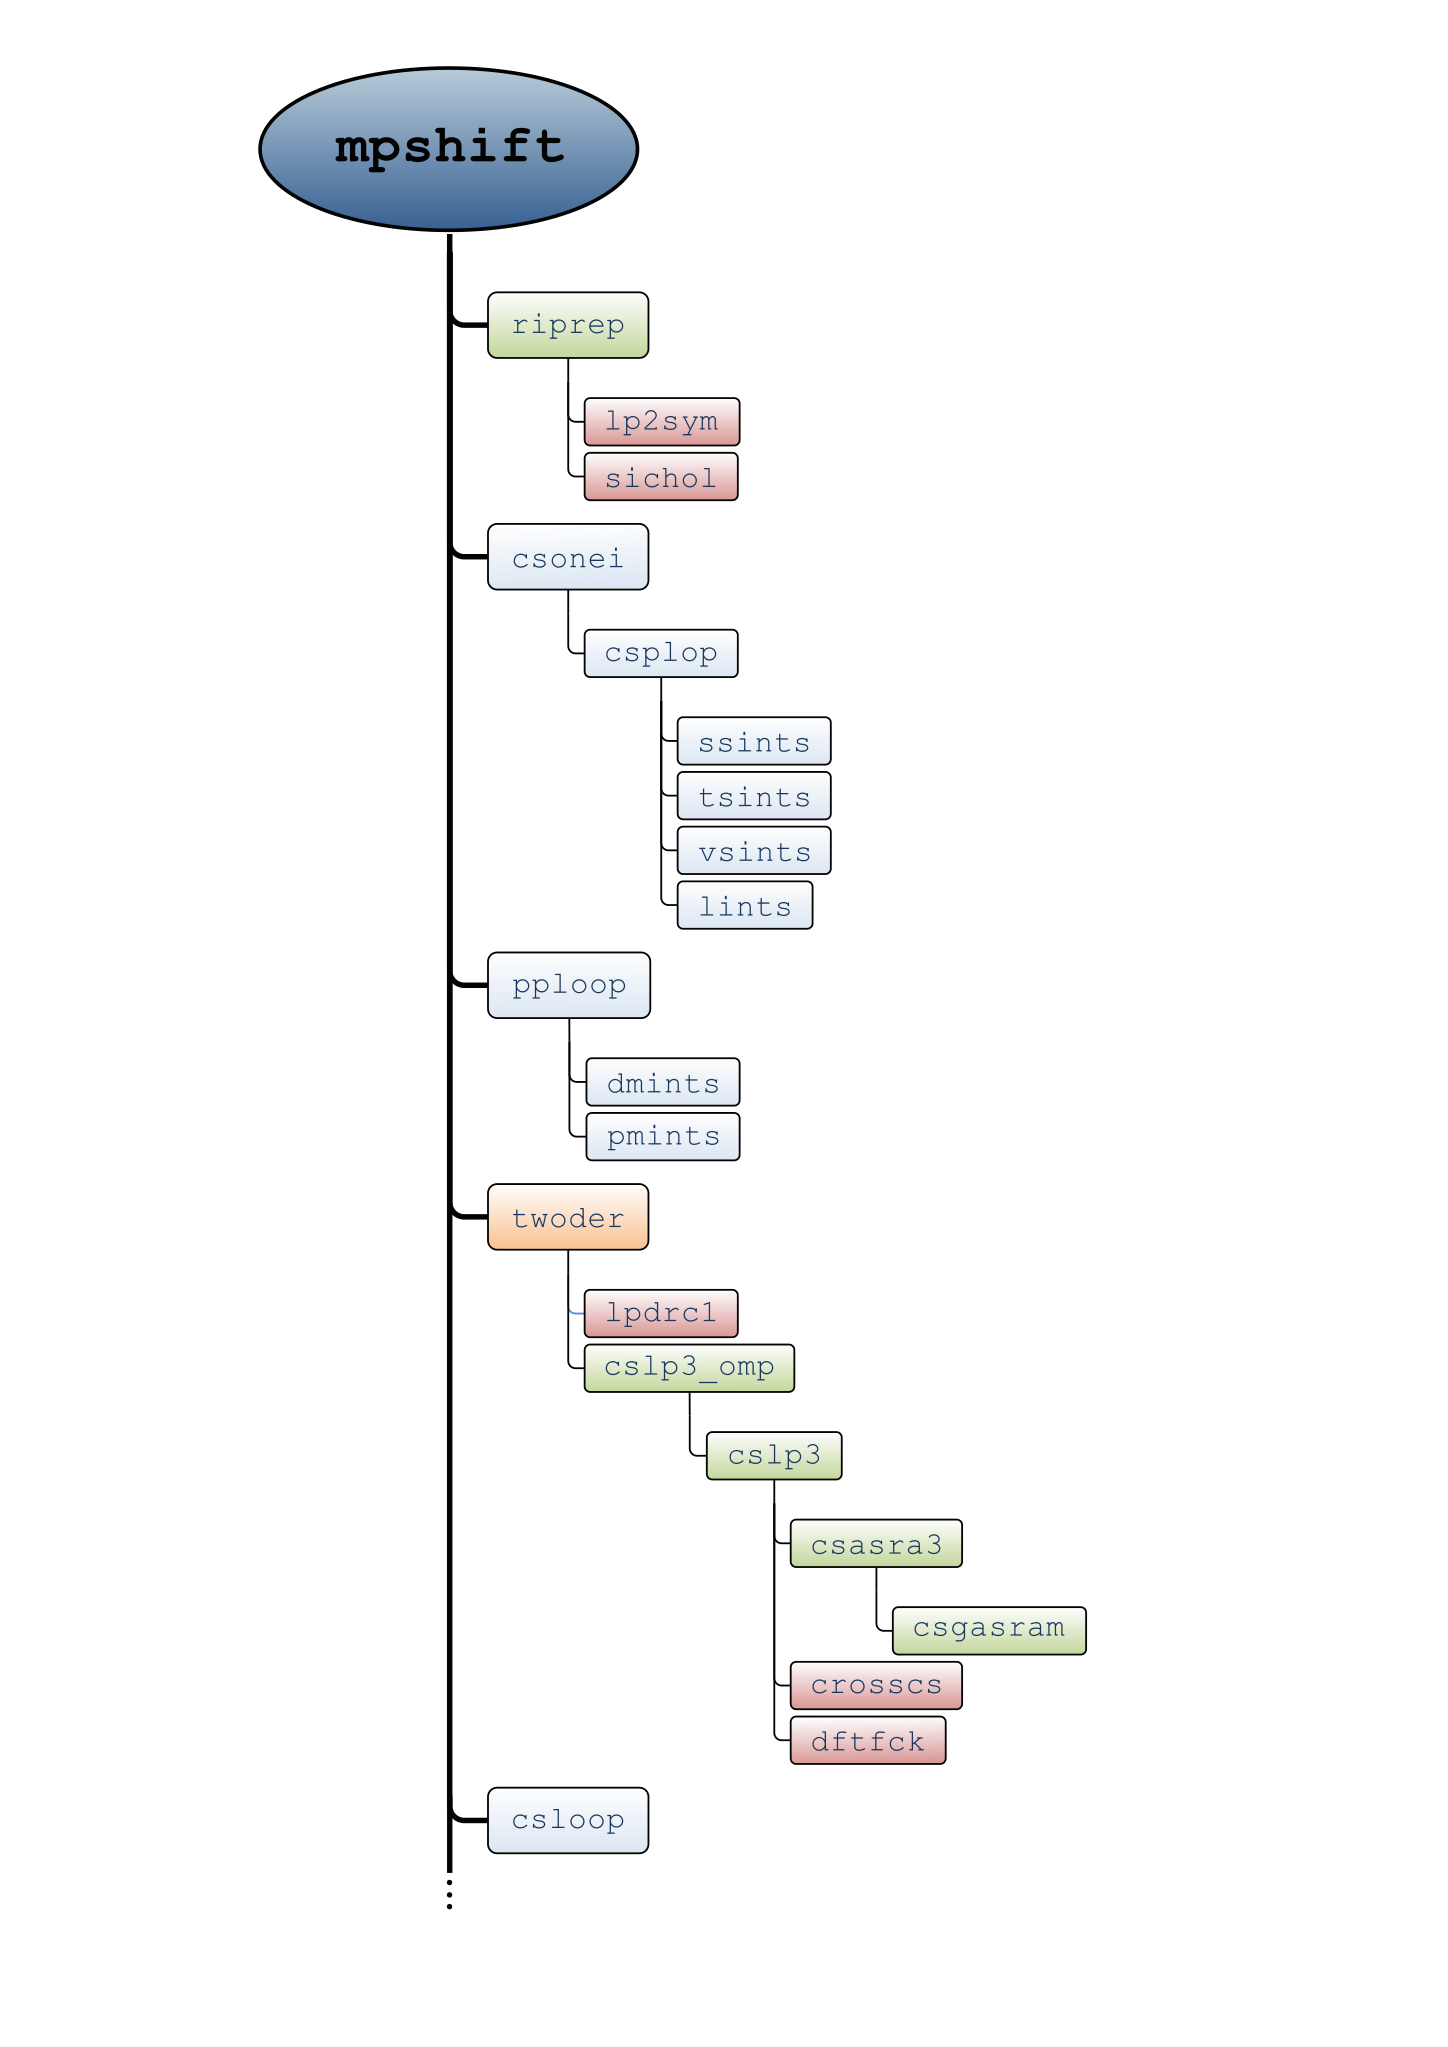
\includegraphics[width=0.6\textwidth]{programmstruktur_ri}
\captionsetup{figurewithin = chapter}
\captionsetup{font=small, labelfont=bf}\caption[RI-J Routinen für chemische Abschirmungskonstanten]{Schematische Darstellung der wichtigsten Routinen für die \ac{ri}-Näherung zur berechnung chemischer Abschirmungskonstanten im Modul \texttt{mpshift}. Alte Routinen sind in blau, neue Routinen in grün, modifizierte Routinen in orange und unverändert übertragene Routinen in rot dargestellt.}
\label{abb:programmstrukur_ri}
\end{figure}

\section{Die MARI-J Methode für chemische Abschirmungskonstanten}\label{marij}
	\subsection{Theorie}
	\subsection{Implementierung}

\section{Seminumerischer Austausch}
	\subsection{Theorie}
	\subsection{Implementierung}
	
\section{Parallelisierung und weitere Optimierungen}\label{paraopt}
Bei bestimmten Verbindungen kann es von Interesse sein, die chemischen Abschirmungskonstanten nur für eine Auswahl an Atomen zu berechnen. Beispielsweise wenn nur eine bestimmte Atomsorte von Interesse ist oder lediglich die chemische Verschiebung in einem bestimmten Bereich untersucht werden soll. In diesen Fällen kann es von Nutzen sein, nur die Beiträge für besagte Atome zu berechnen. Aus diesem Grund wurde das Modul \texttt{mpshift} um die Möglichkeit ergänzt, eine Vorauswahl der zu berechnenden Atome zu treffen. Im Programmcode selbst ist dies auf die einfache Weise realisiert, dass die Ableitungen nach den Komponenten der Kernmomente sowie der gesamte Abschirmungstensor nur für die ausgewählten Atome berechnet wird. Dies kann durch Hinzufügen des Keywords \texttt{\$nucsel} im \texttt{control}-File erreicht werden. Durch die Eingabe von \texttt{\$nucsel "N","Fe"} lassen sich beispielsweise die chemischen Abschirmungskonstanten für alle Sickstoff- und Eisenatome im Molekül berechnen. Mit \texttt{\$nucsel 1,3,5-8} erfolgt die Berechnung für die Atome Nummer 1,3,5-8 im \texttt{coord}-File. Sind in größeren organischen Molekülen, welche von Wasserstoff- und Kohlenstoffatomen dominiert sind, nur die $^1$H bzw. $^13$C Abschirmungskonstanten von Interesse, so bringt dieses vorgehen in der Regel jedoch kaum eine Zeitersparnis und es können direkt alle Atome berechnet werden. Umgekehrt lassen sich auf diese Weise auch Elemente aus der Rechnung herausnehmen, welche ohnehin nicht von Interesse sind, aber gegebenenfalls für ein schlechtes Konvergenzverhalten während der \ac{cphf}-Iterationen sorgen.

\bigskip
Das bisherige, standardmäßige Auswählen des ersten Atoms im \texttt{coord}-File für den Konvergenztest bei den \ac{cphf}-Iterationen lässt sich ebenfalls optimieren. In der Praxis hat sich herausgestellt, dass insbesondere für schwere Elemente mehr Iterationen benötigt werden, bis die Konvergenz erreicht wurde. Dies liegt auch daran, dass die Absolutwerte für die chemischen Abschirmungskonstanten dieser Elemente mit zunehmender Ordnungszahl steigen. Die Konvergenz wurde aber Standardmäßig auf eine Änderung von weniger als \unit[$1\times 10^{-2}$]{ppm} gesetzt, unabhängig von Element. Hierfür wurde ein Faktor eingeführt, welcher die Ordnungszahl des entsprechenden Elements berücksichtigt und die Konvergenz für Elemente mit hoher Ordnungszahl ein wenig lockert. Weiterhin hat sich herausgestellt, dass Atome die weit vom Koordinatenursprung entfernt sind, ebenfalls länger bis zur Konvergenz benötigen. Daher erfolgt die Atomauswahl für den Konvergenztest bei den \ac{cphf}-Iterationen dermaßen, dass zunächst das schwerste Element im Molekül gesucht wird. Sollte es davon mehrere geben, dann wird das Atom ausgewählt, welches am weitesten vom Ursprung entfernt liegt. Dieses Vorgehen hat den Vorteil, dass in der Regel nur in den letzten beiden Iterationen die chemische Verschiebung für alle Atome berechnet werden muss, um zu überprüfen, ob alle Atome bereits konvergiert sind. Da der kritischste Fall zu diesem Zeitpunkt in der Regel bereits zur Konvergenz gebracht werden konnte, ist dies in der Regel gegeben.

\bigskip
Wird die \ac{ri} bzw. \ac{marij}-Methode in einer Hartree-Fock bzw. Hybrid-\ac{dft} Rechnung verwendet, so wird der Austauschbeitrag unabhängig vom Coulombbeitrag berechnet. Für ersteren kann jedoch eine härtere Integralabschätzung angewendet werden, als für den Coulombbeitrag. Aus diesem Grund wurden die Integralabschätzungen aus der Routine \texttt{shloop\_k}, welche ungestörten Austauschmatrixelemente in einer \ac{scf} oder während der \ac{cphf}-Iterationen berechnet, in die Routine \texttt{csloop} übertragen. Auf diese Weise kann die Berechnung kleiner bzw. später verschwindender Matrixelemente vermieden werden. 

\bigskip
Neben einer effizienten Programmierung und dem Einführen von Näherungen wie beispielsweise bei der \ac{ri} bzw. \ac{marij}-Methode, kann die Wartezeit des Nutzers auch durch eine Parallelisierung des Programmcodes reduziert werden. Dies ist insofern von besonderer Bedeutung, dass heutige Computer immer mehr CPUs zur Verfügung haben. Selbst in gewöhnlichen Desktop PCs oder Notebooks finden sich häufig mindestens 4 CPUs. Aus diesem Grund wurden die zeitaufwändigsten Routinen im \texttt{mpshift} Modul mit OpenMP\supercite{dagum1998openmp} in Zusammenarbeit mit Fabian Mack parallelisiert. Im Einzelnen betrifft dies die Routinen \texttt{becke}, \texttt{csloop}, \texttt{cslp3\_omp}, \texttt{csplop},\texttt{shloop\_k} \texttt{p3loop} und \texttt{pploop}. Die Routinen \texttt{csplop}, \texttt{p3loop} und \texttt{pploop} besitzen üblicherweise folgende grundlegende Schleifenstruktur.\\
\\
\texttt{do i=1,N$_{\texttt{Schal}}$}\\ 
\null\quad\texttt{do j=1,N$_{\texttt{Schal}}$}\\ 
\null\quad\quad\texttt{do $\mu$=1,N$_{\texttt{Prim BF}}$}\\ 
\null\quad\quad\quad\texttt{do $\mu$=1,N$_{\texttt{Prim BF}}$}\\
\null\quad\quad\quad\quad \texttt{Auszuführender Programmcode}\\ 
\null\quad\quad\quad\texttt{end do}\\ 
\null\quad\quad\texttt{end do}\\ 
\null\quad\texttt{end do}\\ 
\texttt{end do}\\
\\
Die äußeren beiden Schleifen laufen dabei über alle Schalen N$_{\texttt{Schal}}$ und die beiden inneren Schleifen laufen über die primitiven Basisfunktionen. Für die Routine \texttt{cslp3\_omp} kommt jeweils eine weitere Schleife für die Auxiliarschale und die primitiven Auxiliarbasisfunktionen hinzu. Bei den Vierzentrenroutinen \texttt{csplop} und \texttt{shloop\_k} sind es jeweils zwei weitere Schleifen für die Schalen und die primitiven Basisfunktionen. Bei der Parallelisierung wurde nun in der Regel so vorgegangen, dass die äußersten Schleifen über die Schalen parallelisiert wurden:\\
\\
\texttt{\$OMP PARALLEL}\\
\texttt{\$OMP DO SCHEDULE (DYNAMIC)}\\
\texttt{do i=1,N$_{\texttt{Schal}}$}\\ 
\null\quad\texttt{do j=1,N$_{\texttt{Schal}}$}\\ 
\null\quad\quad\texttt{do $\mu$=1,N$_{\texttt{Prim BF}}$}\\ 
\null\quad\quad\quad\texttt{do $\mu$=1,N$_{\texttt{Prim BF}}$}\\
\null\quad\quad\quad\quad \texttt{Auszuführender Programmcode}\\ 
\null\quad\quad\quad\texttt{end do}\\ 
\null\quad\quad\texttt{end do}\\ 
\null\quad\texttt{end do}\\ 
\texttt{end do}\\
\texttt{\$OMP END DO}\\
\texttt{\$OMP END PARALLEL}\\
\\


\section{Genauigkeit und Effizienz}\label{genauigkeit}

\chapter{Erweiterund der Funktionalität}\label{funktionalität}
Das Modul \texttt{mpshift} umfasste bisher die Möglichkeit zur Berechnung von chemischen Abschirmungskonstanten in Molekülen ohne schwere Elemente (ab etwa $Z$=36) in der Gasphase. Diese Berechnungen konnten auf Hartree-Fock, \ac{dft} (für \ac{lda}- und \ac{gga}-Funktionale) und \ac{mp2} Nievau durchgeführt werden. Des Weiteren konnte die nach den Komponenten des Magnetfeldes abgeleitete Dichtematrix dem externen Programm \ac{gimic} zur Weiterverarbeitung bereit gestellt werden. Die folgenden Kapitel beschreiben die Erweiterung der Funktionalität des Moduls die im Rahmen dieser Arbeit implementiert wurden. Im Einzelnen sind dies die Berücksichtigung relativistischer Effekte auf Nachbaratome in Molekülen mit schweren Elementen durch relativistische \acp{ecp}, die Einbeziehung von Umgebungseffekten sowie die Bereitstellung der magnetischen Response zur Berechnung von \ac{vcd}-Spektren. Weiterhin wurde das Modul um die Möglichkeit ergänzt, \ac{mgga}-Funktionale für die Berechnung der Abschirmungskonstanten auf \ac{dft}-Niveau zu verwenden. Die eigentliche Implementierung dieses letzten Punktes erfolgte jedoch nicht von mir, sondern von Fabian Mack im Rahmen seiner Masterarbeit.\supercite{mack2017} 
\vfill

\section{Berücksichtigung von Umgebungseffekten}
Isotrope chemische Verschiebungen werden üblicherweise in Lösung gemessen. Je nachdem wie stark das zu untersuchende Molekül mit dem Lösungsmittel wechselwirkt, hat das Lösungsmittel einen mehr oder weniger stark ausgeprägten Einfluss auf das gemessene Spektrum. Das \ac{cosmo}\supercite{klamt1993cosmo}, ein Kontinuumsmodell, ist in der Quantenchemie ein bewährtes Verfahren zur Berücksichtigung von Umgebungseffekten. Neben den Einflüssen des Lösungsmittels lassen sich damit für Ionen auch die Ladungen kompensieren ohne die Gegenionen explizit mitrechnen zu müssen. Insbesondere hoch geladene Anionen lassen sich ohne eine solche Ladungskompensation nur schwer oder gar nicht berechnen. 
	\subsection{Theorie}
	\subsection{Implementierung}
	\subsection{Testrechnungen}
	
\section{Skalar-relativistische Effekte durch effektive Kernpotentiale}
	\subsection{Theorie}
	\subsection{Implementierung}
	
\section{Berechnung von Vibrational Circular Dichroism Spektren}
	\subsection{Theorie}
	Die im Experiment gemessenen Intensitäten der \ac{vcd}-Spektroskopie $I_n$ sind proportional zu den in quantenchemischen Rechnungen zugänglichen Rotationsstärken $R_n$. Letztere werden aus dem Skalaprodukt vom \textcolor{myred}{elektrischen/\-elektronischen} und vom magnetischen Übergangsdipolmoment, $\vec{\mu}_n^{\,\text{el}}$ und $\vec{\mu}_n^{\,\text{mag}}$,  erhalten. Somit ergibt sich die \ac{vcd}-Intensität
	\begin{equation}
	  I_n\approx R_n = Im(\vec{\mu}_n^{\,\text{el}}\cdot\vec{\mu}_n^{\text{\,mag}})
	\end{equation}
	für einen Übergang aus dem Schwingungsgrundzustand in den angeregten Schwingungszustand $n$.\supercite{stephens1985theory,stephens1985vibrational} Im Rahmen der harmonishen Näherung sind das \textcolor{myred}{elektrische/\-elektronische} und das magnetische Übergangsdipolmoment gegeben durch \textcolor{myred}{(Zitat?)}
	
	\begin{equation}
	  (\mu_n^{\text{el}})_\beta=\sqrt{\frac{\hbar}{\omega_n}}\sum_{K\alpha}P_{\alpha\beta}^K S_{K\alpha,n}
	\end{equation}
	\begin{equation}
	  (\mu_n^{\text{mag}})_\beta=-\sqrt{2\hbar^3\omega_n}\sum_{K\alpha}M_{\alpha\beta}^KS_{K\alpha,n}.
	\end{equation}
	Hierbei ist $I$ die Zählvariable für die Atomkerne, $\alpha$ und $\beta$ beschreiben kartesische Koordinaten, $\omega_n$ ist die Schwingungsfrequenz der $n$-ten Schwingung und $S_{I\alpha,n}$ ist die Transformationsmatrix von kartesichen zu Normalkoordinaten. Sowohl der sogenannte \ac{apt} (Gleichung (\ref{eq:apt}) als auch der sogenannte \ac{aat} (Gleichung (\ref{eq:aat})) lassen sich in einen elektronischen und einen Kernbeitrag aufteilen
	\begin{equation}\label{eq:apt}
	  P^K_{\alpha\beta}=E^K_{\alpha\beta}+N^K_{\alpha\beta}
	\end{equation}
	\begin{equation}\label{eq:aat}
   	  M^K_{\alpha\beta}=I^K_{\alpha\beta}+J^K_{\alpha\beta}.
	\end{equation}
	Die Berechnung der Kernbeiträge 
	\begin{equation}
	  N^K_{\alpha\beta}=eZ_K\delta_{\alpha\beta}
	\end{equation}
	\begin{equation}
	  J^K_{\alpha\beta}=\iu\frac{eZ_K}{4\hbar c}\sum_K^{N_K}\varepsilon_{\alpha\beta\gamma}R^0_{K\gamma}
	\end{equation}
	ist trivial. $e$ ist die Elementarladung, $Z_K$ ist die Ladung des Kerns $K$ und $\delta_{\alpha\beta}$ ist das Kroneckerdelta. $c$ ist die Lichtgeschwindigkeit und $\varepsilon_{\alpha\beta\gamma}$ ist der Levi-Civita-Permutationstensor. Die Position des Kerns $K$ ist durch $R^0_{K\gamma}$ gegeben, wobei $\gamma$ für eine der drei kartesischen Raumkoordinaten steht und die hochgestellte $0$ symbolisiert die Auswertung in der Gleichgewichtsgeometrie.   
	
    Zur Berechnung der elektronischen Beiträge 
    \begin{equation}
      E^K_{\alpha\beta}=\left(\sum_{i=1}^{N_{\text{occ}}}\frac{\partial \langle\phi_i\vert r_\beta\vert\phi_i\rangle}{\partial R_{K\alpha}}\right)_{\vec{R}^0}
    \end{equation}
    \begin{equation}\label{eq:vcdaatel}
      I^K_{\alpha\beta}=\sum_{i=1}^{N_{\text{occ}}}=\left\langle\left.\left(\frac{\partial \phi_i}{\partial R_{K\alpha}}\right)_{\vec{R}^0}\right|\left(\frac{\partial \phi_i}{\partial B_\beta}\right)_{\vec{B}=0}\right\rangle
    \end{equation}
    
    ist ein deutlich größerer Aufwand erforderlich. Die $\phi_i$ sind die besetzten \acp{mo}. Wie bereits in Kapitel \ref{theo:nmr} beschrieben, lasst sich die \ac{mo}-Ableitung nach einer Komponente des externen magnetischen Feldes im Rahmen des \ac{cphf}-Formalismus als 
    \begin{equation}\label{eq:vcdcphf}
    \left(\frac{\partial \phi_i}{\partial B_\beta}\right)_{\vec{B}=0}=\phi_i^{B_\beta}=\sum_{\mu=1}^{N_{\text{BF}}}\left[c_{\mu i}\chi_\mu^{B_\beta}+\sum_{p=1}^{N_{\text{MO}}}c_{\mu p}U_{ip}^{B_\beta}\chi_\mu\right]
	\end{equation}
	ausdrücken. Die Koeffizientenmatrix $U_{ip}^{B_\beta}$ beschreibt die Änderung der Molekülorbitale durch die Störung des äußeren Magnetischen Feldes $\vec{B}$. Sie wird durch Lösen der entsprechenden \ac{cphf}-Gleichungen erhalten, ganz analog zur Vorgehensweise bei der Berechnung von \ac{nmr}-Abschirmkonstanten. Durch die Kombination der Gleichungen (\ref{eq:vcdaatel}) und  (\ref{eq:vcdcphf}) wird der zu implementierende Ausdruck für den elektronischen Anteil des \ac{aat} erhalten
	\begin{equation}\label{eq:vcdaatelfinal}
	\begin{aligned}
	I^K_{\alpha\beta}=&\sum_{i=1}^{N_{\text{occ}}}\sum_{\mu,\nu=1}^{N_{\text{BF}}}\left[c_{\mu i}c_{\nu i}\left\langle\chi_\mu^{R_{K\alpha}}\vert\chi_\nu^{B_\beta}\right\rangle+\sum_{p=1}^{N_{\text{MO}}}c_{\mu i}c_{\nu p}U_{ip}^{B_\beta}\left\langle\chi_\mu^{R_{K\alpha}}\vert\chi_\nu\right\rangle\right.\\
	&\left.+\sum_{p=1}^{N_{\text{MO}}}c_{\mu i}c_{\nu p}U_{ip}^{R_{K\alpha}}\left\langle\chi_\mu\vert\chi_\nu^{B_{\beta}}\right\rangle+\sum_{p,q=1}^{N_{\text{MO}}}c_{\mu p}c_{\nu q}U_{ip}^{R_{K\alpha}}U_{iq}^{B_\beta}\left\langle\chi_\mu\vert\chi_\nu\right\rangle\right].
	\end{aligned}
	\end{equation}
	Durch die Koeffizientenmatrix $U_{ip}^{R_{K\alpha}}$ wird die Response der Wellenfunktion auf die Verrückung des Kerns $K$ beschrieben. Analog zu $U_{ip}^{B_\beta}$ werden auch sie durch Lösen der entsprechenden \ac{cphf}-Gleichungen erhalten. Gebraucht werden sie ebenfalls zur Berechnung von Kraftkonstanten, wie sie im \textsf{Turbomole} Modul \texttt{aoforce}\supercite{deglmann2002efficient} berechnet werden.
	\subsection{Implementierung}
	Die in Gleichung (\ref{eq:vcdaatelfinal}) auftretenden Integrale, welche die Ableitung nach dem externen magnetischen Feld enthalten, lassen sich für die $x$-Komponente des $B$-Feldes wie folgt umschreiben
	
	\begin{equation}
	\begin{aligned}
	  \left\langle\chi_\mu\vert\chi_\nu^{B_x}\right\rangle&=\left.\left\langle\chi_\mu\left|\frac{\partial}{\partial B_x}\right.\chi_\nu\right\rangle\right|_{\vec{B}=0}=\left\langle\chi_\mu^{\vec{B}=0}\left|\frac{-\iu}{2c}\left(R_{\nu y}z-R_{\nu z}y\right)\right|\chi_\nu^{\vec{B}=0}\right\rangle\\
	  &=\frac{\iu}{2c}\left(R_{\nu z}\left\langle\chi_\mu^{\vec{B}=0}\left|y\right|\chi_\nu^{\vec{B}=0}\right\rangle-R_{\nu y}\left\langle\chi_\mu^{\vec{B}=0}\left|z\right|\chi_\nu^{\vec{B}=0}\right\rangle\right).
	\end{aligned}
	\end{equation}
	
	Analog ergeben sich die Ableitungen nach der $y$- 
	
		\begin{equation}
	  \left\langle\chi_\mu\vert\chi_\nu^{B_y}\right\rangle=\frac{\iu}{2c}\left(R_{\nu x}\left\langle\chi_\mu^{\vec{B}=0}\left|z\right|\chi_\nu^{\vec{B}=0}\right\rangle-R_{\nu z}\left\langle\chi_\mu^{\vec{B}=0}\left|x\right|\chi_\nu^{\vec{B}=0}\right\rangle\right)
	\end{equation}
	
	und $z$-Komponente
	
		\begin{equation}
	  \left\langle\chi_\mu\vert\chi_\nu^{B_z}\right\rangle=\frac{\iu}{2c}\left(R_{\nu y}\left\langle\chi_\mu^{\vec{B}=0}\left|x\right|\chi_\nu^{\vec{B}=0}\right\rangle-R_{\nu x}\left\langle\chi_\mu^{\vec{B}=0}\left|y\right|\chi_\nu^{\vec{B}=0}\right\rangle\right).
	\end{equation}

\section{meta-GGA Funktionale}
	\subsection{Theorie}
	\subsection{Implementierung}
	
	



\chapter{Anwendungen}\label{anwendungen}
\section{Anwendungen in der anorganischen Chemie}
\subsection{[SIMesPGa\textit{t}Bu$_2$]$_2$, [SIMesP(Ga\textit{t}Bu$_2$)$_2$Cl] und [K(SIMesP)$_3$Al\textit{t}Bu]}
\subsection{[Hg$_8$Te$_8$(Te$_2$)$_4$]$^{8-}$: Ein anorganisches Porphyrin?}
\begin{figure}[ht!]
	\centering
	\includegraphics[width=0.6\textwidth]{hgte_1bohr}
	\captionsetup{figurewithin = chapter}
	\captionsetup{font=small, labelfont=bf}\caption[]{.}
\label{abb:hgtelic}
\end{figure}

\begin{figure}[ht!]
	\centering
	\includegraphics[width=0.6\textwidth]{porph_1bohr}
	\captionsetup{figurewithin = chapter}
	\captionsetup{font=small, labelfont=bf}\caption[]{.}
\label{abb:porphlic}
\end{figure}

\begin{figure}[ht!]
	\centering
	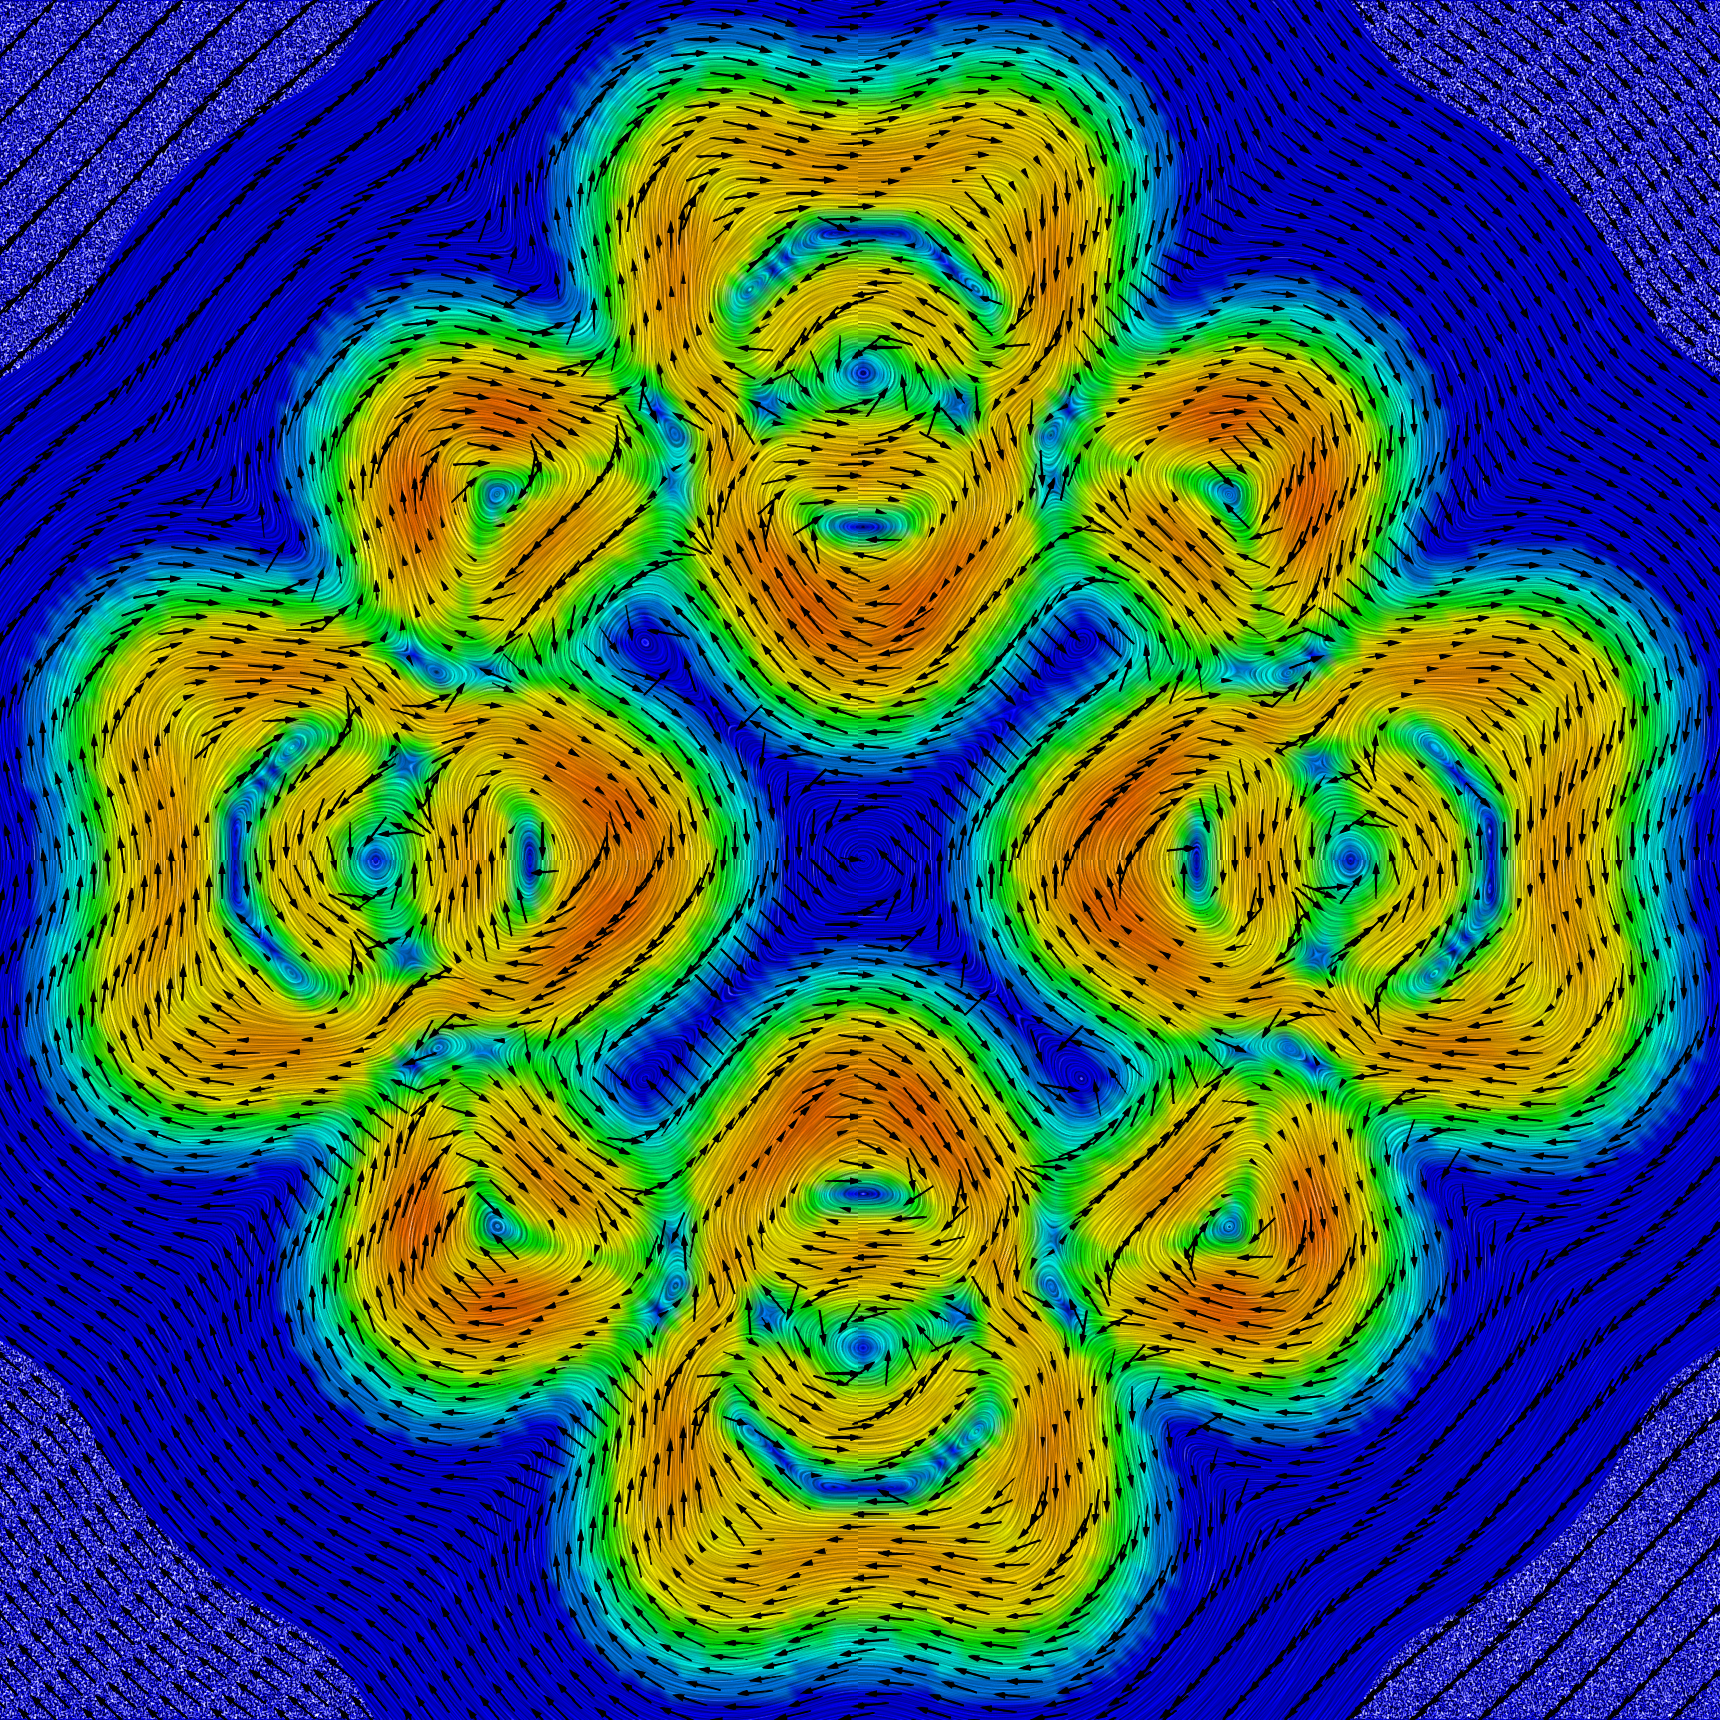
\includegraphics[width=0.6\textwidth]{b8s16_1bohr}
	\captionsetup{figurewithin = chapter}
	\captionsetup{font=small, labelfont=bf}\caption[]{.}
\label{abb:b8s16hlic}
\end{figure}

\begin{figure}[ht!]
	\centering
	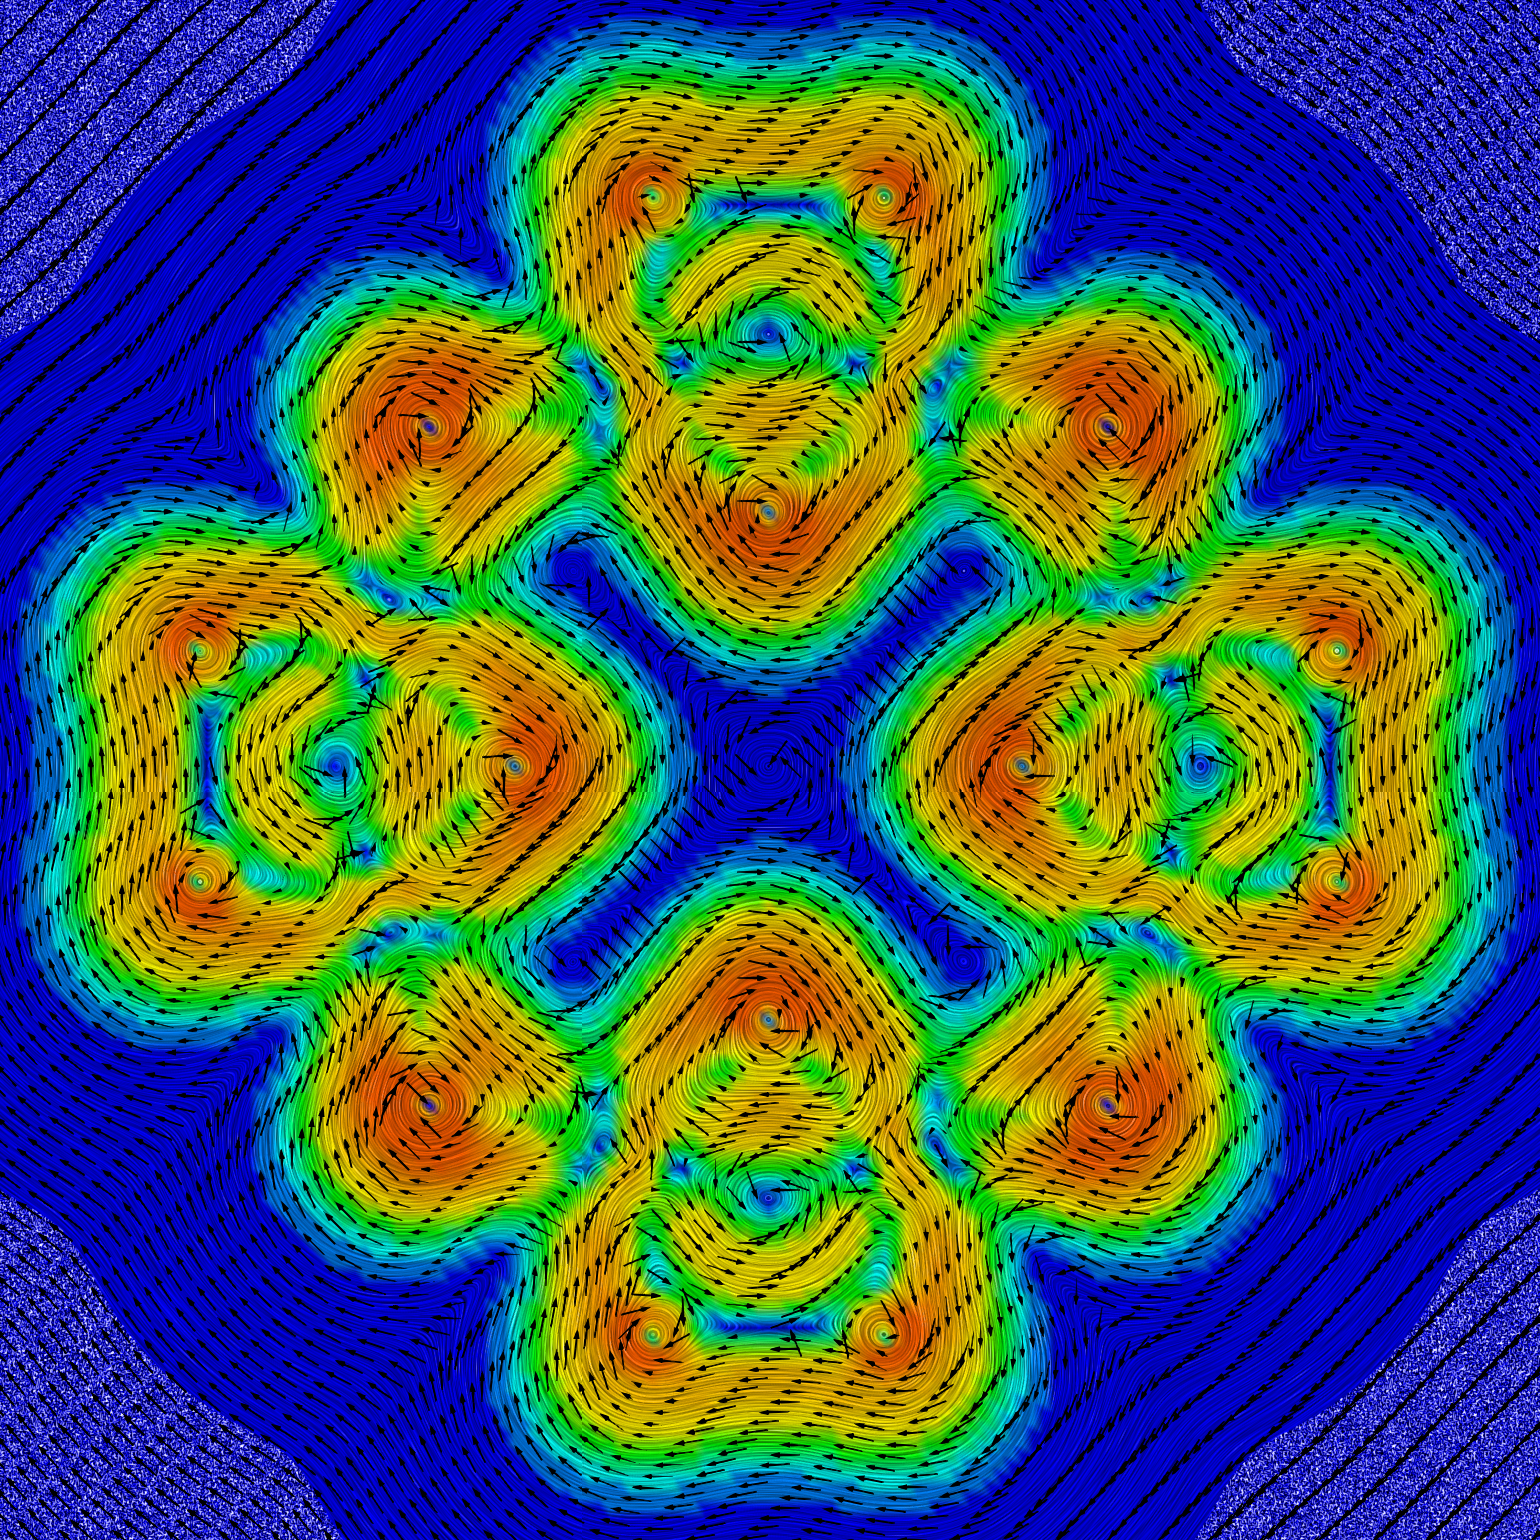
\includegraphics[width=0.6\textwidth]{b8se16_1bohr}
	\captionsetup{figurewithin = chapter}
	\captionsetup{font=small, labelfont=bf}\caption[]{.}
\label{abb:b8se16hlic}
\end{figure}
\subsection{[Co\@Sn$_6$Sb$_6$]$^{3-}$}
\section{Ringströme in großen ringförmigen Kohlenstoffnanoröhren}

\chapter{Zusammenfassung}\label{zusammenfassung}
\begin{figure}[ht!]
	\centering
	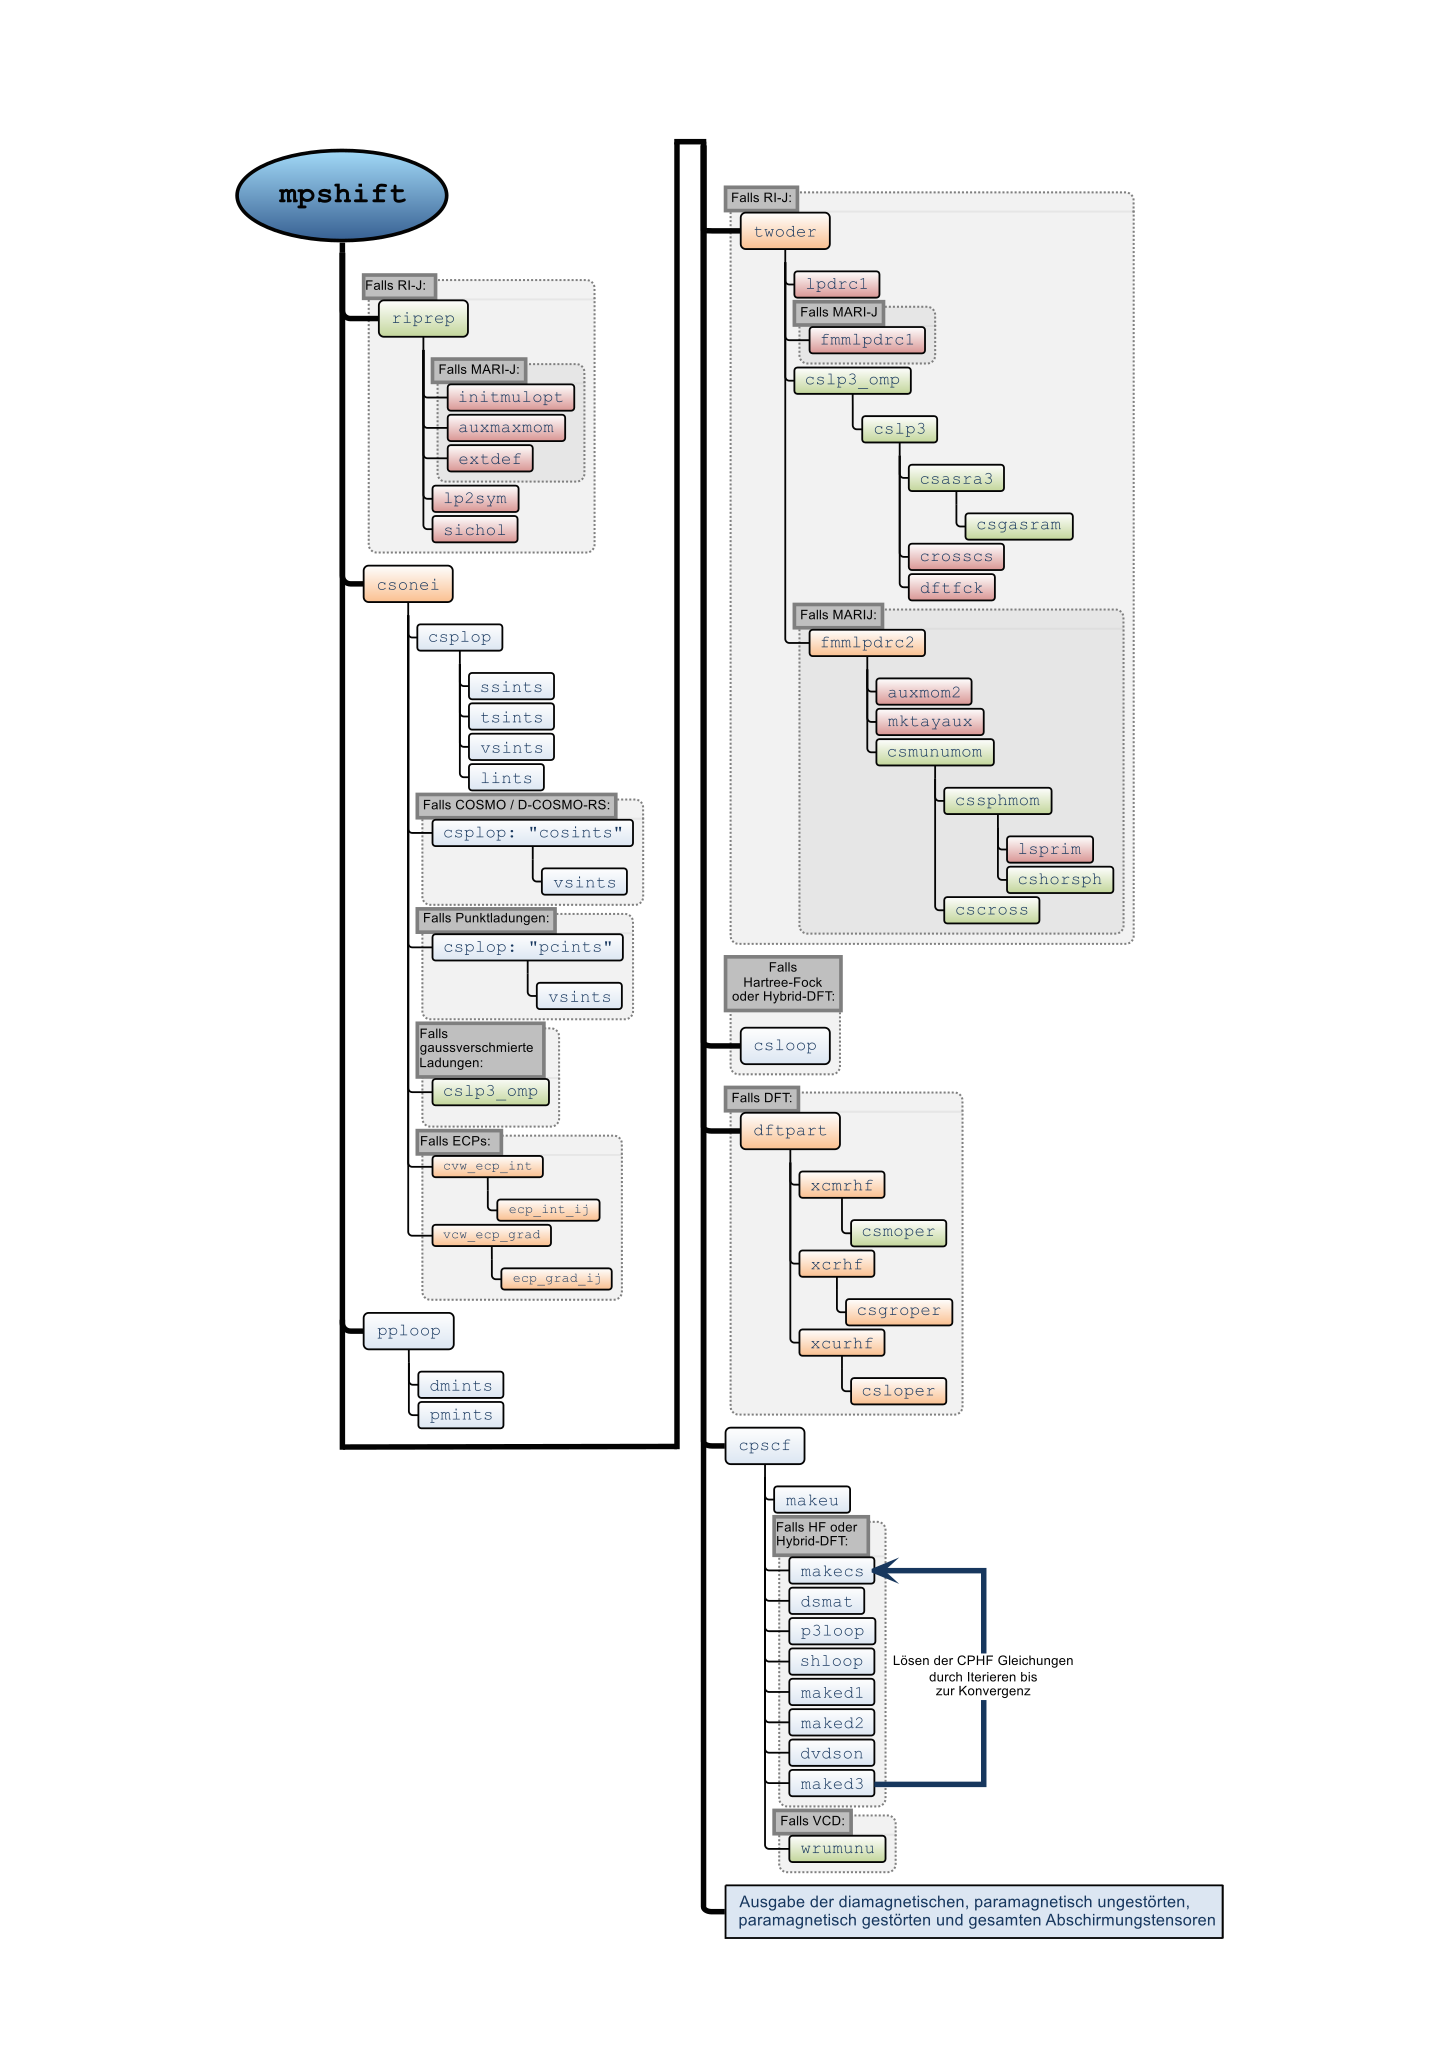
\includegraphics[width=1.0\textwidth]{mpshift_all}
	\captionsetup{figurewithin = chapter}
	\captionsetup{font=small, labelfont=bf}\caption[Neue schematische Programmstruktur des Moduls \texttt{mpshift}]{Schematische Programmstruktur des Moduls \texttt{mpshift} mit den wichtigsten Änderungen und Erweiterungen die im Rahmen der vorliegenden Arbeit durchgeführt wurden. Alte Routinen sind in blau, neue Routinen in grün, modifizierte Routinen in orange und unverändert aus anderen Modulen übertragene Routinen in rot dargestellt.}
\label{abb:neue_programmstruktur}
\end{figure}


% Schlussteil - Römische Seitennummerierung
\backmatter
%\pagenumbering{Roman}
%\setcounter{page}{9}

\begingroup
	\renewcommand*{\addvspace}[1]{}
	\phantomsection
	\listoffigures
\endgroup

\begingroup
	\renewcommand*{\addvspace}[1]{}
	\phantomsection
	\listoftables
\endgroup
\newpage
\phantomsection \addcontentsline{toc}{chapter}{Abkürzungsverzeichnis}
\renewcommand\refname{Abkürzungsverzeichnis} \chapter*{Abkürzungsverzeichnis}
\begin{acronym}[SEPSEP] % längste Abkürzung steht in eckigen Klammern
    \setlength{\itemsep}{0.2cm} % geringerer Zeilenabstand
    
    \acro{aat}[AAT]{\textit{atomic axial tensor}}
    
    \acro{apt}[APT]{\textit{atomic polar tensor}}
    
    \acro{ao}[AO]{Atomorbital}
	\acro{caac}[CAAC]{cyclisches Alkylaminocarben}   
		\acrodefplural{caac}[CAACs]{cyclischen Alkylaminocarbenen}
	\acro{carac}[CArAC]{cyclisches Arylaminocarben}
		\acrodefplural{carac}[CArACs]{cyclische Arylaminocarbene}
		
    \acro{cc}[CC]{Coupled Cluster}		
		
 	\acro{cosmo}[COSMO]{\textit{Conductor-like Screening Model}}
 	
	\acro{cphf}[CPHF]{\textit{coupled perturbed Hartree-Fock}}
	
	\acro{csm}[CSM]{Continuum Solvatiol Model}
 	
    \acro{dft}[DFT]{Dichtefunktionaltheorie}
    
    \acro{diis}[DIIS]{\textit{Direct Inversion of the Iterative Subspace}}
    
    \acro{dipp}[dipp]{2,6-Diisopropylphenyl}
    
    \acro{ecp}[ECP]{\textit{Effective-Core-Potential}}
    
    \acro{esp}[ESP]{elektrostatisches Potential}
	    \acrodefplural{esp}[ESP]{elektrostatischen Potentials}
	
	\acro{giao}[GIAO]{\textit{Gauge Including Atomic Orbital}}   
	
	\acro{gimic}[GIMIC]{\textit{Gauge Including Magnetically Induced Currents}} 

	\acro{gga}[GGA]{\textit{Generalized-Gradient-Approximation}}   
		\acrodefplural{gga}[GGA]{\textit{Generalized-Gradient-Approximation}}
		
	\acro{lcao}[LCAO]{\textit{Linear Combination of Atomic Orbitals}}
	\acro{lda}[LDA]{\textit{Local-Density-Approximation}}
     
    \acro{marij}[MARI-J]{\textit{Multipole Accelerated Resolution of the Identity for $J$}} 	
 	
	\acro{mgga}[MGGA]{\textit{Meta}-GGA}   
		\acrodefplural{mgga}[MGGA]{\textit{Meta}-GGA}	
	\acro{mo}[MO]{Molekülorbital}   
		\acrodefplural{mo}[MOs]{Molekülorbitale}
		
	\acro{md}[MD]{Molekular-Dynamik}
	
	\acro{mp2}[MP2]{M\o ller-Plesset Störungstheorie zweiter Ordnung}
		
    \acro{nao}[NAO]{\textit{Natural-Atomic-Orbital}}

    \acro{nbo}[NBO]{\textit{Natural-Bond-Orbital}}
    
    \acro{nmr}[NMR]{\textit{Nuclear Magnetic Resonace}}
        
    \acro{npa}[NPA]{\textit{Natural-Population-Analysis}}
    
    \acro{oswo}[OWSO]{\textit{Occupancy-Weighted-Symmetric-Orthogonalization}}
    
    \acro{ri}[RI]{\textit{Resolution of the Identity}}
    
	\acro{scf}[SCF]{\textit{Self Consistent Field}}   

	\acro{tep}[TEP]{Tolmans elektronischer Parameter}   
		\acrodefplural{tep}[TEPs]{Tolmans elektronische Parameter}
		
	\acro{vcd}[VCD]{\textit{Vibrational Circular Dichroism}}

    

        
    \acro{vmd}[VMD]{Visual Molecular Dynamics}
\end{acronym}

\printbibliography[title=Literaturverzeichnis]

\chapter*{Veröffentlichungen}
\markboth{Veröffentlichungen}{} %chapterheader trotz * anzeigen lassen
\begin{enumerate}
%\item \textit{•}\\ \textit{•} \textbf{•}

\item \textit{Size Matters: From Two Dimensional Au(I)-Tl(I) Metallopolymers to Molecular Complexes}\\
T. Seifert, N. Knoefel, T. Feuerstein, K. Reiter, S. Lebedkin, M. Gamer, A. Boukis, F. Weigend, M. Kappes, P. Roesky, in Vorbereitung (2018).

\item \textit{[Co@Sn$_6$Sb$_6$]$^{3-}$: Structure and $^{119}$Sn NMR Spectrum of an Off-Center Endohedral 12-Vertex Cluster}\\
R. J. Wilson, F. Hastreiter, K. Reiter, P. Büschelberger, R. Wolf, R. Gschwind, F. Weigend, S. Dehnen, eingereicht (2018).

\item \textit{[Hg$_4$Te$_8$(Te$_2$)$_4$]$^{8-}$: A Heavy Metal Porphyrinoid Embedded in a Lamellar Structure}\\
C. Donsbach, K. Reiter, D. Sundholm, F. Weigend, S. Dehnen, \textit{Angew. Chem. Int. Ed.} \textbf{57}, 8770, (2018).

\item \textit{Multicomponent Reactions Provide Key Molecules for Secret Communication}\\ 
A. Boukis, K. Reiter, M. Frölich, D. Hofheinz, M. Meier, \textit{Nat. Commun.} \textbf{9}, 1439 (2018).

\item \textit{(Ge$_2$P$_2$)$^{2-}$: A Binary Analogue of P$_4$ as a Precursor to the Ternary Cluster Anion [Cd$_3$(Ge$_3$P)$_3$]$^{3-}$}\\
S. Mitzinger, J. Bandemehr, K. Reiter, J. McIndoe, X. Xie, F. Weigend, J. Corrigan, S. Dehnen, \textit{Chem. Commun.} \textbf{54}, 1421 (2018).

\item \textit{Calculation of Magnetic Shielding Constants with meta-GGA Functionals Employing the Multipole-Accelerated Resolution of the Identity: Implementation and Assessment of Accuracy and Efficiency}\\ 
K. Reiter, F. Mack, F. Weigend, \textit{J. Chem. Theory Comput.} \textbf{14}, 191 (2018).

\item \textit{An NHC-Phosphinidenyl as a Synthon for New Group 13/15 Compounds}\\
O. Lemp, M. Balmer, K. Reiter, F. Weigend, C. von Hänisch, \textit{Chem. Commun.} \textbf{53}, 7620 (2017).

\item \textit{Vibrational Circular Dichroism Spectra for Large Molecules and Molecules with Heavy Elements}\\
K. Reiter, M. Kühn, F. Weigend, \textit{J. Chem. Phys.} \textbf{146}, 054102 (2017).

\item \textit{A Dinuclear Gold(I) Bis(Carbene) Complex Based on a Ditopic Cyclic (Aryl)\\(Amino)Carbene Framework}\\
E. Deck, K. Reiter, W. Klopper, F. Breher, \textit{Z. Anorg. Allg. Chem.} \textbf{642}, 1320 (2016).

\item \textit{A Boron-Fluorinated Tris(pyrazolyl)borate Ligand ($^FTp^*$) and Its Mono- and Dinuclear Copper Complexes [Cu($^FTp^*$)$_2$] and [Cu$_2$($^FTp^*$)$_2$]: Synthesis, Structures, and DFT Calculations}\\
T. Augenstein, F. Dorner, K. Reiter, H. Wagner, D. Garnier, W. Klopper, F. Breher, \textit{Chem. Eur. J.} \textbf{22}, 7935 (2016).

\item \textit{[(Pb$_6$I$_8$)\{Mn(CO)$_5$\}$_6$]$^{2-}$: An Octahedral (M$_6$X$_8$)-like Cluster with Inverted Bonding}\\
S. Wolf, K. Reiter, F. Weigend, W. Klopper, C. Feldmann, \textit{Inorg. Chem.} \textbf{54}, 3989 (2015).
\end{enumerate}

\chapter*{Lebenslauf}
\markboth{Lebenslaug}{} %chapterheader trotz * anzeigen lassen
\renewcommand{\arraystretch}{1.7}
\begin{singlespace}
\begin{tabular}{lp{7.6cm}}
Name: & Kevin Reiter \\ 

Geburtsdatum: & 29. November 1989 \\ 

Geburtsort: & Neuenbürg \\ 

\quad & \quad \\

1996 - 2000 & Wilhelm-Ganzhorn-Grundschule Straubenhardt \\ 

2000 - 2009 & Gymnasium Neuenbürg \\ 

Juni 2009 & allgemeine Hochschulreife \\ 

2010 - 2013 & Bachelor Studium Chemie am Karlsruher Institut für Technologie  \\ 
Juni 2013 - August 2013  & Bachelorarbeit am Institut für Physikalische Chemie, Abteilung für Theoretische Chemie am Karlsruher Institut für Technologie unter Anleitung von Prof. Dr. Willem Klopper \\

Oktober 2013 & Abschlus als Bachelor of Science \\ 
 
2013 - 2015 & Master Studium Chemie am Karlsruher Institut für Technologie \\ 

März 2015 - September 2015  & Masterarbeit am Institut für Physikalische Chemie, Abteilung für Theoretische Chemie am Karlsruher Institut für Technologie unter Anleitung von Prof. Dr. Willem Klopper \\

September 2015 & Abschlus als Master of Science \\ 

2015 & Beginn der Promotion am Institut für Physikalische Chemie, Abteilung für Theoretische Chemie am Karlsruher Institut für Technologie unter Anleitung von PD Dr. Florian Weigend \\ 

November 2017 - Dezember 2017 & 6-wöchiger Forschungsaufenthalt an der Universität Helsinki bei Prof. Dr. Dage Sundholm \\ 
\end{tabular}  
\end{singlespace}
\enlargethispage{13.5pt}
\vfill
\newpage
\thispagestyle{empty}
\quad
\chapter*{Danksagung}
\markboth{Danksagung}{} %chapterheader trotz * anzeigen lassen
%\thispagestyle{empty}
Zu Beginn möchte ich mich bei meinen Mathematik-, Physik- und Chemielehrern Michael Frey, Matthias Sickmüller und Michael Burkard bedanken, die zur rechten Zeit mein Interesse an den Naturwissenschaften gefördert und gefordert haben. Ich danke ihnen für ihren lehrreichen und vorbildlichen Unterricht, auch wenn das einige meiner ehemaligen Mitschüler sicher anders sehen würden.

\bigskip
Mein größter Dank gilt PD Dr. Florian Weigend für eine Betreuung, wie sie nicht hätte besser sein können. Insbesondere für seine unermüdliche Unterstützung bei noch so kleinen Fragen und Problemen, all die anregenden Gespräche und auch für die Freiheiten, die er mir gelassen hat. Die Momente abseits der Wissenschaft und die Vermittlung der wirklich wichtigen Kompetenzen -- am Kickertisch -- werden mir immer in bester Erinnerung bleiben. Eine wahrhaft vorbildliche Zusammenarbeit zwischen einem Schwaben und einem Badener.

\bigskip
Prof. Dr. Burkhard Luy danke ich vielmals für die Übernahme des Koreferats.

\bigskip
Bei Prof. Dr. Willem Klopper möchte ich mich für die Finanzierung zu Beginn meiner Promotion bedanken. Weiterhin danke ich ihm für die Nutzung der am Lehrstuhl für Theoretische Chemie zur Verfügung stehenden Ressourcen. Nicht zuletzt bin ich dankbar für die Zeit und die Betreuung während meiner Bachelor-, Vertiefungs- und Masterarbeit, was mein Interesse an der Theoretischen Chemie vertieft und letztlich zu dieser Arbeit geführt hat.

\bigskip
Besonderer Dank gilt meinem langjährigen Bürokollegen Christof Holzer mit dem ich nun seit einiger Zeit das \glqq vormals Badisch Birro\grqq{} besetze. Es war und ist eine tolle Zeit zusammen mit ihm, sowohl im Büro als auch auf diversen Konferenzen oder Wanderungen, egal ob in Mariapfarr, Bochum, München oder Helsinki.

\bigskip
Dr. Markus Armbruster danke ich für die gemeinsame Zeit im damals noch \glqq Badische Birro\grqq{} und seine Hilfsbereitschaft meine Fragen zu beantworten. 

Dr. Michael Kühn und Fabian Mack danke ich für die Zusammenarbeit am VCD- und Meta-GGA-Projekt.  

\bigskip
Prof. Dr. Dage Sundholm danke ich für seine Gastfreundschaft während meiner beiden Aufenthalte in Helsinki sowie für die Betreuung während meines Forschungsaufenthalts. In diesem Zusammenhang sollen auch Maria Dimitrova und Dr. Lukas Wirz nicht unerwähnt bleiben.
%\newpage
%\thispagestyle{empty}

Dr. Michael Harding, Frank Imhoff und Sebastian Kleinhans gilt mein Dank für alle technischen Angelegenheiten sowie für die Lösung von Problemen bei Soft- und Hardwarefragen. 

Weiter danke ich allen zeitweiligen oder noch aktiven Mitgliedern in der Abteilung für Theoretische Chemie, die ich während meiner Zeit dort -- seit meiner Bachelorarbeit -- kennenlernen durfte, für die tolle Zeit und auch für die nicht immer fachlichen Gespräche. Dazu gehören insbesondere Dr. Angela Bihlmeier, Dr. Katharina Krause, Dr. Jiří Chmela, Dr. Johannes Heuser, Dr. Nils  Middendorf, Nils Schieschke, Dr. Patrik Pollak, Dr. Peter Limacher und Yannick Franzke.

Unserer Sekretärin Manuela Kühn danke ich für ihre Hilfe bei allen organisatorischen und bürokratischen Angelegenheiten, die sie immer gerne übernommen hat, obwohl ich eigentlich am INT im Norden angestellt bin.

\bigskip
Für die kritische und äußerst aufmerksame Durchsicht der Arbeit bedanke ich mich bei Fabian Mack und Yannick Franzke.

\bigskip
Außerdem gilt mein Dank dem SFB 1176 \glqq Strukturierung weicher Materie\grqq{} der Deutschen Forschungsgemeinschaft (DFG) für die finanzielle Unterstützung.

\bigskip
Meinen Eltern und meiner Familie danke ich für das grenzenlose Vertrauen und die Unterstützung meiner Vorhaben seit jeher. 

\bigskip
Meiner Freundin Martina Hadamjetz danke ich für ihre bedingungslose Liebe und die wundervolle gemeinsame Zeit. 
%Schliesslich danke ich s`Madame fuer ihre Liebe :)

\newpage
\thispagestyle{empty}
\quad

%Abkürzungen ausgeben
\deftranslation[to=German]{Acronyms}{Abkürzungsverzeichnis}
\printglossary[type=\acronymtype,style=long]
% ---------------------------------------------------------------
% Anhang
\appendix
%\includepdf[pages=-,fitpaper=true,addtotoc={1,section,0,Diagramm: Vergabe,fig:Vergabedia}]{Pfad-zu-einem-pdf-dokument.pdf}
\end{document}